% !TEX TS-program = arara
% arara: xelatex: { synctex: on, options: [--halt-on-error] } 
% arara: biber
% arara: makeglossaries
% arara: makeindex
% arara: xelatex: { synctex: on, options: [-halt-on-error] } 
% arara: xelatex: { synctex: on, options: [-halt-on-error] } 
% arara: clean: { files: [arithmetic-notes.aux,arithmetic-notes.bbl] }
% arara: clean: { files: [arithmetic-notes.bcf,arithmetic-notes.blg] }
% arara: clean: { files: [arithmetic-notes.glg,arithmetic-notes.glo] }
% arara: clean: { files: [arithmetic-notes.gls,arithmetic-notes.gls] }
% arara: clean: { files: [arithmetic-notes.idx,arithmetic-notes.ilg] }
% arara: clean: { files: [arithmetic-notes.ind,arithmetic-notes.loe] }
% arara: clean: { files: [arithmetic-notes.lof,arithmetic-notes.log] }
% arara: clean: { files: [arithmetic-notes.log,arithmetic-notes.lol] }
% arara: clean: { files: [arithmetic-notes.out] }
% arara: clean: { files: [arithmetic-notes.run.xml] }
% arara: clean: { files: [arithmetic-notes.toc,arithmetic-notes.xdy] }
% arara: clean: { files: [arithmetic-notes.synctex.gz] }
%-------------------------------------------------------------------------------
\documentclass[10pt,openany]{book}
%-------------------------------------------------------------------------------
\errorcontextlines 10000
%-------------------------------------------------------------------------------
%input path
%-------------------------------------------------------------------------------
\makeatletter
\def\input@path{{../figs/}{../tex/}{../rawtex/}{../}}
\makeatother
%-------------------------------------------------------------------------------
% TODO: try these
% \usepackage{amsmath,amsfonts,amssymb,mathrsfs,theorem}
% \usepackage{multicol,multirow,calc,achicago,graphicx,color,colortab,rotating,enumerate}
% \usepackage{pstricks,psfrag,tabularx,comment,hyperref}
% \usepackage{boxedminipage}
% \usepackage{bbm}
% Graphics
% \usepackage{graphicx}
% %Tables
% \usepackage{booktabs}
% \usepackage{lscape}
% \usepackage{bbold}
% \usepackage{natbib}
% \def\newblock{\hskip .11em plus .33em minus .07em}
% \usepackage{url}
% \usepackage{citeref}
% \citestyle{authoryear}
% \usepackage{hyperref}
%-------------------------------------------------------------------------------
\usepackage{coseoul}
% used to revert to sub-document's top level
\newcounter{baseSectionLevel}
%-------------------------------------------------------------------------------
% layout file determines 1/2 col, landscape/portrait...
\usepackage{geometry}
%-------------------------------------------------------------------------------
\usepackage{color}
\usepackage[dvipsnames,svgnames,x11names]{xcolor}
%-------------------------------------------------------------------------------
\usepackage{graphics}
\usepackage{epsfig}
\usepackage{graphicx}
\PassOptionsToPackage{normalem}{ulem}
\usepackage{ulem}
%-------------------------------------------------------------------------------
\usepackage{url}
%-------------------------------------------------------------------------------
\usepackage[english]{babel}
%-------------------------------------------------------------------------------
%\usepackage{csquotes}
%-------------------------------------------------------------------------------
\usepackage{epigraph}
\setlength{\epigraphwidth}{0.8\linewidth}
%-------------------------------------------------------------------------------
\usepackage{fontspec}
%-------------------------------------------------------------------------------
%\setmainfont{Baskerville Old Face}
%\setmainfont{Libre Caslon Text}[Scale=0.85]
%\setmainfont{Centaur}
%\setmainfont{Garamond}
%\setmainfont{Georgia}
%\setmainfont{Perpetua}
%\setmainfont{Poor Richard}

% http://www.impallari.com/projects/overview/libre-caslon-display-and-text
%\setmainfont{Libre Caslon Text}[Scale=0.85]
%\newfontfamily\scshape[Letters=SmallCaps,Scale=1.15]{Crimson}

% http://iginomarini.com/fell/the-revival-fonts/
% \fontspec[
%  SmallCapsFont=IM FELL English SC,
%  SmallCapsFeatures={Letters=SmallCaps},
% ]{IM FELL English}
% \setmainfont{IM FELL English}
 
% https://github.com/CatharsisFonts/Cormorant/releases/tag/v3.3 

% http://www.georgduffner.at/ebgaramond/download.html
% \fontspec[
%  SmallCapsFeatures={Letters=SmallCaps},
% ]{EB Garamond}
\setmainfont[
Path,
UprightFont = *12-Regular,
ItalicFont  = *12-Italic,
BoldFont    = *08-Regular,
BoldItalicFont = *08-Italic ]
{EBGaramond}

% https://www.microsoft.com/typography/fonts/family.aspx?FID=134
% \fontspec[
%  SmallCapsFeatures={Letters=SmallCaps},
% ]{Garamond}
% \setmainfont{Garamond}
%\setmainfont{Palatino Linotype}
%\setmainfont{Perpetua}[Scale=1.1]
%\setmainfont{Times New Roman}
%-------------------------------------------------------------------------------
% https://www.microsoft.com/typography/fonts/family.aspx?FID=155
\setsansfont{Gill Sans MT} 

% http://arkandis.tuxfamily.org/adffonts.html
% \setsansfont{Gillius ADF}
%-------------------------------------------------------------------------------
% \setmonofont{}
%-------------------------------------------------------------------------------
% \usepackage{xeCJK}
% \setCJKmainfont{SimHei}
% \setCJKsansfont{SimHei}
% \setCJKmonofont{Lucida Sans Typewriter}
%-------------------------------------------------------------------------------
\usepackage{amsmath}
\usepackage{amssymb}
\DeclareMathOperator*{\argmin}{argmin}
\DeclareMathOperator*{\argmax}{argmax}
\DeclareMathOperator*{\sign}{sign}
\DeclareMathOperator*{\defeq}
{\overset{\underset{\mathrm{def}}{}}{=}}
%\DeclareMathOperator*{\cdf}{cdf}
%\DeclareMathOperator*{\quantile}{quantile}
\newcommand\bigforall{\mbox{\Large $\mathsurround0pt\forall$}} 
%https://tex.stackexchange.com/questions/83509/hfill-in-math-mode
\makeatletter
\newcommand{\pushright}[1]{\ifmeasuring@#1\else\omit\hfill$\displaystyle#1$\fi\ignorespaces}
\newcommand{\pushleft}[1]{\ifmeasuring@#1\else\omit$\displaystyle#1$\hfill\fi\ignorespaces}
\newcommand{\specialcell}[1]{\ifmeasuring@#1\else\omit$\displaystyle#1$\ignorespaces\fi}\makeatother
\makeatother
% https://tex.stackexchange.com/questions/14071/how-can-i-increase-the-line-spacing-in-a-matrix
\makeatletter
\renewcommand*\env@matrix[1][\arraystretch]{%
  \edef\arraystretch{#1}%
  \hskip -\arraycolsep
  \let\@ifnextchar\new@ifnextchar
  \array{*\c@MaxMatrixCols c}}
\makeatother
% https://tex.stackexchange.com/questions/42726/align-but-show-one-equation-number-at-the-end/42728#42728
\newcommand\numberthis{\addtocounter{equation}{1}\tag{\theequation}}
%-----------------------------------------------------------------
\usepackage{mathtools}
%-----------------------------------------------------------------
\usepackage{amsthm}
\newtheorem{theorem}{Theorem}
\newtheorem{definition}{Definition}
\newtheorem{example}{Example}
%\usepackage{thmtools}

% https://tex.stackexchange.com/questions/249963/remove-repeated-theorem-in-the-list-of-theorems
% \usepackage{etoolbox}
% \makeatletter
% \patchcmd\thmt@mklistcmd
%   {\thmt@thmname}
%   {\check@optarg{\thmt@thmname}}
%   {}{}
% \patchcmd\thmt@mklistcmd
%   {\thmt@thmname\ifx}
%   {\check@optarg{\thmt@thmname}\ifx}
%   {}{}
% \protected\def\check@optarg#1{%
%   \@ifnextchar\thmtformatoptarg\@secondoftwo{#1}%
% }
% \makeatother

% \theoremstyle{break}

% \declaretheoremstyle[
% % TODO: should be relative to parskip, or something like that
% spaceabove=16pt,
% spacebelow=12pt,
% headfont=\normalfont\mdseries,
% headpunct={\vspace{\topsep}\newline\vspace{\topsep}\vspace{\topsep}},
% %notefont=\sffamily\bfseries, 
% notefont=\sffamily, 
% notebraces={\hspace{1em}}{},
% shaded={bgcolor=GhostWhite},
% bodyfont=\normalfont,
% postheadspace=1em,
% ]{mythmstyle}
%\declaretheorem[style=mythmstyle,title=Theorem,name={Theorem}]{theorem}
%\declaretheorem[style=mythmstyle,title=Definition,name={Definition}]{definition}
%\declaretheorem[style=mythmstyle,title=Example,name={Example}]{example}
%\renewcommand{\thmtformatoptarg}[1]{#1}%
%-----------------------------------------------------------------
\numberwithin{theorem}{chapter}
\numberwithin{definition}{chapter}
\numberwithin{example}{chapter}
\numberwithin{equation}{chapter}
\numberwithin{figure}{chapter}
%-----------------------------------------------------------------
\usepackage{listings}
\lstset{backgroundcolor={\color{GhostWhite}},
basicstyle={\ttfamily\small},
breaklines=false,
captionpos=b,
%frame=tblr,
mathescape=true,
escapechar=\%,
keywordstyle={\ttfamily}}
%\renewcommand{\lstlistingname}{Listing}
%\renewcommand{\lstlistingname}{}
% \providecommand{\algorithmname}{Algorithm}
% \providecommand{\exercisename}{Exercise}
% \providecommand{\theoremname}{Theorem}
% \providecommand{\examplename}{Example}
%-----------------------------------------------------------------
% \makeatletter
% \let\orig@item\item
% 
% \def\item{%
%     \@ifnextchar{[}%
%         {\lstinline@item}%
%         {\orig@item}%
% }
% 
% \begingroup
% \catcode`\]=\active
% \gdef\lstinline@item[{%
%     \setbox0\hbox\bgroup
%         \catcode`\]=\active
%         \let]\lstinline@item@end
% }
% \endgroup
% 
% \def\lstinline@item@end{%
%     \egroup
%     \orig@item[\usebox0]%
% }
% \makeatother
%-------------------------------------------------------------------------------
\usepackage{algpseudocode,algorithm,algorithmicx}
%-------------------------------------------------------------------------------
\usepackage{datetime}
\renewcommand{\dateseparator}{-}
\renewcommand{\today}{
\the\year \dateseparator \twodigit\month \dateseparator \twodigit\day}
%-------------------------------------------------------------------------------
\setlength{\parskip}{5pt}
\setlength{\parindent}{0pt}
\usepackage[parfill]{parskip}
%-------------------------------------------------------------------------------
% \usepackage{fancyhdr}
% \pagestyle{fancy}
% \setlength{\headwidth}{\textheight}
% \addtolength{\headwidth}{\columnsep}
% %\addtolength{\headwidth}{\marginparsep}
% %\addtolength{\headwidth}{\marginparwidth}
% \fancypagestyle{plain}{
% \fancyhead{} % clear all head fields 
% \fancyfoot{} % clear all foot fields
% \fancyfoot[RO,LE]{\textsf{\thepage}} 
% \fancyfoot[RE,LO]{\textsf{Draft of \today}}
% \renewcommand{\headrulewidth}{0.0pt}
% \renewcommand{\footrulewidth}{0.1pt}}
% \pagestyle{plain}
%-------------------------------------------------------------------------------
\usepackage{titling}
%\newfontfamily\titlefont[Scale=MatchUppercase]{Gill Sans MT}
%\renewcommand{\maketitlehooka}{\titlefont}
\pretitle{\begin{flushright}\Huge\sffamily\bfseries}
\posttitle{\par\end{flushright}\vskip 0.25em}
\preauthor{\begin{flushright}\sffamily\scshape\mdseries}
\postauthor{\par\end{flushright}}
\predate{\begin{flushright}\sffamily\scshape\mdseries}
\postdate{\par\end{flushright}}
\setlength{\droptitle}{-80pt}
%-------------------------------------------------------------------------------
\usepackage{enumitem}
\setlist[description]{font=\small\sffamily\mdseries,style=unboxed,leftmargin=0cm}
\setlist[itemize]{style=unboxed,itemindent=0cm}
\setlist[enumerate]{style=unboxed,itemindent=0cm}
%-------------------------------------------------------------------------------
\usepackage[sf,small,compact]{titlesec}
%\newfontfamily\headingfont[]{New Yorker}
%\newfontfamily\headingfont[Scale=MatchUppercase]{Libre Caslon Display}
%\newfontfamily\headingfont[]{Perpetua Titling MT}
%\newfontfamily\headingfont[Scale=MatchUppercase]{Gill Sans MT}
%\newfontfamily\headingfont[Scale=MatchUppercase]{Gillius ADF}

\titleformat{\part}{\huge\sffamily\bfseries}{\thepart}{0.5em}{}
\titleformat{\chapter}{\LARGE\sffamily\bfseries}{\thechapter}{0.5em}{}
\titleformat{\section}{\Large\sffamily\bfseries}{\thesection}{0.5em}{}
\titleformat{\subsection}{\large\sffamily\bfseries}{\thesubsection}{0.5em}{}
\titleformat{\subsubsection}{\large\sffamily\mdseries}{\thesubsubsection}{0.5em}{}
\titleformat{\paragraph}[runin]{\normalsize\sffamily\mdseries}{\theparagraph}{0.5em}{}[\hspace{1em}]
\titleformat{\subparagraph}[runin]{\normalsize\sffamily\mdseries}{\thesubparagraph}{0.5em}{}[\hspace{1em}]

\titlespacing\section{0pt}{12pt plus 12pt minus 2pt}{5pt plus 5pt minus 2pt}
\titlespacing\subsection{0pt}{11pt plus 11pt minus 2pt}{5pt plus 5pt minus 2pt}
\titlespacing\subsubsection{0pt}{10pt plus 10pt minus 2pt}{5pt plus 5pt minus 2pt}

\setcounter{secnumdepth}{7}
%-------------------------------------------------------------------------------
\makeatletter
\let\oldl@chapter\l@chapter
\def\l@chapter#1#2{\oldl@chapter{#1}{\textsf{#2}}}
\let\old@dottedcontentsline\@dottedtocline
\def\@dottedtocline#1#2#3#4#5{%
\old@dottedcontentsline{#1}{#2}{#3}{#4}{{\textsf{#5}}}}
\makeatother
%-------------------------------------------------------------------------------
% \usepackage{tocloft}
% \renewcommand{\cftpartfont}{\sffamily}
% \renewcommand{\cftchapfont}{\sffamily}
% \renewcommand{\cftsecfont}{\sffamily}
% \renewcommand{\cftsubsecfont}{\sffamily}
% \renewcommand{\cftsubsubsecfont}{\sffamily}
% \renewcommand{\cftparafont}{\sffamily}
% \renewcommand{\cftsubparafont}{\sffamily}
%-------------------------------------------------------------------------------
\usepackage{enumitem}
%\setlist[description]{font=\small\sffamily\mdseries,style=unboxed,leftmargin=0cm}
\setlist[description]{font=\sffamily\mdseries}
% \setlist[itemize]{style=unboxed,itemindent=0cm}
% \setlist[enumerate]{style=unboxed,itemindent=0cm}
%-------------------------------------------------------------------------------
%https://en.wikibooks.org/wiki/LaTeX/Indexing
\usepackage{makeidx}
\makeindex
\usepackage[totoc]{idxlayout}
%-------------------------------------------------------------------------------
\usepackage[
backend=biber, 
citestyle=numeric-comp, 
bibstyle=numeric,
%bibstyle=verbose,
%entrykey=false,
labelnumber=true,
sortcites=true,
maxnames=1000,
maxitems=1000,
block=nbpar,
abbreviate=false,
date=iso,
alldates=iso,
datezeros=true,
timezeros=true,
]{biblatex} 
\renewcommand\mkbibnamefamily[1]{\textsc{#1}}
%-------------------------------------------------------------------------------
% \usepackage[chapter]{tocbibind}
% \renewcommand{\listfigurename}{Figures}
% \setlofname{Figures}
% \renewcommand{\listoffigures}{\begingroup
% \tocchapter
% \tocfile{\listfigurename}{lof}
% \endgroup}
%-------------------------------------------------------------------------------
%\usepackage[titletoc]{appendix}
%-------------------------------------------------------------------------------
\usepackage[unicode=true,pdfusetitle,
 bookmarks=true,bookmarksnumbered=false,bookmarksopen=true,bookmarksopenlevel=1,
 breaklinks=false,pdfborder={0 0 0},backref=false,colorlinks=true]{hyperref}
% these renewcommands don't seem to work
% \renewcommand{\chapterautorefname}{\S}
% \renewcommand{\sectionautorefname}{\S}
% \renewcommand{\subsectionautorefname}{\S}
% \renewcommand{\subsubsectionautorefname}{\S}
\hypersetup{unicode=true,
colorlinks=true,
pdfpagemode=UseOutlines,
pdfpagelayout=OneColumn,
pdfstartview=Fit,
linkcolor=MidnightBlue,
urlcolor=Mahogany,
citecolor=OliveGreen}
%-------------------------------------------------------------------------------
% %\usepackage[xindy,toc,style=alttreehypergroup,nolong,nosuper]{glossaries}
% \usepackage[xindy,toc,style=alttreehypergroup,nolong,nosuper]{glossaries}
%-------------------------------------------------------------------------------

\def\OneToOne{\ensuremath{1{\!}{-}{\!}1}}

\newcommand{\Set}[1]{\ensuremath{\mathcal{#1}}}
\newcommand{\Space}[1]{\ensuremath{\mathbb{#1}}}
%\newcommand{\Vector}[1]{\ensuremath{\vec{#1}}}
\newcommand{\Vector}[1]{\ensuremath{\mathsf{#1}}}
\newcommand{\Point}[1]{\ensuremath{\mathbf{#1}}}
\newcommand{\SetSpec}[2]{\ensuremath{ \left\{ #1 \, | \, #2 \right\} }}
\newcommand{\PowerSet}[1]{\ensuremath{ \wp \left( #1 \right) }}

%\def\Set#1{{\mathcal{#1}}} 
%\def\Space#1{{\mathbb{#1}}} 
%\def\Vector#1{{\mathsf{#1}}} 
%\def\Point#1{{\mathbf{#1}}} 

\def\Boundary{\partial}
\def\Vvertex{\nu}
\def\Ssimplex{\sigma}
\def\Tsimplex{\tau}
\def\Rsimplex{\rho}
\def\Ffacet{\phi}
\def\Eedge{\epsilon}
\def\Kcomplex{\mathcal{K}}  % An abstract simplicial complex
\def\Mmesh{\mathcal{M}}  % A simplicial mesh

\def\Integers{\mathbb{Z}}
\def\Reals{\mathbb{R}}    % Real numbers
\def\Quaternions{\mathbb{Q}}    % set of Quaternions

\def\t{\mathsf{t}} % translation vector
\def\u{\mathsf{u}} % vector
\def\v{\mathsf{v}} % vector
\def\w{\mathsf{w}} % vector
\def\0{{\mathsf 0}} % zero vector
\def\e{\mathsf{e}} % canonical basis vector
\def\b{\mathsf{b}} % barycentric coord. $\b_i$, $\b_{i,j}$

\def\p{\mathsf{p}}     % generic point
\def\q{\mathsf{q}}     % generic point
\def\r{\mathsf{r}}     % generic point

\def\f{\mathsf{f}}     % generic vector-valued function
\def\g{\mathsf{g}}     % generic vector-valued function
\def\h{\mathsf{h}}     % generic vector-valued function

\def\Umap{\mathsf{U}}  % matrix whose cols are ui
\def\Vmap{\mathsf{V}}  % matrix whose cols are vi
\def\Wmap{\mathsf{W}}  % matrix whose cols are wi

\def\Lmap{\mathsf{L}} % linear transform
\def\Mmap{\mathsf{M}} % another linear transform

\def\Emap{\mathsf{E}} % canonical basis vector for space of linear transforms
\def\Tmap{\mathsf{T}}  % translation
\def\Amap{\mathsf{A}} % affine transform

\def\c{\mathsf{c}} % row of \Lmap linear transform
\def\r{\mathsf{r}} % row of \Lmap linear transform

\def\Identity{\mathsf{I}}   % the identity transformation

\def\union{\cup}
\def\intersection{\cap}
\def\Union{\bigcup}
\def\Intersection{\bigcap}

\def\Transpose{\mathrm{transpose}}   % the transpose transformation
\def\LTL{\mathrm{LTL}}   % a-transpose-a
\def\Inverse{\mathrm{inverse}}
\def\Pseudoinverse{\mathrm{pseudoinverse}}

\def\dimension{\mathrm{dim}}   % dimension of geometric object
\def\Projection{\pi}   % orthogonal projection

\def\kernel{\mathrm{ker}}    % kernel
\def\range{\mathrm{ran}}    % range
\def\linearspan{\mathrm{span}}    % linear span
\def\affinespan{\mathrm{aff}}    % affine span
\def\convexspan{\mathrm{hull}}    % convex span, convex hull

\def\volume{\mathrm{volume}}    % sign function


\def\Da#1{{\mathsf{D}{#1}}}    % derivative operator
\def\Db#1#2{{\mathsf{D}{#1}_{\mid_{#2}}}}    % derivative operator
\def\Dc#1#2#3{{\mathsf{D}{#1}_{\mid_{#2}}({#3})}}  % derivative operator
\def\Dd#1#2#3#4{{\mathsf{D}_{#1}{{#2}}_{\mid_{#3}}({{#4}})}} % derivative operator
\def\De#1#2#3{{\mathsf{D}_{#1}{#2}}_{\mid_{#3}}}  % derivative operator
\def\Df#1#2{{\mathcal{D}_{#1}{#2}}}  % derivative operator

\def\da#1#2{{\partial}_{#1}{#2}}  % partial derivative operator
\def\db#1#2#3{{\partial}_{#1}{#2}_{\mid_{#3}}}  % partial derivative operator

\def\Ga#1{{\mathbf \nabla}{#1}}   % derivative operator
\def\Gb#1#2{{\mathbf \nabla}{#1}_{\mid_{#2}}} % derivative operator
\def\Gc#1#2#3{{\mathbf \nabla}_{#1}{{#2}}_{\mid_{#3}}}  % derivative operator
\def\Gf#1#2{{\mathbf \nabla}_{#1}{#2}}  % derivative operator

\def\Edges{\mathcal{E}}                   % edges
\def\Faces{\mathcal{F}}                   % faces

\def\Q{\mathsf{Q}} % Transform corresponding to quaternion
\def\R{\mathsf{R}} % Rotation
\def\G{\mathsf{G}} % riGid transform
\def\Sc{\mathsf{S}}    % scaled rotation or subdivision transform

\def\sign{\mathrm{sign}}    % sign function

\def\dn{{\mathsf \delta \n}} % change in normal
\def\nd{{\mathsf \n^\bullet}} % dot product of adjacent normals

\def\a{\mathsf{a}}     % area-weighted face normal
\def\l{\mathsf{l}}     % Linear map as vector
\def\n{\mathsf{n}}     % unit length face normal
\def\x{\mathsf{x}}     % instance of point $\x$, $\x_i \in X$
\def\c{\mathsf{c}}     % 3d cross product as function
\def\d{\mathsf{d}}     % data record
\def\y{\mathsf{y}}     % another barycentric coordinate
\def\z{\mathsf{z}}     % projection of a point
\def\S{\mathsf{S}}     % local subdivision matrix

%-----------------------------------------------------------------
%\geometry{
%showframe=true,
%showcrop=true,
twoside=false,
twocolumn=false,
landscape=false,
margin=2mm,
%columnsep=12mm,
paperheight=160mm,
paperwidth=120mm}
%-------------------------------------------------------------------------------
\usepackage{fancyhdr}
\pagestyle{fancy}
%\setlength{\headwidth}{2 \columnwidth}
%\addtolength{\headwidth}{\columnsep}
\setlength{\headwidth}{\textwidth}
\fancypagestyle{plain}{
\fancyhead{} % clear all head fields 
\fancyfoot{} % clear all foot fields
\fancyfoot[R]{\textsf{\thepage}} 
\fancyfoot[L]{\textsf{Draft of \today}}
\renewcommand{\headrulewidth}{0.0pt}
\renewcommand{\footrulewidth}{0.1pt}}
\pagestyle{plain}

%\geometry{
twoside=false,
twocolumn=true,
margin=2cm,
columnsep=2.5cm,
paperheight=279mm,
paperwidth=216mm,
landscape}

\geometry{
twoside=false,
twocolumn=true,
margin=2cm,
columnsep=2.5cm,
paperheight=340mm,
paperwidth=160mm,
landscape}

%\usepackage{geometry}
\geometry{twoside,margin=2cm,
columnsep=2cm,
paperheight=297mm,paperwidth=210mm}

\lstdefinelanguage{clojure}%
{morekeywords={
%Math,Random,List,ArrayList,
deftest,testing,is,defrecord,
*,*1,*2,*3,*agent*,*allow-unresolved-vars*,*assert*,*clojure-version*,*command-line-args*,%
*compile-files*,*compile-path*,*e,*err*,*file*,*flush-on-newline*,*in*,*macro-meta*,%
*math-context*,*ns*,*out*,*print-dup*,*print-length*,*print-level*,*print-meta*,*print-readably*,%
*read-eval*,*source-path*,*use-context-classloader*,*warn-on-reflection*,+,-,->,->>,..,
%/,
:else,%
<,<=,=,==,>,>=,@,accessor,aclone,add-classpath,add-watch,agent,agent-errors,aget,alength,alias,%
all-ns,alter,alter-meta!,alter-var-root,amap,ancestors,and,apply,areduce,array-map,aset,%
aset-boolean,aset-byte,aset-char,aset-double,aset-float,aset-int,aset-long,aset-short,assert,%
assoc,assoc!,assoc-in,associative?,atom,await,await-for,await1,bases,bean,bigdec,bigint,binding,%
bit-and,bit-and-not,bit-clear,bit-flip,bit-not,bit-or,bit-set,bit-shift-left,bit-shift-right,%
bit-test,bit-xor,boolean,boolean-array,booleans,bound-fn,bound-fn*,butlast,byte,byte-array,%
bytes,cast,char,char-array,char-escape-string,char-name-string,char?,chars,chunk,chunk-append,%
chunk-buffer,chunk-cons,chunk-first,chunk-next,chunk-rest,chunked-seq?,class,class?,%
clear-agent-errors,clojure-version,coll?,comment,commute,comp,comparator,compare,compare-and-set!,%
compile,complement,concat,cond,condp,conj,conj!,cons,constantly,construct-proxy,contains?,count,%
counted?,create-ns,create-struct,cycle,dec,decimal?,declare,def,definline,defmacro,defmethod,%
defmulti,defn,defn-,defonce,defprotocol,defstruct,deftype,delay,delay?,deliver,deref,derive,%
descendants,destructure,disj,disj!,dissoc,dissoc!,distinct,distinct?,do,do-template,doall,doc,%
dorun,doseq,dosync,dotimes,doto,double,double-array,doubles,drop,drop-last,drop-while,empty,empty?,%
ensure,enumeration-seq,eval,even?,every?,false,false?,ffirst,file-seq,filter,finally,find,find-doc,%
find-ns,find-var,first,float,float-array,float?,floats,flush,fn,fn?,fnext,for,force,format,future,%
future-call,future-cancel,future-cancelled?,future-done?,future?,gen-class,gen-interface,gensym,%
get,get-in,get-method,get-proxy-class,get-thread-bindings,get-validator,hash,hash-map,hash-set,%
identical?,identity,if,if-let,if-not,ifn?,import,in-ns,inc,init-proxy,instance?,int,int-array,%
integer?,interleave,intern,interpose,into,into-array,ints,io!,isa?,iterate,iterator-seq,juxt,%
key,keys,keyword,keyword?,last,lazy-cat,lazy-seq,let,letfn,line-seq,list,list*,list?,load,load-file,%
load-reader,load-string,loaded-libs,locking,long,long-array,longs,loop,macroexpand,macroexpand-1,%
make-array,make-hierarchy,map,map?,mapcat,max,max-key,memfn,memoize,merge,merge-with,meta,%
method-sig,methods,min,min-key,mod,monitor-enter,monitor-exit,name,namespace,neg?,new,newline,%
next,nfirst,nil,nil?,nnext,not,not-any?,not-empty,not-every?,not=,ns,ns-aliases,ns-imports,%
ns-interns,ns-map,ns-name,ns-publics,ns-refers,ns-resolve,ns-unalias,ns-unmap,nth,nthnext,num,%
number?,odd?,or,parents,partial,partition,pcalls,peek,persistent!,pmap,pop,pop!,pop-thread-bindings,%
pos?,pr,pr-str,prefer-method,prefers,primitives-classnames,print,print-ctor,print-doc,print-dup,%
print-method,print-namespace-doc,print-simple,print-special-doc,print-str,printf,println,println-str,%
prn,prn-str,promise,proxy,proxy-call-with-super,proxy-mappings,proxy-name,proxy-super,%
push-thread-bindings,pvalues,quot,rand,rand-int,range,ratio?,rational?,rationalize,re-find,%
re-groups,re-matcher,re-matches,re-pattern,re-seq,read,read-line,read-string,recur,reduce,ref,%
ref-history-count,ref-max-history,ref-min-history,ref-set,refer,refer-clojure,reify,%
release-pending-sends,rem,remove,remove-method,remove-ns,remove-watch,repeat,repeatedly,%
replace,replicate,require,reset!,reset-meta!,resolve,rest,resultset-seq,reverse,reversible?,%
rseq,rsubseq,second,select-keys,send,send-off,seq,seq?,seque,sequence,sequential?,set,set!,%
set-validator!,set?,short,short-array,shorts,shutdown-agents,slurp,some,sort,sort-by,sorted-map,%
sorted-map-by,sorted-set,sorted-set-by,sorted?,special-form-anchor,special-symbol?,split-at,%
split-with,str,stream?,string?,struct,struct-map,subs,subseq,subvec,supers,swap!,symbol,symbol?,%
sync,syntax-symbol-anchor,take,take-last,take-nth,take-while,test,the-ns,throw,time,to-array,%
to-array-2d,trampoline,transient,tree-seq,true,true?,try,type,unchecked-add,unchecked-dec,%
unchecked-divide,unchecked-inc,unchecked-multiply,unchecked-negate,unchecked-remainder,%
unchecked-subtract,underive,unquote,unquote-splicing,update-in,update-proxy,use,val,vals,%
var,var-get,var-set,var?,vary-meta,vec,vector,vector?,when,when-first,when-let,when-not,%
while,with-bindings,with-bindings*,with-in-str,with-loading-context,with-local-vars,%
with-meta,with-open,with-out-str,with-precision,xml-seq,zero?,zipmap
},%
   sensitive,% ???
   alsodigit=-,%
   morecomment=[l];,%
   morestring=[b]"%
  }[keywords,comments,strings]%

%-------------------------------------------------------------------------------
%\usepackage[xindy,toc,style=alttreehypergroup,nolong,nosuper]{glossaries}
\usepackage[xindy,toc,style=alttreehypergroup,nolong,nosuper]{glossaries}
%-------------------------------------------------------------------------------
% The alttree type of glossary styles need to know the
 % widest entry name for each level
\glssetwidest{Rational numbers} % level 0 widest name
\glssetwidest[1]{Homogeneous space}      % level 1 widest name
\makeglossaries

\newglossarystyle{cites}
{% based on list style
  \setglossarystyle{list}%
    \renewcommand*{\glossentry}[2]{%
    \item[\glsentryitem{##1}%
          \glstarget{##1}{\glossentryname{##1}}]
       \glossentrydesc{##1}\glspostdescription
    \ifglshasfield{useri}{##1}{\space
     % in the event of multiple cites (as in the vestibulum2
     % sample entry), \glsentryuseri{##1} needs to be expanded
     % before being passed to \cite.
     \glsletentryfield{\thiscite}{##1}{useri}%
     (See \expandafter\cite\expandafter{\thiscite})}{}%
    \space ##2}%
}

\newglossarystyle{citeshyper}
{% based on list style
  \setglossarystyle{alttreehypergroup}%
    \renewcommand*{\glossentry}[2]{%
    \item[\glsentryitem{##1}%
          \glstarget{##1}{\glossentryname{##1}}]
       \glossentrydesc{##1}\glspostdescription
    \ifglshasfield{useri}{##1}{\space
     % in the event of multiple cites (as in the vestibulum2
     % sample entry), \glsentryuseri{##1} needs to be expanded
     % before being passed to \cite.
     \glsletentryfield{\thiscite}{##1}{useri}%
     (See \expandafter\cite\expandafter{\thiscite})}{}%
    \space ##2}%
}
%-----------------------------------------------------------------
\newglossaryentry{Sets}{
  name={Sets},
  text={Sets},
  description={\nopostdesc},
  user1=Halmos1960Naive}

\newglossaryentry{Spaces}{
  name={Spaces},
  text={Spaces},
  description={\nopostdesc}}

  
\newglossaryentry{Set}{
  name={Set},
  text={set},
  first={a generic set},
  symbol={\Set{S}},
  description={a generic \emph{set}},
  sort=set,
  parent=Sets}
  
\newglossaryentry{HomogeneousSpace}{
  name={Homogeneous Space},
  text={Homogeneous space},
  %first={a generic set},
  %symbol={\ensuremath{\mathcal{S}}},
  description={a \emph{space} where every point looks the same},
  %sort=set,
  parent=Spaces}
  
\newglossaryentry{elementOf}{
  name={elementOf},
  text={elementOf},
  first={elementOf},
  description={$x \in \mathcal{S}$ means $x$ is an element of
  the set $\mathcal{S}$}, 
  sort=element,
  symbol={\ensuremath{\in}},
  parent=Sets}

\newglossaryentry{Integers}{
  name={integers},
  text={integers},
  symbol={\Space{Z}},
  description={the integers}}

\newglossaryentry{PositiveIntegers}{
  name={positive integers},
  text={positive integers},
  symbol={\ensuremath{\Space{Z}_{+}}},
  description={\SetSpec{i\glssymbol{elementOf}\glssymbol{Integers}}{i>0}},
  parent=Integers}

\newglossaryentry{NaturalNumbers}{
  name={natural numbers},
  text={natural numbers},
  symbol={\Space{N}},
  description={\SetSpec{i\glssymbol{elementOf}\glssymbol{Integers}}{i \geq 0}}}

\newglossaryentry{RationalNumbers}{
  name={rational numbers},
  text={rational numbers},
  symbol={\Space{Q}},
  description={
  \SetSpec{i/j}{
  i \glssymbol{elementOf} \glssymbol{Integers}, 
  j \glssymbol{elementOf} \glssymbol{PositiveIntegers}}}}

\newglossaryentry{RealNumbers}{
  name={real numbers},
  text={real numbers},
  symbol={\Space{R}},
  description={the real numbers}}

\newglossaryentry{DoublePrecisionFloat}{
  name={doubles},
  text={doubles},
  symbol={\Space{D}},
  description={the {IEEE} 754 64 bit floating point numbers}}

\newglossaryentry{SinglePrecisionFloat}{
  name={floats},
  text={floats},
  symbol={\Space{F}},
  description={the {IEEE} 754 32 bit floating point numbers}}

\newglossaryentry{GenericSpace}{
  name={a generic space},
  text={a generic space},
  symbol={\Space{S}},
  description={a generic space}}


%-----------------------------------------------------------------
% \def\M{{\mathcal M}}                   % A mesh
% \def\V{{\mathcal V}}                   % vertices 
% \def\E{{\mathcal E}}                   % edges
% \def\F{{\mathcal F}}                   % faces
% \def\Ta{{\mathcal T}} % registration target
% \def\I{{\mathbf I}}		% the identity transformation
% \def\Tr{{\mathbf T}} % registration transform
% \def\Eu{{\mathbf E}} % Euclidean transform
% \def\Q{{\mathbf Q}} % Transform corresponding to quaternion
% \def\R{{\mathbf R}} % Rotation
% \def\G{{\mathbf G}} % riGid transform
% \def\A{{\mathbf A}} % affine transform
% \def\L{{\mathbf L}} % linear transform
% \def\Sc{{\mathbf S}}    % scaled rotation or subdivision transform
% \def\t{{\mathbf t}} % translation vector
% \def\v{{\mathbf v}}                   % vertex 
% \def\e{{\mathbf e}}                   % edge
% \def\f{{\mathbf f}}                   % face
% \def\s{{\mathbf s}}                   % simplex
% \def\w{{\mathbf w}}                   % vector of unconstrained weights
% \def\P{{\mathbf P}}                   % vector of unconstrained weights
% \def\u{{\mathbf u}}                   % vector of convex weights
% 
% \def\etal{\textit{et al.}}
% 
% \def\Re{\mathcal{R}}		% set of Reals, $\Re^3$
% \def\Qs{\mathcal{Q}}		% set of Quaternions
% 
% \def\sign{\mathrm{sign}}		% sign function
% 
% \def\Pr{{\mathcal P}}		% projection
% 
% \def\Da#1{{\mathcal{D}{#1}}}		% derivative operator
% \def\Db#1#2{{\mathcal{D}{#1}_{\mid_{#2}}}}		% derivative operator
% \def\Dc#1#2#3{{\mathcal{D}{#1}_{\mid_{#2}}({#3})}}	% derivative operator
% \def\Dd#1#2#3#4{{\mathcal{D}_{#1}{{#2}}_{\mid_{#3}}({{#4}})}}	% derivative operator
% \def\De#1#2#3{{\mathcal D}_{#1}{#2}_{\mid_{#3}}}	% derivative operator
% \def\Df#1#2{{\mathcal D}_{#1}{#2}}	% derivative operator
% 
% \def\Ga#1{{\mathbf \nabla}{#1}}		% derivative operator
% \def\Gb#1#2{{\mathbf \nabla}{#1}_{\mid_{#2}}}	% derivative operator
% \def\Gc#1#2#3{{\mathbf \nabla}_{#1}{{#2}}_{\mid_{#3}}}	% derivative operator
% \def\Gf#1#2{{\mathbf \nabla}_{#1}{#2}}	% derivative operator
% 
% \def\norm#1{{\parallel{#1}\parallel}}		% l2 norm
% \def\norm2#1{{\parallel{#1}\parallel^2}}	% squared l2 norm
% 
% \def\dn{{\mathbf \delta \n}} % change in normal
% \def\nd{{\mathbf \n^\bullet}} % dot product of adjacent normals
% 
% \def\a{{\mathbf a}}			% area-weighted face normal
% \def\l{{\mathbf l}}                   % Linear map as vector
% \def\n{{\mathbf n}}			% unit length face normal
% \def\x{{\mathbf x}}			% instance of point $\x$, $\x_i \in X$
% \def\p{{\mathbf p}}			% generic point 
% \def\q{{\mathbf q}}			% generic point 
% \def\r{{\mathbf r}}			% generic point 
% \def\f{{\mathbf f}}			% generic vector-valued function 
% \def\g{{\mathbf g}}			% generic vector-valued function
% \def\h{{\mathbf h}}			% generic vector-valued function
% \def\c{{\mathbf c}}			% 3d cross product as function
% \def\b{{\mathbf b}}			% barycentric coord. $\b_i$, $\b_{i,j}$
% \def\a{{\mathbf a}}			% barycentric coord/affine combinations
% \def\d{{\mathbf d}}			% data record
% \def\e{{\mathbf e}}			% standard basis vectors
% \def\y{{\mathbf y}}			% another barycentric coordinate
% \def\z{{\mathbf z}}			% projection of a point
% \def\S{{\mathbf S}}			% local subdivision matrix


\addbibresource{../bib/algebra.bib}
\addbibresource{../bib/arithmetic.bib}
\addbibresource{../bib/cactus.bib}
\addbibresource{../bib/proglang.bib}
\addbibresource{../bib/halmos.bib}
\addbibresource{../bib/interpolation.bib}
\addbibresource{../bib/logic.bib}
\addbibresource{../bib/mop.bib}
\addbibresource{../bib/numbers.bib}
%\addbibresource{../bib/ieeestd.bib}
\addbibresource{../bib/sets.bib}
\addbibresource{../bib/tex.bib}
%\addbibresource{../bib/fparith.bib}
%-----------------------------------------------------------------
\title{Notes on arithmetic}
\author{\textsc{John Alan McDonald}}
%\email{mcdonald.john.alan at gmail.com}
\date{draft of \today}
%-----------------------------------------------------------------
\begin{document}

\maketitle

%\frontmatter

% \begingroup
% \let\onecolumn\twocolumn
% \sffamily
% \tableofcontents
% \rmfamily
% \endgroup
% 
% \mainmatter

%-----------------------------------------------------------------
% 7 for part level
% 6 for chapter level
% 5 for section level
% 4 for subsection level
% 3 for subsubsection level
% 2 for paragraph level
% 1 for subparagraph level
\setcounter{baseSectionLevel}{6}
%-----------------------------------------------------------------

% \setcounter{currentlevel}{\value{baseSectionLevel}}
%%-----------------------------------------------------------------
\setcounter{currentlevel}{\value{baseSectionLevel}}
\levelstay{Mathematical Structures}

A mathematical structure~\cite{wiki:MathematicalStructure} 
consists of a few sets, and functions between those sets.
Types of structure:
\begin{description}
\item[Algebraic] 
Characterized by operations (functions of $2$ arguments, 
sometimes more) that have given properties, like commutativity:
$\left(+ \, a \, b \right) = \left(+ \, b \, a \right)$.

\item[Order and equivalence] 
A set plus a one or more relations. 
See~\ref(sec:Relations).

\item[Topology] A primary set plus a family of 'open' subsets of the
primary set. The subsets have to obey certain properties which 
enable to be used to define what is 'connected' to what in the 
primary set.

\item[Metric] A set plus a \textit{distance} function,
mapping each pairs of elements to non-negative real number,
having certain properties.
Metric/distance induces a topology:
$\Set{B}(x_0,r) = \SetSpec{ x \in \Set{X} }{ 
\text{distance} \left(x_0 , x \right) < r }$ 
See~\ref{sec:Metric-spaces}.

\item[Measure] A set plus a function that assigns a non-negative
real value to some subsets of the primary set. 
Examples are length, area, volume.

\item[Geometry] \textbf{TODO:}
\end{description}

For \glssymbol{RealNumbers}:
Order and Metric induce Topology.
Order and Algebraic structure lead to ordered field.
Algebraic structure and topology make Lie group.

There is usually a primary set, whose elements are the 'elements'
of the structure:

\begin{example}[Linear Space]
\bigskip
A \textit{linear space} $\Space{V}$ is:
\begin{itemize}
  \item a set of vectors $\Set{V}$,
  \item a field of scalars $\Space{F}$,
  \item a linear combination operation/function: 
\begin{equation}
\left( \text{linear-combination} 
\, a_0 \, \Vector{v}_0 \, a_1 \, \Vector{v}_1 \right) \; 
= \; a_0*\Vector{v}_0 + a_1*\Vector{v}_1
\; \rightarrow \; \Vector{v}_2  \in \Set{V}
\end{equation}
for $\Vector{v}_0, \Vector{v}_1 \in \Set{V} $
and $a_0, a_1 \in \Space{F}$.
Linear combination is often defined in terms of
$2$ other operations:
scalar multiplication $a * \Vector{v} \in \Set{V}$,
and vector addition $\Vector{v}_0 + \Vector{v}_1 \in \Set{V}$
\end{itemize}
Usually the distinction between $\Set{V}$ and 
$\Space{V} = \left[ \Set{V}, \Space{F}, \text{linear-combination} \right]$
is ignored.
\end{example}

It's tempting to identify a mathematical structure with a class,
but that won't work, because you will need to support multiple
representations (dense and sparse vectors, \texttt{double}
and \texttt{BigFraction}) and the functions
operate on multiple sets (vectors and scalars)
each with multiple representations.
Interfaces also don't work, because 
operations are typically functions of more than one argument,
with multiple representations for each.

Implementation is easier with \textit{generic functions}
(aka ``multimethods'').
Or context object determining what $\left(+ \, a \, b \right)$
means for any acceptable implementation of $a$ and $b$.

%-----------------------------------------------------------------
\setcounter{currentlevel}{\value{baseSectionLevel}}
%-----------------------------------------------------------------
\setcounter{currentlevel}{\value{baseSectionLevel}}
\levelstay{Naive Sets}
\index{Set}
\epigraph{A pack of wolves, a bunch of grapes, or a flock of
pigeons are all examples of sets of things.
The mathematical concept of a set can be used as the foundation
for all known mathematics.
The purpose of this little book is to develop the basic properties
of sets.\\
\ldots \\
One thing that this development will not include is a definition
of sets.
The situation is analogous to the familiar axiomatic approach to
elementary geometry.
That approach does not offer a definition of points and lines;
instead it describes what it is that one can do with those
objects.
The semi-axiomatic point of view adopted here assumes that the
reader has the ordinary, human, intuitive (and frequently
erroneous) understanding of what sets are; the purpose of the
exposition is to delineate some of the things one can correctly do
with them.}%
{Halmos, \textit{Naive Set Theory}\cite{Halmos1960Naive}}

\vfill

\emph{Sets} are a foundation for everything we are going to do,
but they turn out to be surprisingly hard to define precisely,
from first principles, without introducing paradoxes.

\vfill

\label{sec:math-sets}
\lstset{language=Clojure}

\cite{Ferreiros:2007:Labyrinth,sep:DedekindFoundations}

%-----------------------------------------------------------------
\setcounter{currentlevel}{\value{baseSectionLevel}-1}
\levelstay{Defining sets}
\epigraph{All the basic principles of set theory, except only the
axiom of extension, are designed to make new sets out of old ones.
The first and most important of these basic principles of set
manufacture says, roughly speaking, that anything intelligent one
can assert about the elements of a set specifies a subset, namely,
the subset of those elements about which the assertion is true.}
{Halmos, \textit{Naive Set Theory}~\cite[section~2]{Halmos1960Naive}}

\begin{description}

\item[Specification]

A \gls{Set}, at its most fundamental, is a defined by a rule,
or method,
for determining if any given 'thing' is an element: 
$s \glssymbol{elementOf} \Set{S}$.
\footnote{$(s \notin \Set{S}) = \text{not}(s \in \Set{S})$.}
($s \not\in \Set{S}$)
%, or in pseudocode:
%\lstinline|(element-of $\Set{S}$ $s$)|.
An example, in standard set notation:
the even numbers 
$= \SetSpec{ i }{ \, i/2 \, \text{is an integer} }$.

\item[Enumeration]

However, it's difficult to do much interesting with a set
unless we have some way of finding, or generating elements.
So another common way to specify a set is by enumeration:
For example, the even numbers $= \{ \ldots, -4, -2, 0, 2 ,4,
\ldots \}$.

The enumeration notation above is something of a cheat ---
although it's straightforward enough for finite sets, it relies on
the reader correctly recognizing the implied pattern for countable
sets.
And it fails for uncountable sets like the real numbers.

\end{description}

What's unstated, but required, in both these approaches, is the
existence of some prior 'universe' set, $\Set{U}$, and a function
(see~\autoref{sec:Functions}) we can apply to the elements of
$\Set{U}$ to determine the set of interest:

\begin{description}
\item[Specification] 
$\Set{S} =
\SetSpec{ u \glssymbol{elementOf} \Set{U} }{ p(u) = \text{true} }$ 

For example: the even numbers
 $= \SetSpec{ i \glssymbol{elementOf} 
\glssymbol{Integers} }{
 i/2 \glssymbol{elementOf} \glssymbol{Integers} }$.

\item[Enumeration]
$\Set{S} =
\SetSpec{ f(u) }{ u \glssymbol{elementOf} \Set{U} }$ 

For example: the even numbers 
$= \SetSpec{ 2*i }{ i \glssymbol{elementOf} \glssymbol{Integers} }$.

\end{description}
A variation on 
``turtles all the way down''~\cite{Munroe:2014:XKCDTurtles, wiki:Turtles},
this approach may be a bit unsatisfying.
It does, however, have the advantage of preventing self-reference
paradoxes (for example, 
the set of all sets that do not contain themselves); 
see Halmos, 
\textit{Naive Set Theory}~\cite[section 2]{Halmos1960Naive} 
for details.

% \gls{empty set}
One set that doesn't require any turtles is 
the empty set, $\varnothing$.


Both approaches raise the fascinating issue of 
computability/decidability~\cite{Church:1936:Unsolvable,
Turing:1936:Computability,
Turing:1938:ComputabilityCorrection,
Turing:1937:ComputabilityLambda},
which I am going to pass over here, except to note the 
'halting problem'~\cite{wiki:HaltingProblem}:

If we call $p(u)$ to determine if $u \in \Set{S}$, 
it might return $\text{true}$, might return $\text{false}$,
or it might not return at all.
In the third case, we might define $u \in \Set{S}$ as only those
$u$ where $p(u)$ halts and returns $\text{true}$, but it turns 
out that given $p$ and $u$, deciding whether $p(u)$ will ever
finish is itself undecidable (more turtles \ldots).

The practical version of this is that, even in cases where we
might be able to determine that $p(u)$ that will eventually halt
and return something, we might not be able to afford to wait that
long.
Pragmatically, we will have to restrict ourselves to sets where we
can guarantee an answer fast enough for the context in which the
sets are being used.

%-----------------------------------------------------------------
\setcounter{currentlevel}{\value{baseSectionLevel}-1}
\levelstay{Cardinality}

% \gls{cardinality}  \gls{countable infinity} \gls{uncountable
% infinity} \gls{cardinal numbers}
The cardinality of a set in the number of elements.
For our purposes, the possibilities that matter are \emph{finite,}
\emph{countably infinite}, the cardinality of the
\gls{NaturalNumbers}, $\aleph_{0}$, or \emph{uncountably
infinite}, which means the set has more elements than the
\gls{NaturalNumbers}.
(I'm ignoring the distinction between different uncountable
infinities.
See~\cite{wiki:CardinalNumbers} for an introduction to the other
possibilities.)

Notation for set cardinality varies widely:
$\#\Set{S}$,  $|\Set{S}|$,
$\bar{\bar{\Set{S}}}$, $n(\Set{S})$,
$\text{card}(\Set{S})$, \ldots, nearly all of which conflict
with something (eg $\#\{ 0 \, 1 \, 2 \} = 3$ vs 
\lstinline|#{1 2 3}| Clojure set syntax).
I will use $\text{cardinality}(\Set{S})$.

%-----------------------------------------------------------------
\setcounter{currentlevel}{\value{baseSectionLevel}-1}
\levelstay{Identity}

The question of whether two sets are the same set is a recurring
locus of ambiguity in mathematics.

One issue is the difference between the 'set' and the 
'set definition', which is rarely made clear.

Halmos~\cite{Halmos1960Naive} starts with the \emph{Axiom of
extension:} two sets are the \emph{same thing} if they have the
same elements (regardless of how they are defined).

Example: 
$\SetSpec{ 2*i }{ \, i \in \glssymbol{Integers} }$
and
$\SetSpec{ i \in \glssymbol{Integers} }
{ i/2 \in \glssymbol{Integers} }$
are two distinct definitions of the same set. 
 
Pragmatically, however, it's going to be much easier to determine
if two set definitions are the same, than determining if two
different definitions generate the same elements, which would,
after all, be undecidable in general.

Another source of ambiguity is a common tendency to blur the 
distinction between sets whose elements are related by some natural
identity. 

Example: we can define the rational numbers as (equivalence
classes of) pairs of integers:
$\glssymbol{RationalNumbers} = \glsdesc{RationalNumbers}$.
Strictly speaking, the rational number $i/1$ is a different thing
from the integer $i$, but it's nearly universal to identify the
subset of the rationals with denominator $1$ with the integers and
take $\glssymbol{Integers} \subset \glssymbol{RationalNumbers}$.

%-----------------------------------------------------------------
\setcounter{currentlevel}{\value{baseSectionLevel}-1}
\levelstay{Subsets, partitions, and quotients}

Families: 
$\SetSpec{ \Set{S}_{i} }{ i \in \, \text{index set} \, \Set{I} }$.


%\gls{subset} \gls{superset}

$\Set{A} \subseteq \Set{B}$ ($\Set{B} \supseteq \Set{A}$)
means
every element of $\Set{A}$ is an element of $\Set{B}$, 
that is, $a \in \Set{A}$ 
implies $a \in \Set{B}$.
I reserve $\Set{A} \subset \Set{B}$ (($\Set{B} \supset
\Set{A}$)) for strict subsets;
it means $\Set{A} \subseteq \Set{B}$
and there is some $\b\in\Set{B}$ which
is not in $\Set{A}$.

%\gls{power set}

The \emph{power set}, $\PowerSet{\Set{S}}$,
 is the set 
of all subsets of
$\Set{S}$.

%\gls{intersection} \gls{union} \gls{set-difference}
As usual, $\Set{A} \cap \Set{B}$ is the set of elements in both 
$\Set{A}$ and $\Set{B}$; $\Set{A} \cup \Set{B}$ are those things
that are in either $\Set{A}$ or $\Set{B}$.

$\Set{A} \cap \Set{B} \cap \Set{C} 
= (\Set{A} \cap \Set{B}) \cap \Set{C} 
= \Set{A} \cap (\Set{B} \cap \Set{C}) $

$\bigcap_{i \in \Set{I}} \Set{S}_{i} = 
\SetSpec{ s }{ s \in \Set{S}_{i} \forall \Set{S}_{i} }$

$\Set{A} \setminus \Set{B}$ are the elements of $\Set{A}$ 
not in $\Set{B}$.

%\gls{partition}
A partition of $\Set{S}$ is a set of disjoint nonempty subsets of
$\Set{S}$ whose union is $\Set{S}$.

%-----------------------------------------------------------------
\setcounter{currentlevel}{\value{baseSectionLevel}-1}
\levelstay{Implementation}

%-----------------------------------------------------------------
\setcounter{currentlevel}{\value{baseSectionLevel}-2}
\levelstay{Java}
\lstset{language=Java}

Java provides an interface \lstinline|java.util.Set| intended for
possibly mutable, finite sets (\autoref{java.util.Set:general},
 \autoref{java.util.Set:countable}, 
 \autoref{java.util.Set:finite}, 
 and
\autoref{java.util.Set:optional}).

%-----------------------------------------------------------------
\begin{lstlisting}[
 caption={[\texttt{java.util.Set} general]\texttt{java.util.Set} 
 operations applicable to any set.}, 
 label=java.util.Set:general]
boolean contains (Object o) //$ \; o \in \Set{S}$
boolean containsAll (Collection c) //$\;\Set{C}\subseteq\Set{S}$ 
boolean isEmpty () //$ \; \Set{S} = \varnothing $
boolean equals (Object o) //$\; \Set{S} = \Set{O} $
\end{lstlisting}
%-----------------------------------------------------------------
\begin{lstlisting}[
 caption={[\texttt{java.util.Set} countable]\texttt{java.util.Set} 
 operations requiring countable sets. Note, however, that 
 iterators that never end will cause havoc with almost all Java
 code}, 
 label=java.util.Set:countable]
Iterator iterator ()
Spliterator spliterator ()
\end{lstlisting}
%-----------------------------------------------------------------
\begin{lstlisting}[
 caption={[\texttt{java.util.Set} finite]\texttt{java.util.Set} 
 operations requiring finite sets. Note that changing to
 \texttt{size()} to be Object valued would enable representing sets
 of arbitrary cardinality.}, 
 label=java.util.Set:finite] 
int size () 
Object[] toArray ()
Object[] toArray (Object[] a)
\end{lstlisting}
%-----------------------------------------------------------------
\begin{lstlisting}[
 caption={[\texttt{java.util.Set}]\texttt{java.util.Set} optional
 operations, requiring mutable sets.}, 
 label=java.util.Set:optional,]
boolean add(E e) //$\; \Set{S} \leftarrow \Set{S} \cup \{e\} $
boolean addAll(Collection c) //$\;\Set{S}\leftarrow\Set{S}\cup\Set{C}$ 
void  clear() //$\; \Set{S} \leftarrow \varnothing $ 
boolean remove (Object o) //$\;\Set{S}\leftarrow\Set{S}\setminus\{e\}$
boolean removeAll (Collection c) //$\;\Set{S}\leftarrow\Set{S}\setminus\Set{C}$ 
boolean retainAll (Collection c) //$\;\Set{S}\leftarrow\Set{S}\cap\Set{C}$
\end{lstlisting}
%-----------------------------------------------------------------

More Java set classes? Guava or Apache Commons?
Set operations, union, cartesian products, \ldots.

%-----------------------------------------------------------------
\setcounter{currentlevel}{\value{baseSectionLevel}-2}
\levelstay{Clojure}
\lstset{language=Clojure}

Idiomatic Clojure sets are immutable, although it provides easy
access to any mutable or immutable Java implementation of
\lstinline|java.util.Set|.

Clojure provides an (unfortunate) literal syntax for finite
enumerated sets: 
\lstinline|#{0 1 2}|, and 4 ways to create sets:
\begin{description}
\item[\texttt{hash-set}] A function equivalent to the
literal syntax \lstinline|#{}|
\item[\texttt{sorted-set}/\texttt{sorted-set-by}] Returns
sets that iterate over their elements in their natural order (in the
order of the supplied comparator). Like Java sorted collections,
can't handle partial orderings.
\item[\texttt{set}] Coerce any collection into a set.
\item[\texttt{into}] A general way to coerce any collection
into another type.
\end{description}

Idiomatic Clojure provides an informally specified functional
'API' for finite sets. Most of these functions do will something
for all Clojure collections, not always what you would expect:
\begin{lstlisting}[
 caption={Clojure set 'API'}, 
 label=Clojure:set-API,]
(contains? s x) ;;  $x \in \Set{S}$.
(empty? s) ;; $\Set{S} = \varnothing$
(count s) ;; $\text{cardinality}(\Set{S})$
(conj s x) ;; $\Set{S} \cup \{x\}$
(disj s x) ;; $\Set{S} \setminus \{x\}$
(clojure.set/intersection s0 s1 s2 $\ldots$) ;; $\Set{S}_0 \cap \Set{S}_1 \cap \Set{S}_2 \cap \ldots$ 
(clojure.set/union s0 s1 s2 $\ldots$) ;; $\Set{S}_0 \cup \Set{S}_1 \cup \Set{S}_2 \cup \ldots$ 
(clojure.set/difference s0 s1 s2 $\ldots$) ;; $\Set{S}_0 \setminus (\Set{S}_1 \cup \Set{S}_2 \cup \ldots)$
\end{lstlisting}

Confusion with dictionary 'API':
 \lstinline|(s x)| and \lstinline|(get s x)| are similar to
 \lstinline|(contains? s x)| except \lstinline|(contains? s x)| returns
 \lstinline|true| or \lstinline|false|, while the other two return
 \lstinline|x| if \lstinline|x| is in \lstinline|s| \lstinline|nil| otherwise.
The behavior of \lstinline|(s x)| and \lstinline|(get s x)| reflect an
incomplete/inconsistent API treating Clojure collections as
dictionaries (key-value pairs), modeling sets as dictionaries
where the key and value are constrained to be the same.
However, other functions designed for dictionaries (eg
\lstinline|keys|) don't work for sets.
 
%-----------------------------------------------------------------
\setcounter{currentlevel}{\value{baseSectionLevel}-2}
\levelstay{Les Elemens}

Set interface.

Implementation almost always requires multiple objects
representing a single set element

\begin{equation}
a \parallel b
\end{equation}
vs
\begin{equation}
a = b
\end{equation}

vs
\begin{equation}
a \equiv b
\end{equation}

% \begin{lstlisting}[
% caption={[checksum namespace]Checksum and related functions via
% Java calls}, label=checksum-namespace,]
% (set! *warn-on-reflection* true)
% (set! *unchecked-math* :warn-on-boxed)
% (ns ^{:doc "compute a file checksum."}
%   
%   curate.scripts.checksum
%   
%   (:require [clojure.java.io :as io])
%   (:use [clojure.set :only [difference]])
%   (:gen-class))
% ;;-----------------------------------------------------------------
% (defn checksum [file]
%   (let [input (java.io.FileInputStream. file)
%         digest (java.security.MessageDigest/getInstance "MD5")
%         stream (java.security.DigestInputStream. input digest)
%         bufsize (* 1024 1024)
%         buf (byte-array bufsize)]
% 
%   (while (not= -1 (.read stream buf 0 bufsize)))
%   (apply str (map (partial format "%02x") (.digest digest)))))
% 
% (defn list-dir [dir]
%   (remove #(.isDirectory %)
%           (file-seq (java.io.File. dir))))
% 
% (defn find-dupes [root]
%   (let [files (list-dir root)]
%     (let [summed (zipmap (pmap #(checksum %) files) files)]
%       (difference
%        (into #{} files)
%        (into #{} (vals summed))))))
% 
% (defn remove-dupes [files]
%   (prn "Duplicates files to be removed:")
%   (doseq [f files] (prn (.toString f)))
%   (prn "Delete files? [y/n]:")
%   (if-let [choice (= (read-line) "y")]
%     (doseq [f files] (.delete f))))
% 
% (defn -main [& args]
%   (if (empty? args)
%     (println "Enter a root directory")
%     (remove-dupes (find-dupes (first args))))
%   (System/exit 0))
% \end{lstlisting}
% 
% \lstinputlisting[
% float=htbp,
% caption={[checksum function]Compute a checksum for a file thru Java},
% label=checksum,
% firstline=11,lastline=18]{listings/checksum.clj}
 
%-----------------------------------------------------------------
\setcounter{currentlevel}{\value{baseSectionLevel}-1}
\levelstay{Examples}
 
1d and 2d intervals.
 
% \begin{minipage}{\linewidth}
% \begin{lstlisting}[
% caption={[FileTypeFilter]A file .suffix filter},
% label=FileTypeFilter]
% package img;
% 
% public final class FileTypeFilter 
%   implements java.io.FilenameFilter {
% 
%   private final String _suffix;
% 
%   public final boolean accept (final java.io.File dir,
%                                final String name) {
%     return name.toLowerCase().endsWith(_suffix); }
% 
%   public FileTypeFilter (final String suffix) {
%     super();
%     _suffix = suffix.toLowerCase(); } }
% \end{lstlisting}
% \end{minipage}
% 
% \index{Sets|)}
% 
% \begin{figure}[htbp]
% \centering
% \includegraphics[scale=0.7]{figs/arara.png}
% \caption{Configuring {\TeX}works for \texttt{arara}.}
% \end{figure}
%-----------------------------------------------------------------
%-----------------------------------------------------------------
%-----------------------------------------------------------------
\setcounter{currentlevel}{\value{baseSectionLevel}}
\levelstay{Paradoxes}
\label{sec:Paradoxes}

Russell paradox~\cite{iep:RussellParadox}

Russell-Myhill paradox(\cite{iep:RussellMyhillParadox})

%-----------------------------------------------------------------
%-----------------------------------------------------------------
%-----------------------------------------------------------------
%-----------------------------------------------------------------
\setcounter{currentlevel}{\value{baseSectionLevel}}
\levelstay{Set theories}


Axiomatic theories of various kinds.
Notes almost entirely from 
Wikipedia\cite{wiki:Set_theory,iep:SetTheory,eom:SetTheory,sep:SetTheory}.

\setcounter{currentlevel}{\value{currentlevel}-1}
%-----------------------------------------------------------------
%-----------------------------------------------------------------
%-----------------------------------------------------------------
\levelstay{Cantor set theory}
\label{sec:Cantor_set_theory}

``In his development of set theory, 
Cantor identified a single fundamental principle, 
called the Comprehension Principle, 
under which one can form a set.
Cantor’s principle states that, 
given any specific property $\varphi(x)$ 
concerning a variable $x$, 
the collection $\{x:\varphi(x)\}$ is a set, 
where $\{x:\varphi(x)\}$ is 
the set of all objects x that satisfy the property φ(x).
For example, let $\varphi(x)$ be the property that 
'$x$ is an odd natural number.' 
The Comprehension Principle implies that

$\Set{S}=\{x:\varphi(x)\}=\{1,3,5,7,\dots\}$ ``\cite{iep:SetTheory}

Problems: \hfill\break
where do we get the $x$ to plug into $\varphi(x)$?\hfill\break
if $x\in\mathbb{N}$, I think I know how to tell if it's odd;
how do I verify $x\in\mathbb{N}$,?\hfill\break
what does ``\dots'' mean?\hfill\break
what is $\varphi$ exactly?\hfill\break
if $\varphi$ is ``computable'' in some sense,
then it might return true, or return false, or not return
(infinite loop or recursion). what happens then?

%-----------------------------------------------------------------
%-----------------------------------------------------------------
%-----------------------------------------------------------------
\levelstay{von Neumann universe}
\label{sec:von_Neumann_universe}

Attributed to von Neumann, but may really be due to
Zermelo\cite{Zermelo:1930:SetTheory}.

von Neumann universe: \textsf{V}\cite{wiki:VonNeumannUniverse},
the class of hereditary well-founded sets.

Hereditary set: elements are all hereditary sets, 
starting from empty set\cite{wiki:Hereditary-set}.

All elements of sets are sets themselves.

No \textsl{ur-elements}\cite{wiki:Urelement} 
(aka ``atoms'', ``individuals'') ---
non-set things that may belong to a set.

(Note: \textsl{proper class} is dual to ur-element in the sense that
ur-elements do not have elements and proper classes cannot be 
elements.)

(Perhaps elegant---sets all the way down---, but unsatisfactory. 
In application, sets are useful for organizing the things
of real interest---the ur-elements.
Constructing an isomorphism between hereditary sets
and numbers, and isomorhisms between structures built
from numbers and other axiomatic structures seems
backwards to me.
I think the abstract axiomatic structure comes first, 
and isomorphic representations (or models) in terms of 
(equivalence classes over) more concrete/primitive
entities a secondary technique useful in proofs and calculation.)

Well-founded set: if set membership relation
is well-founded on the transistive closure of the set.

Well-founded relation\cite{wiki:WellFoundedRelation}: 
 
Relation $R$ on class $\Set{X}$ s.t. 
$(\forall \Set{S} \subseteq \Set{X})
\; \left(\Set{S} \neq \emptyset \implies 
(\exists m \in \Set{S})(\forall s\in \Set{S})\lnot (sRm)\right).$
Well-founded relations enable a version of transfinite induction.

Class\cite{wiki:ClassSetTheory}:
a collection of sets that is unambiguously defined
by property that all elements share. 
(Constrast with ``proper class'' 
in NBG set theory\cite{wiki:NBGSetTheory},
ie, entities that are not elements of another entity.)

Transitive closure: the elements, the elements of the elements,
etc.

Transfinite recursive definition:

$V_{0} \,\doteq\, \varnothing$.

$V_{\beta +1} \,\doteq\, \wp(V_{\beta })$.
$\beta$ any ordinal\cite{wiki:OrdinalNumber}.
EG: $V_1 = \{ V_0 \} = \{ \varnothing \}$,
 $V_2 = \{ \varnothing,  \{ \varnothing \} \}$, \ldots .

$V_{\lambda }\,\doteq\,\bigcup _{\beta <\lambda }V_{\beta }$.
$\lambda$ any limit ordinal\cite{wiki:LimitOrdinal}.

$V_{\alpha}$ are the stages or ranks.

$V\,\doteq\,\bigcup _{\alpha }V_{\alpha }$.

Alternative definition of ranks:

$V_{\alpha }
\,\doteq\,
\bigcup _{\beta <\alpha }\wp(V_{\beta })$.

$V$ is not the set of all sets, 
because (a) it is a proper class, not a set,
(b) it only contains well-founded sets,
and (c) it may be that not all sets are pure,
ie, there may be ur-elements (non-set things) in sets.

Existence of $V$: Wikipedia article pivots to consistency instead.
Discussion seems to leave the question open (???!!!).
 

Models for set theories:

$V_{\omega}$ is the set of hereditary finite sets,
a model for set theory without axiom of infinity.

$V_{\omega+1}$ corresonds to $\mathbb{N}, \mathbb{Z}$;
$V_{\omega+2}$ corresonds to $\mathbb{R}$
 
$V_{\omega+\omega}$ model for \nameref{sec:Zermelo_set_theory},
``universe of ordinary mathemetics''.

$V_{\kappa}$ is a model for \textsf{ZFC} 
if $\kappa$ is an inaccessible cardinal\cite{wiki:InaccessibleCardinal}.

$\kappa$ is an strongly inaccessible cardinal 
if it is uncountable, 
not a sum of fewer than $\kappa$ cardinals each $<\,\kappa$,
and
$(\alpha \,<\, \kappa) \;\Rightarrow\; (2^{\alpha}\,<\,\kappa)$.
(Not the most intuitive\ldots .)

$\kappa$ is an weakly inaccessible cardinal 
if it is uncountable,
and
it is a regular weak limit 
cardinal\cite{wiki:RegularCardinal,wiki:LimitCardinal}.

%-----------------------------------------------------------------
%-----------------------------------------------------------------
%-----------------------------------------------------------------
\levelstay{Constructible universe}
\label{sec:Constructible_universe}

aka G\"{o}del's Constructible 
universe\cite{wiki:ConstructibleUniverse}.

Roughly a restriction of the \nameref{sec:von_Neumann_universe}. 

%-----------------------------------------------------------------
%-----------------------------------------------------------------
%-----------------------------------------------------------------
\levelstay{Zermelo set theory}
\label{sec:Zermelo_set_theory}

\textsf{Z}\cite{wiki:ZermeloSetTheory}

Predecessor of \nameref{sec:Zermelo-Fraenkel-set-theory}.

Insufficient for theory of infinite 
ordinals\cite{wiki:OrdinalNumber}
and cardinals.

Strongler, original ``2nd order'' version 
vs  later 1st order variants.

See also MacLane set theory\cite{MacLane:1986:MathFormFunction}.
%-----------------------------------------------------------------
%-----------------------------------------------------------------
%-----------------------------------------------------------------
\levelstay{Zermelo Fraenkel set theory}
\label{sec:Zermelo-Fraenkel-set-theory}

Purpose: avoid Russell's paradox\cite{wiki:RussellParadox}.

``Over time, it became clear that, to resolve the 
paradoxes in Cantor’s set theory, the Comprehension Principle 
needed to be modified. Thus, the following question needed to 
be addressed:

How can one correctly construct a set? 
Ernst Zermelo (1871–1953) observed that t
o eliminate the paradoxes, 
the Comprehension Principle could be restricted as follows: 
Given any set A and any property ψ(x), 
one can form the set {x∈A:ψ(x)}, that is, 
the collection of all elements x∈A that satisfy ψ(x), is a set.
Zermelo’s approach differs from Cantor’s method of forming a set. 
Cantor declared that for every property one can form 
a a set of all the objects that satisfy the property.
Zermelo adopted a different approach: 
To form a set, one must use a property together with a set.

Zermelo also realized that in order to more fully develop 
Cantor’s set theory, 
one would need additional methods for forming sets. 
Moreover, these additional methods would need 
to avoid the paradoxes. 
In 1908, 
Zermelo published an axiomatic system for set theory that, 
to the best of our knowledge, 
avoids the difficulties faced by 
Cantor’s development of set theory. 
In 1930, 
after receiving some proposed revisions from Abraham Fraenkel,
 Zermelo presented his final axiomatization of set theory, 
 now known as the Zermelo–Fraenkel axioms and denoted by ZF. 
These axioms have become the accepted formulation 
of Cantor’s ideas about the nature of sets.''\cite{iep:SetTheory} 

``As noted by Zermelo, to avoid paradoxes, 
the Comprehension Principle can be replaced with the principle: 
Given a set A and a property φ(x) with a variable x, the 
collection {x∈A:φ(x)} is a set. 
However, this raises a new question: 
What is a property? 
The most favored way to address this question is to express 
the axioms of set theory
in the formal language of first-order logic, 
and then declare that its formulas designate properties. 
This language involves variables and the logical connectives
 ∧ (and), ∨ (or), ¬ (not), → (if … then …), 
 and ↔ (if and only if), 
 together with the quantifier symbols ∀ (for all) 
 and ∃ (there exists). 
 In addition, this language uses the relation symbols
  = and ∈ (as well as ≠ and ∉). 
  In this language, the variables and quantifiers range over sets 
  and only sets. 
  A formula constructed in this formal language is referred to as
   a formula in the language of set theory. Such formulas are used 
   to give meaning to the notion of 
   'property.'''\cite{iep:SetTheory}

Question: 
contrast 1st order logic above 
with intuitionist logic?\cite{wiki:IntuitionisticLogic}

\begin{description}
\item[\textsf{ZF}] Zermelo-Fraenkel set theory\cite{wiki:ZermeloFraenkelSetTheory}
\item[\textsf{ZFC}] \textsf{ZF} with axiom of choice\cite{wiki:AxiomOfChoice}.
\item[\textsf{ZFA}] \textsf{ZF} with ur-elements\cite{wiki:Urelement}
\item[\textsf{ZFAC}] \textsf{ZFA} with axiom of choice\cite{wiki:AxiomOfChoice}.
\end{description}

Universe of discourse: 
Hereditary well-founded sets 
(from the \nameref{sec:von_Neumann_universe}).

Existence of empty set is either an 
axiom\cite{wiki:AxiomOfEmptySet}
or a theorem dereived from \nameref{sec:Axiom-of-infinity}
or derived from \nameref{sec:Axiom-schema-of-specification}
and ``a set-existence axiom''.

(Question: is the empty set a special case of an ur-element?
See also: Quine atoms\cite{wiki:Urelement}.)

Consistency of \textsf{ZFC} cannot be proved, 
by G\"{o}del's 2nd incompleteness theorem.

Multiple equivalent sets of axioms.
Each axiom should be true if interpreted as a statement about the
collection of all sets in the Von Neumann 
universe\cite{wiki:VonNeumannUniverse},
more or less the closure under powerset and union starting
from the empty set.

G\"{o}del's 2nd incompleteness theorem implies \textsf{ZFC}
cannot be proved consistent (within \textsf{ZFC}) 
unless it is inconsistent 
(an inconsistent set of axioms can prove anything).

%-----------------------------------------------------------------
\setcounter{currentlevel}{\value{currentlevel}-1}
%-----------------------------------------------------------------
\levelstay{Axiom of extensionality}

Sets are equal if they have the same 
elements.\cite{wiki:AxiomOfExtensionality,wiki:Extensionality}

$\forall \Set{A}\,\forall \Set{B}\,
(\forall \Set{X}\,(\Set{X}\in \Set{A}\iff \Set{X}\in \Set{B})
\implies \Set{A}=\Set{B})$

What about identity? 

What's the difference between two things being equal vs
being the \textit{same} thing? 
\textsf{= a b)} vs \textsf{(identical? a b)}?

Is it really some kind of ``set specification'' that's equal?

Version without equality:

$\forall x
\forall y
[\forall z(z\in x\Leftrightarrow z\in y)
\Rightarrow 
\forall w(x\in w\Leftrightarrow y\in w)]$

In other words: if $x$ and $y$ have the same elements, 
they are in the same sets.

This is even more unsatisfying. 
Raises the same unanswered issues about set identity.
Worse, it relies on some property of all sets in an undefined 
universe of possible sets.

Version with ur-elements:

$\forall \Set{A}\,
\forall \Set{B}\,
(\exists \Set{X}\,(\Set{X}\in \Set{A})
\implies
 [\forall Y\,
 (Y\in \Set{A}
 \iff 
 Y\in \Set{B}) \implies \Set{A}=\Set{B}]\,)$
 
In words: 
if $\Set{\Set{A}}$ is non-empty, $\Set{B}$ any set, 
and $\Set{\Set{A}}$ and $\Set{B}$ have the same
elements, they are equal.

(Question: ur-element version without equality?)

%-----------------------------------------------------------------
\levelstay{Axiom of regularity}

(aka axiom of foundation)~\cite{wiki:AxiomOfRegularity}

Every non-empty set $\Set{A}$ contains a set which is disjoint from $\Set{A}$.

$\forall x\,(x \neq \varnothing
\rightarrow 
\exists y\in x\,(y\cap x=\varnothing ))$.
 
or
 
$\forall x\,(x\neq \varnothing \Rightarrow 
 \exists y\in x\,(y\cap x=\varnothing ))$
 
(No infinite loops? Guarantee halting? 
For $\Set{A} = \{\Set{A}\}$,
\textsf{(hasElement A x)} 
returns \textsf{true} if \textsf{(== A x)}
and \textsf{false} otherwise. )

Consequences:
\begin{itemize}
\item 
Equivalent to axiom of induction\cite{wiki:EpsilonInduction} 
in \textsf{ZF}:
$\forall x
[\forall y\,(y\in x\rightarrow P(y))\rightarrow P(x)]
\rightarrow \forall z\,P(z)$.
(Assuming induction preferred in constructionist theories?)

\item With the \nameref{sec:Axiom-of-pairing}, 
implies no set contains itself.

\item No infinite descending sequences of sets.
``Descending'' in the sense that each set is an element of the
preceeding set in the sequence.

\item Simplifies definition of ordered pair.

\item Enables defining ordinal rank for every set.

\item Given 2 sets, at most one can be an element of the other.
\end{itemize}

Implied by axiom of dependent choice and 
no descending infinite sequence.

Independent of other \textsf{ZF} axioms, like axiom of choice.
Added to \textsf{ZF} to 
``exclude models with some undesirable properties''.

%-----------------------------------------------------------------
\levelstay{Axiom schema of specification}
\label{sec:Axiom-schema-of-specification}

aka axiom schema of separation, subset axiom scheme,
axiom schema of restricted comprehension \ldots .

Restricted comprehension avoids Russell paradox,
so claimed to be ``most important'' axiom.

``Given any set $\Set{A}$, there is a set $\Set{B}$
 (a subset of $\Set{A}$) 
such that, given any set $x$, 
$x$ is a member of $\Set{B}$ if and only if $x$ 
is a member of $\Set{A}$ 
and $\varphi$ holds for $x$.''
\cite{wiki:AxiomSchemaOfSpecification}

${\displaystyle 
\forall w_{1},\ldots ,w_{n}\,
\forall \Set{A}\,\exists \Set{B}\,
\forall x\,
(x\in \Set{B}
\Leftrightarrow
[x\in \Set{A}\land \varphi (x,w_{1},\ldots ,w_{n},\Set{A})])}$

Essence:
Every \textsl{subclass}
of a set defined by a predicate is a set.

(What is a predicate?
A predicate is a true/false valued function.
What is a function? 
Does platonic relation-based definition require sets,
thus circular?
If functions are computable, does that make the
russell paradox just an infinite loop,
and not a contradiction?
IS a known infinite loop different from 
unknown predicate value, or knowable but unproven?
)

\ldots``a subclass is a class contained in some other class in 
the same way that a subset is a set contained in some other set.''
\cite{wiki:SubclassSetTheory}
(???!!!)

``\dots a \textsl{class} is a collection of sets 
(or \ldots other \ldots objects)
the can be unambiguously defined by a property 
that all its members share.``\cite{wiki:ClassSetTheory}
(???!!!)

A \textsl{proper} class is not a set. (???!!)

2nd order axiom schema because it is quantified over predicates
 $\varphi$.

Implied by \nameref{sec:Axiom-schema-of-replacement}
and \cite{wiki:AxiomOfEmptySet}.

Distinction from Axiom schema of (unrestricted) comprehension:

$\forall w_1,\ldots,w_n \, \exists \Set{B} \, 
\forall x \, ( x \in \Set{B} 
\Leftrightarrow \varphi(x, w_1, \ldots, w_n) )$
There exists a (unique) set $\Set{B}$ 
whose members are precisely those objects 
that satisfy the predicate $\varphi$.
This give the Russell paradox if 
$\varphi(x) \doteq \neg(x \in x)$

%-----------------------------------------------------------------
\levelstay{Axiom of pairing}
\label{sec:Axiom-of-pairing}

Axiom of pairing unnecessary.
A consequence of \nameref{sec:Axiom-schema-of-replacement}
applied to any set with $2$ or more elements.
Existence of a set with $\geq 2$ elements
(eq $\{ \{\}, \{ \{\} \} \}$)
deduced from \nameref{sec:Axiom-of-infinity}
(or axiom of empty set\cite{wiki:AxiomOfEmptySet}
and \nameref{sec:Axiom-of-power-set}).

For any $2$ sets $\Set{A}$ and $\Set{B}$,
there exists a set containing exactly $\Set{A}$ and 
$\Set{B}$~\cite{wiki:AxiomOfPairing}.

$\forall \Set{A}\,\forall \Set{B}\,\exists \Set{C}\,\forall \Set{D}\,
[\Set{D}\in \Set{C}\iff (\Set{D}=\Set{A}\lor \Set{D}=\Set{B})]$;

Given any set $\Set{A}$ and any set $\Set{B}$, 
there is a set $\Set{C}$ such that, 
given any set $\Set{D}$, 
$\Set{D}$ is a member of $\Set{C}$ 
if and only if 
$\Set{D}$ is equal to $\Set{A}$ 
or 
$\Set{D}$ is equal to $\Set{B}$.

Special case of axiom of elementary 
sets\cite{wiki:ZermeloSetTheory}.

Singleton:
(Another identity/equality issue)
$\Set{S}=\{\Set{A},\Set{A}\}$, abbreviated $\{\Set{A}\}$,
defines a singleton as a repeated pair---which doesn't make sense,
sonce there's no provision for having the same element
in a set ``more than once'', whatever that might mean.
Axiom as stated doesn't specify $\Set{A} \neq \Set{B}$

Ordered pair:
$(a,b)=\{\{a\},\{a,b\}\}$.
See also Halmos\cite{Halmos1960Naive}.
Is this really necessary? 

Weaker versions:
 
${\displaystyle 
\forall \Set{A} \forall \Set{B} 
\exists \Set{C}
\forall \Set{D}((\Set{D}=\Set{A}\lor \Set{D}=\Set{B}) \Rightarrow \Set{D}\in \Set{C})}$
plus 
\nameref{sec:Axiom-schema-of-specification}
implies usual axiom of pairing.

${\displaystyle 
\forall \Set{A}\,\forall \Set{B}\,
\exists \Set{C}\,
\forall \Set{D}\,[\Set{D}\in \Set{C}
\iff (\Set{D}\in \Set{A}\lor \Set{D}=\Set{B})]}$.
plus 
axiom of empty set
implies usual axiom of pairing.

Stronger versions:

With axiom of empty set\cite{wiki:AxiomOfEmptySet} 
and \nameref{sec:Axiom-of-union},
implies existence of a (unique) set containing exactly
any finite number of given sets.

%-----------------------------------------------------------------
\levelstay{Axiom of union}
\label{sec:Axiom-of-union}

The union over the elements of a set 
exists\cite{wiki:AxiomOfUnion}.

Note that this is using the incestuous nature of 
\textsf{ZF} without ur-elements---the elements of sets
are all sets themselves. 
 
$\forall {\Set{F}}\,
\exists \Set{A}\,
\forall \Set{Y}\,\forall x
[(x\in \Set{Y} \land \Set{Y}\in \Set{F})
\Rightarrow x\in \Set{A}]$

Using \nameref{sec:Axiom-schema-of-replacement}:

Union defined as an operation on a single set:\hfill\break
${\displaystyle 
\cup {\Set{F}} \; \doteq \;
\{x\in \Set{A}:\exists \Set{Y} 
(x \in \Set{Y} \land \Set{Y} \in \Set{F})\}.}$

Define usual set union via axiom of pairing:
$\Set{A} \cup \Set{B} \; \doteq \; \cup \{ \Set{A}, \Set{B}\}$

Define union of indexed family (?) of sets
using \nameref{sec:Axiom-schema-of-replacement}.

With \nameref{sec:Axiom-schema-of-specification},
can define a weaker form:
$\forall {\Set{F}}\,\exists \Set{A}\,\forall \Set{Y}\,
\forall x
[(x\in \Set{Y} 
\land 
\Set{Y}\in {\Set{F}})
\Rightarrow 
x\in \Set{A}]$.

Note that intersection can be defined from 
\nameref{sec:Axiom-schema-of-specification}:\hfill\linebreak
${\displaystyle 
\bigcap \Set{A}=\{c\in \Set{E}:
\forall \Set{D} (\Set{D} \in \Set{A} \Rightarrow c\in \Set{D})\}}$.
Note also that applying this to the empty set
is not permitted by ''the axioms'';
otherwise we would get a universe set 
(skeptical about this.
couldn't we require the elements of the intersection
to be elements of some element of $\Set{A}$?
or evaluate the predicate over $\bigcup \Set{A}$)

%-----------------------------------------------------------------
\levelstay{Axiom schema of replacement}
\label{sec:Axiom-schema-of-replacement}

Version 1: 
The image of a definable (?) function applied to a set
is contained in some set.\cite{wiki:AxiomSchemaOfReplacement}
(``image of set under function'' is usually defined as a set.)
aka axiom schema of collection.

Version 2: 

The image of any set under a definable mapping is a set.

Suppose $P$ is a definable (?) relation such that for every
set $X$ there is a unique set $Y$ such that $P(X,Y)$.
$P$ may be a proper class\cite{wiki:ClassSetTheory}, 
ie, not a \textit{set}, of ordered pairs. 
(Leads to some hackiness about relations that are not sets,
for unconvincing reasons\cite{wiki:BinaryRelation}.)
Definable (class) function: $F_P(X)\,=\,Y \iff P(X,Y)$.
Collection $\Set{B}$ (may be a proper class)
defined so that for all $y\in\Set{B}$ there exist $x \in \Set{A}$
such that $y=F_P(x)$.
(Something backwards about this.)

$\Set{B}\,=\,F_p(\Set{A}) \,=\, \{F_p(x) : x \in \Set{A}\}$ 
is the \textsl{image} of $\Set{A}$ under $F_p$.

Principle of smallness: if $\Set{A}$ is 
``small enough'' to be a set,
then so is $F(\Set{A})$.

\nameref{sec:Axiom-schema-of-replacement} implied by stronger
axiom of limitation of 
size\cite{wiki:AxiomOfLimitationOfSize}:
a class that is a member of a class is a set (???!!!).

nameref{sec:Axiom-schema-of-replacement} not needed for most math;
not present in \textsf{Z};
``drastically increases the strength of \textsf{ZF}''.

Used in proving theorems about ordinals.

Axiom schema of collection: some superclass of 
the image of relation is a set.
Stronger than replacement
in some axiom systems, weaker in others.
See also axiom shcema of boundedness.

With axiom of empty set, replacement implies specification.,
using law of excluded middle.

Replacement is main thing distinguishing \textsf{Z}
from \textsf{ZF}.

Skoelem's 1st order version vs Fraenkel's 2nd order?
%-----------------------------------------------------------------
\levelstay{Axiom of infinity}
\label{sec:Axiom-of-infinity}

Roughly, there exists a set with infinitely many 
elements\cite{wiki:AxiomOfInfinity}.
(Some nonsense about 2 elements being the same.)

More formally, asserts existance of an infinite set 
constructed via von Neumann:
$\emptyset, \{\emptyset\}, \{ \emptyset, \{\emptyset\} \} \cdots$

Even more formal, take the minimal set satisfying:
${\displaystyle 
\exists \mathbf {I}
 \,(\emptyset \in \mathbf {I}
 \,\land \,
 \forall x\in \mathbf {I} \,
 (\,(x\cup \{x\})\in \mathbf {I} )).}$
 
 Proved independent of other \textsf{ZFC} axioms.
 
 
%-----------------------------------------------------------------
\levelstay{Axiom of power set}
\label{sec:Axiom-of-power-set}

\textsl{Subset}:
$(z\subseteq x)
 \Leftrightarrow 
 (\forall q(q\in z\Rightarrow q\in x)).$
 
The power set is the set of all subsets of a given set.
The \nameref{sec:Axiom-of-power-set} says the the power set
always exists\cite{wiki:AxiomOfPowerSet}:

${\displaystyle \wp(x) \,=\, \{z\in y:z\subseteq x\}}$

%-----------------------------------------------------------------
\levelstay{Well-ordering theorem}
\label{sec:Well_ordering_theorem}

Previous 8 axioms define \textsf{ZF}.

The Well-ordering ``theorem'' axiom turns \textsf{ZF}
into \textsf{ZFC}\cite{wiki:WellOrderingTheorem}.

For any set $\Set{X}$ there is a binary relation $R$ which
 well-orders $\Set{X}$.
 $R$ is a linear order and every non-empty subset of $\Set{X}$
 has an element which is minimal under $R$.

Independent of previous 8 axioms.

Equivalent to axiom of choice\cite{wiki:AxiomOfChoice}, 
assuming previous 8 axioms, in 1st order logic;
stronger in 2nd order logic.

Stronger than axiom of choice without 8 axioms.

Consequence of Zorn's lemma\cite{wiki:ZornsLemma}.

%-----------------------------------------------------------------
%-----------------------------------------------------------------
\setcounter{currentlevel}{\value{baseSectionLevel}-1}
\levelstay{vonNeumann-Bernays-G\"{o}del set theory}
\label{vonNeumann-Bernays-Godel_set_theory}
\textsf{NBG}\cite{wiki:NBGSetTheory}

Axiomatic definition of ``class'', ``proper class''.

%-----------------------------------------------------------------
%-----------------------------------------------------------------
\setcounter{currentlevel}{\value{baseSectionLevel}-1}
\levelstay{Tarski–Grothendieck set theory}
\textsf{TG}

%-----------------------------------------------------------------
%-----------------------------------------------------------------
\setcounter{currentlevel}{\value{baseSectionLevel}-1}
\levelstay{Finitist set theory}

\cite{wiki:FinitistSetTheory}

%-----------------------------------------------------------------
%-----------------------------------------------------------------
\setcounter{currentlevel}{\value{baseSectionLevel}-1}
\levelstay{Constructive set theory}
\cite{wiki:ConstructiveSetTheory}

%-----------------------------------------------------------------
%-----------------------------------------------------------------
\setcounter{currentlevel}{\value{baseSectionLevel}}
\levelstay{Church, G\"{o}del, Turing}

(Is there difference between 
not halting due to (1) an infinite loop, ie,
no 'progress' at all,
and (2) approaching but never reaching a limit,
always getting closer, steadily making 'progress' in some sense.

%-----------------------------------------------------------------
\setcounter{currentlevel}{\value{baseSectionLevel}}
%-----------------------------------------------------------------
\setcounter{currentlevel}{\value{baseSectionLevel}}
\levelstay{Functions and relations}
\label{sec:Functions-and-relations}

In mathematics literature, \textit{function} is usually defined as
a special kind of \textit{relation} --- essentially a set of
ordered pairs with certain properties.

This approach is useful for some purposes, but here we will be
more interested in ``computable'' functions, at least in the sense
that a function is a ``machine'' that takes an element of one set
as input and returns an element of another, with the constraint
that a given input always returns the same output.

Because we need the notion of ``relation'' anyway, I'm going to
provide both definitions.

%-----------------------------------------------------------------
\setcounter{currentlevel}{\value{baseSectionLevel}-1}
\levelstay{Relations}
\label{sec:Relations}

A \textit{relation}, 
$\Set{R}$, on $\Set{S}_0, \Set{S}_1, \ldots \Set{S}_{n-1}$,  
is any subset 
$\Set{R} \subseteq \Set{S}_0 \times \Set{S}_1 \times \ldots 
\times \Set{S}_{n-1}$,
that is, a set of tuples.

Ambiguity note: a given set of tuples, $\Set{R}$, can be
considered as a relation over many cartesian product sets.
The minimal such set is 
$\Set{R}_0 \times \Set{R}_1 \times \ldots \times
\Set{R}_{n-1}$, 
where 
$\Set{R}_i = \SetSpec{ x }{ \exists r 
\in \Set{R} \text{ s.t. } r_i = x }$.

A general \textit{binary relation} is a set of ordered
pairs $\Set{R} \subseteq \Set{S}_0 \times \Set{S}_1$.
It's common to write a binary relation as a predicate, 
$r(s_0,s_1) = ([s_0 \, s_1] \in \Set{R})$,
or $(r \, s_0 \, s_1)$ in pseudo-code,
or as a binary operation $s_0 \, R \, s_1$.

An important special case
are binary relations on $\Set{S}^2 = \Set{S} \times \Set{S}$
(often just written as ``binary relation on $\Set{S}$''). 
In this case we can define certain properties:

\begin{description}
\item[Transitive]
$r(s_0,s_1) \text{ and } r(s_1,s_2) \Rightarrow r(s_0,s_2)$.
\item[Reflexive] $r(s,s)$ is always true.
\item[Symmetric] For $s_0 \neq s_1$, $r(s_0,s_1)$ implies
$r(s_1,s_0)$.
\item[Antisymmetric] For $s_0 \neq s_1$, $r(s_0,s_1)$ implies not
$r(s_1,s_0)$.
\end{description}
These properties determine 2 important classes of relations:
\begin{description}
\item[Equivalence] Transitive, reflexive, and symmetric.
\item[Partial order] \label{def:partial-order}
Transitive, reflexive, and antisymmetric.
\end{description}

%-----------------------------------------------------------------
\setcounter{currentlevel}{\value{baseSectionLevel}-1}
\levelstay{Functions}
\label{sec:Functions}

A \textit{functional} binary relation, $\Set{F}$ on $\Set{X}
\times \Set{Y}$ has exactly one $y \in \Set{Y}$ for each
$x \in \Set{X}$ such that $[x \, y] \in \Set{F}$.
More conventional notation writes the \textit{function}, 
$f : \Set{X} \rightarrow \Set{Y}$ as $y = f(x)$.
In that case, $\Set{X}$ is the \textit{domain} of $f$
and $\Set{Y}$ is the $codomain$.

It is nearly universal to extend or identify a function $f$ that maps 
elements of the domain $\Set{X}$
to elements of 
the codomain $\Set{Y}$
the closely related function that maps
subsets of $\Set{X}$ to subsets of $\Set{Y}$,
via $f\left( \Set{A} \right) = 
\SetSpec{y \in \Set{Y}}{\exists \, x \in \Set{A} 
\text{ such that } f\left( x \right) = y}$

The \textit{range} of $f$ is then $f\left( \Set{X} \right)$.

Arbitrariness of codomain:
Note that $\text{range}\left( f \right)$ 
is unambiguous.
If  $f_0 : \Set{X} \rightarrow \Set{Y}_0$,
and $\Set{Y}_0 \subset \rightarrow \Set{Y}_1$,
then is $f_1 : \Set{X} \rightarrow \Set{Y}_1$
defined by $f_1(x) = f_0(x)$
the same function as $f_0$?

We will also frequently encounter the notion of the 
\textit{support} of a function, which is less consisntently
defined. In general, the support is a subset of the domain
where the function takes on some non-trivial value, for example,
where a numerically valued function is non-zero, or sometimes,
finite.

Partial functions: support vs domain.

Any function, $f : \Set{X} \rightarrow \Set{Y}$ defines an
equivalence relation on $\Set{X}$ via 
$\Set{E}_f = \SetSpec{[x_0 \, x_1]}{f(x_0) = f(x_1)}$
(see~\ref{sec:Implicit-functions}).

$\Set{F}\left( \Set{D}, \Set{C} \right)$ is the set of all 
functions with domain $\Set{D}$ and codomain $\Set{C}.$



%-----------------------------------------------------------------
\setcounter{currentlevel}{\value{baseSectionLevel}-1}
\levelstay{Equivalence classes and quotient sets}

If $\Set{E}$ is an equivalence relation on $\Set{S}^2$, then we
can define the \textit{equivalence class} of $s_0$, $E(s_0) = \{
\SetSpec{s_1 \in \Set{S}}{[s_0 \, s_1] \in \Set{E} }$.
The set of distinct equivalence classes partitions $\Set{S}$,
and is called the \textit{quotient set}: $\Set{S} / \Set{E}$.

In the case where the equivalence relation is derived from a
function, we write $\Set{S} / f$.

Equivalence classes and quotient sets will turn out to be
important. A common representational/implementation trick is to
use a larger but simpler (in some sense) space for calculations
which are meant to apply to a quotient space that actually has the
properties of interest. Homogeneous coordinates for affine and
projective spaces  are an important example.
The first one we will encounter here will be the rational numbers,
which are represented/implemented as pairs of integers
$[\text{numerator} \, \text{denominator}]$, but the actual
rational numbers are the equivalence classes defined by 
$\SetSpec{ [[p_0 \, q_0] \, [p_1 \, q_1]]}{p_0*q_1 = p_1*q_0 }$,
that is, $[1 \, 2]$ and $[2 \, 4]$ represent the same rational.

%-----------------------------------------------------------------
\setcounter{currentlevel}{\value{baseSectionLevel}-1}
\levelstay{Inverses and pseudo-inverses}
\label{sec:Inverses-and-pseudo-inverses}

Given a function $f : \Set{D} \mapsto \Set{C}$,
the \textit{inverse} of $f$ is 
$f^{-1}(c) = \SetSpec{d}{f(d) = c}$.
Note that $f^{-1} : \Set{C}  \mapsto \PowerSet{\Set{D}}$.

$\Set{L}\left( f , c \right) = f^{-1}(c)$ is a \textit{level set} of
$f$ at $c$.

For more symmetry, we can extend $f$ and $f^{-1}$ to 
$\PowerSet{\Set{D}}  , \PowerSet{\Set{C}}$
by defining
$f(\Set{S}) = 
\SetSpec{c}{\exists \, d \, \in \Set{S} \; \text{s.t.} \; c = f \left( d \right)}$

The usual definition of inverse treats $f^{-1}$
as a function from $\Set{C} \mapsto \Set{D}$,
which is undefined where the value of the true
inverse is not a set containing a single point.

\textbf{TODO:} When is a function 
$\PowerSet{\Set{D}}  \mapsto \PowerSet{\Set{C}}$
derivable from a function $\Set{D} \mapsto \Set{C}$?

Inverse function theorem~\cite[Theorem~2-1]{Spivak:1965:CalculusOnManifolds}
for $\Space{R}^n$. 

Generalizations?~\cite{wiki:InverseFunctionTheorem}

%-----------------------------------------------------------------
\setcounter{currentlevel}{\value{baseSectionLevel}-1}
\levelstay{Level sets and implicit functions}
\label{sec:Implicit-functions}

Suppose 
$f : \left( \Set{D}_0 \times \Set{D}_1 \right) \mapsto \Set{C}$.
Then each level set $f^{-1}\left( c \right)$ defines a relation on 
$\Set{R}_{f^{-1}(c)} \left( \Set{D}_0 , \Set{D}_1 \right)$.
If that relation is a function
(one $d_1$ paired to each $d_0$),
we call it an \textit{implicit function},
which we might write $g_{f^{-1}(c)} : \Set{D}_0 \mapsto \Set{D}_1$

Implicit functions are generally difficult to use,
because they don't tell us how to compute 
$g_{f^{-1}(c)} \left( d_0 \right)$.
Essentially, one has to use an iterativc zero-finding 
algorithm, which is difficult and non-robust except
for very low dimensional problems.
An alternative is to minimize something like
$\| c - f\left( d_0, d_1 \right) \|^2$ over $d_0$,
and check that the minimum value is close enough to $0$.

\textbf{TODO:} When does a level set correspond to a function?
Implicit function theorem~\cite[Theorem~2-2]{Spivak:1965:CalculusOnManifolds}
for $\Space{R}^n$. 

Generalizations?~\cite{wiki:ImplicitFunctionTheorem,
wiki:InverseFunctionTheorem}

%-----------------------------------------------------------------
\setcounter{currentlevel}{\value{baseSectionLevel}-1}
\levelstay{Multiple arguments}
\label{sec:Multiple-arguments}

Often useful to consider 
functions of several arguments
$f \left( x_0, x_1, \ldots x_{n-1}\right)$.

Simpler in general to deal with functions of one argument.
Two ways to identify a function of several argmuments
with a single argument function:
\begin{description}
\item[Catesian product domains]
Define $f \left( x_0, x_1, \ldots x_{n-1} \right) 
= f \left( \left[x_0, x_1, \ldots , x_{n-1} \right]\right)$
where $\left[x_0, x_1, \ldots x_{n-1} \right] \in
\Set{X}_0 \times \Set{X}_1 \times \ldots \times \Set{X}_{n-1}$. 
(Note that domain/support may be a strict subset of full cartesian 
product.)
\item[Currying]
In pseudo-lisp: $\left(f \, x_0 \, x_1 \, \ldots x_{n-1} \right) 
= 
\left(
\left(
\ldots 
\left( 
\left( 
f 
\, x_0 
\right) 
\, x_1
\right) 
\ldots 
\right) 
\, x_{n-1}
\right) 
$.
This is easier to follow in the $2$ argument case.
Then we interpret $f : \Set{X}_0 \rightarrow 
\Set{F}\left(\Set{X}_1, \Set{Y} \right)$,
that is, the value $f \left( x_0 \right)$ is a function 
$\Set{X}_1 \mapsto \Set{Y}$,
so, in confusing infix notation,
$f \left( x_0 , x_1 \right) = 
f \left( x_0 \right) \left( x_1 \right) \Rightarrow y \in \Set{Y}$,
or, in pseudo-lisp, 
$\left( f \, x_0 \, x_1 \right) = \left( \left( f \, x_0 \right) x_1 \right) \Rightarrow y$
\end{description}

%-----------------------------------------------------------------
\setcounter{currentlevel}{\value{baseSectionLevel}-1}
%\levelstay{Computable functions}

%-----------------------------------------------------------------
\setcounter{currentlevel}{\value{baseSectionLevel}-1}
%\levelstay{implementation}

%-----------------------------------------------------------------
\setcounter{currentlevel}{\value{baseSectionLevel}-1}
%\levelstay{examples}


%-----------------------------------------------------------------
\setcounter{currentlevel}{\value{baseSectionLevel}}
%-----------------------------------------------------------------
\setcounter{currentlevel}{\value{baseSectionLevel}}
\levelstay{Cartesian products}
\label{sec:Cartesian-products}

Combining and factoring sets and functions.

Factor set into product of other sets.

Factor function into 'coordinate' functions:
$f : \Set{X} \rightarrow \Set{Y}_0 \times \Set{Y}_1$
via
$f \left( x \right) = 
\left[ f_0\left( x \right) , f_1\left( x \right) \right]$

Also 'reduce':
$f : \Set{X}_0 \times \Set{X}_1 \rightarrow \Set{Y}$
via 
 $f\left( \left[ x_0, x_1 \right] \right)
= r \left(
\left[ f_0 \left( x_0 \right) , f_1 \left( x_1 \right) \right] 
\right)$,
eg, for linear functions, 
 $f\left( \left[ x_0, x_1 \right] \right)
=  f_0 \left( x_0 \right) + f_1 \left( x_1 \right)$,

%-----------------------------------------------------------------
\setcounter{currentlevel}{\value{baseSectionLevel}-1}
\levelstay{Cartesian product sets}
\label{sec:Cartesian-product-sets}

% \gls{tuple}
A tuple is a fixed length list, which I will write, for example,
$[a \, b \, c]$, in a Clojure-like syntax,
or sometimes as $a \times b \times c$.

% \gls{cartesian-product}
The cartesian product set 
$\Set{A} \times \Set{B} =
\SetSpec{[a \, b] }{ a \in \Set{A} \text{ and } b \in \Set{B} }$.

Extending this notation beyond two terms,
$\Set{A} \times \Set{B} \times \Set{C}$,
introduces ambiguity typically ignored in mathematics literature,
using the implied natural identity mentioned above.
Strictly speaking,
\begin{itemize}
  \item $\Set{A} \times \Set{B} \times \Set{C} = 
  \SetSpec{[a \, b \, c] }{ \ldots }$
  \item $\Set{A} \times (\Set{B} \times \Set{C}) = 
  \SetSpec{[a \, [b \,c]] }{ \ldots }$
  \item $(\Set{A} \times \Set{B}) \times \Set{C} = 
  \SetSpec{[[a \, b] \, c]] }{ \ldots }$
\end{itemize}
are 3 distinct sets.

%-----------------------------------------------------------------
\setcounter{currentlevel}{\value{baseSectionLevel}-1}
\levelstay{Generalized tuples}
\label{sec:Generalized-tuples}

Tuples as functions from index set to set elements.

'Subspace' corresponds to subset of index set.

Canonical projections and embeddings.

Generalized coordinates.

%-----------------------------------------------------------------
\setcounter{currentlevel}{\value{baseSectionLevel}-1}
\levelstay{Cartesion product functions}
\label{sec:Cartesion-product-functions}

Aka \textit{coordinate functions}.

Suppose $f : \Set{X} \rightarrow \Set{Y}_0 \times \Set{Y}_1$,
and $f \left( x \right) = \left[ y_0 ,y_1 \right]$
Then we can write $f = f_0 \times f_1$ where
$f_0 \left( x \right) = y_0 $
and
$f_1 \left( x \right) = y_1 $.

\textbf{TODO:} $f$ corresponds to a functional relation on 
$\Set{X} \times \left( \Set{Y}_0 \times \Set{Y}-1 \right)$).
Does this imply functional relations $f_i$ on
$\Set{X} \times \Set{Y}_i$?
How about $f_i = e_i \circ f$,
where $e_i : \times_j \Set{X}_j  \rightarrow \Set{X}_i$ by
$e_i \left( [x_0, x_1, \ldots , x_{n-1} \right) = x_i$ 

% \end{figure}

%-----------------------------------------------------------------
\setcounter{currentlevel}{\value{baseSectionLevel}}
%-----------------------------------------------------------------
\setcounter{currentlevel}{\value{baseSectionLevel}}
\levelstay{Algebraic structures}
\label{sec:Algebraic-structures}

\textbf{TODO:} redo as Universal Algebras?
Implies more operations, typically binary, unary, and nullary
(nullary function equivalent to element of set).

An algebraic 
structure~\cite{
wiki:Algebraic-structure,
wiki:Mathematical-structure,
wiki:Outline-of-algebraic-structures,
BWilliams:Algebraic-structure-and-protocols,
BWilliams:Algebra-of-predicates-and-sorting-functions,
BWilliams:Semirings-and-predicates}
consists of:
\begin{itemize}
  \item A primary set --- the \textit{elements} of the structure.
  \item zero or a few auxilliary sets.
  \item functions (called \textit{operations})
that take a small number of arguments from one or more of the sets
and return elements of the sets.
\end{itemize}

The type of an algebraic structure corresponds to identities
that the operations satisfy.
(\textbf{TODO:} Examples of operation identities?)

Unfortunately, the names for algebraic structures 
are, as a rule, not very informative.

%-----------------------------------------------------------------
\setcounter{currentlevel}{\value{baseSectionLevel}-1}
\levelstay{One set, one operation}
%-----------------------------------------------------------------
\setcounter{currentlevel}{\value{baseSectionLevel}-2}
\levelstay{Monoid}
\label{sec:Monoid}

Set $\Set{S}$ and operation $\diamond$ such that,
if $a, b, c \in \Set{S}$, then
\begin{description}
\item[Closed] $a \diamond b = \diamond \left( a, b \right) 
= \left( \diamond \; a \; b \right) \in \Set{S}$
\item[Associative] $a \diamond b \diamond c =
 \left( a \diamond b \right) \diamond c =  
 a \diamond \left( b \diamond c \right) $
 \item[Identity] There is an $i \in \Set{S}$ such that 
 $i \diamond a = a \; \forall a \in \Set{S}$.
 Exercise: show that $i$ is unique.
 \end{description}

Example: 

$\Set{S}$ the functions from some domain $\Set{X}$ to itself. 
Operation $\diamond$ is function composition:
$\left( f \diamond g \right) (x) = 
f \left( g \left( x \right) \right)$.


%-----------------------------------------------------------------
\setcounter{currentlevel}{\value{baseSectionLevel}-2}
\levelstay{Group}

Monoid $\left[ \Set{S}, \diamond \right]$ such that
\begin{description}
 \item[Inverse] For every $a \in \Set{S}$ there exists an
 $a^{-1}$ such that $a^{-1} \diamond a = i$.
 Exercise: show that this implies that $a \diamond a^{-1} = i$ .
\end{description}

%-----------------------------------------------------------------
\setcounter{currentlevel}{\value{baseSectionLevel}-2}
\levelstay{Commutative group}

(aka abelian group.)

A group $\left[ \Set{S}, \diamond \right]$ where
\begin{description}
 \item[Commutative] $a \diamond b = b \diamond a \; \forall a,b \in \Set{S}$.
\end{description}

Example: 
$\left[ \glssymbol{Integers}, *_{\glssymbol{Integers}} \right]$

%-----------------------------------------------------------------
\setcounter{currentlevel}{\value{baseSectionLevel}-1}
\levelstay{One set, two operations}
%-----------------------------------------------------------------
\setcounter{currentlevel}{\value{baseSectionLevel}-2}
\levelstay{Semiring}
\label{sec:Semiring}

A set and $2$ operations: $\left[ \Set{S}, +, * \right]$
where
\begin{description}
  \item[Addition] $+$ is commutative, associative, and has an 
  identity element ($0$):
  $a + b = b + a$; 
  $a + \left( b + c \right) =\left( a + b  \right) + c $;
   and $ 0 + a = a$, for all $a,b,c \in \Set{S}$.
  \item[Multiplication] $*$ is associative, and has an 
  identity element ($1$):
 $a * \left( b * c \right) =\left( a * b \right) * c $
  and $ 1 * a = a$, for all $a,b,c \in \Set{S}$.]
  \item[Distributive] $a * \left( b + c \right) 
  = \left( a * b \right) + \left( a * c \right)$
\end{description}

Example: 

The \textit{\gls{NaturalNumbers}}: 
$\glssymbol{NaturalNumbers} = \glsdesc{NaturalNumbers}$.
(sec~\ref{sec:Natural-numbers}).

%-----------------------------------------------------------------
\setcounter{currentlevel}{\value{baseSectionLevel}-2}
\levelstay{Ring}
\label{sec:Ring}
\cite{wiki:Ring-mathematics}

A set and $2$ operations: $\left[ \Set{S}, +, * \right]$
where
\begin{description}
  \item[Addition group] $\left[ \Set{S}, + \right]$ 
  is a commutative group (with the identity written $0$).
  \item[Multiplication monoid] $\left[ \Set{S}, * \right]$ 
  is a monoid (with the identity written $1$).
  Note this means $*$ may not commute. If it does, 
  then this is a \textit{commutative ring}.
  \item[Distributive] $a * \left( b + c \right) 
  = \left( a * b \right) + \left( a * c \right)$
\end{description}

Example:

The \textit{\gls{Integers}}: 
$\glssymbol{Integers} = \{\cdots, -2, -1, 0, 1, 2, \cdots\}$.

%-----------------------------------------------------------------
\setcounter{currentlevel}{\value{baseSectionLevel}-2}
\levelstay{Field}
\label{sec:Field}
\cite{wiki:Field-mathematics}

A ring $\left[ \Set{S}, +, * \right]$ where
$*$ is commutative and the nonzero elements of $\Set{S}$
have multiplicative inverses.

Without refering to other structures:
A \textit{field} is set and 2 operations: 
$\left[ \Set{S}, +, * \right]$
where
\begin{description}
  \item[Additive closure] $a + b \in \Set{S} \; 
  \forall \, a,b \in \Set{S}$ 
  \item[Additive associativity] 
  $\left( a + b \right) + c = a + \left( b + c \right)$ 
  \item[Additive commutativity] $a + b = b + a$ 
  \item[Additive identity] $\exists \, 0 \in \Set{S} \text{ s.t. } 
  a + 0 = 0 + a = a \; \forall \, a \in \Set{S}$ 
  \item[Additive inverse] $\forall a \in \Set{S} \; 
  \exists \, {-a} \in \Set{S} 
  \text{ s.t. }  a + \left( -a \right) = \left( -a \right) + a = 0$ 
  \item[Multiplicative closure] $a * b \in \Set{S} \; \forall \,a,b \in \Set{S}$ 
  \item[Multiplicative associativity] 
  $\left( a * b \right) * c = a * \left( b * c \right)$ 
  \item[Multiplicative commutativity] $a * b = b * a$ 
  \item[Multiplicative identity] $\exists 1 \in \Set{S}
   \text{ s.t. } 
  a * 1 = 1 * a = a \; \forall \, a \in \Set{S}$ 
  \item[Multiplicative inverse] $\forall a \ne 0 \in \Set{S} 
  \exists a^{-1} \in \Set{S}
  \text{ s.t. }  a * a^{-1} = a^{-1} * a = 1$ 
  (Note the restriction to elements other than the additive identity.) 
  \item[Distributive] $a * \left( b + c \right) 
  = \left( a * b \right) + \left( a * c \right)$
\end{description}


Examples: 
\glssymbol{RationalNumbers}, \glssymbol{RealNumbers}.

%-----------------------------------------------------------------
\setcounter{currentlevel}{\value{baseSectionLevel}-1}
\levelstay{Two sets, one operation}
%-----------------------------------------------------------------
\setcounter{currentlevel}{\value{baseSectionLevel}-2}
\levelstay{Category}

A base set, $\Set{O}$, 
whose elements are ususally refered to as \textit{objects}.
A second set, $\Set{M}$, of \textit{morphisms}, 
each of which depends on an ordered pair 
$\left( \text{source} , \text{target} \right)$ of elements of 
$\Set{O}$. 
A \textit{composition} operation, $\circ$, on 
the subset of the pairs of morphisms $f , g \in \Set{M}$
where $\text{source}(f) = \text{target}(g)$, satisfying:
\begin{description}
\item[Associativity:] $f \circ g \circ g \defeq 
\left( f \circ g \right) \circ h 
= f \circ \left( g \circ h \right)$
\item[Identity:] For each $x \in \Set{O}$, there exists an element
$1_x \in \Set{M}$ such that 
$x = \text{source}(1_x) = \text{target}(1_x)$, and 
$1_x \circ f = f$ (when $x = \text{target(f)}$) and
$f \circ 1_x = f$ (when $x = \text{source(f)}$).
\end{description}

 \begin{example}[The Set category]
 $\Set{O} = $ some collection of sets;
 $\Set{M} = $ the functions between those sets;
 $\circ = $ function composition.  
 \end{example}
%-----------------------------------------------------------------
 
%-----------------------------------------------------------------
\setcounter{currentlevel}{\value{baseSectionLevel}}
%-----------------------------------------------------------------
\setcounter{currentlevel}{\value{baseSectionLevel}}
\levelstay{Numbers}
\label{sec:Numbers}

\epigraph{
\textsl{Aber die so gegebenen Definitionen dieser Grundoperationen
geniigen der weitern Entwicklung der Arithmetik nicht mehr, 
und zwar aus dem Grunde, weil sic
die Zahlen, mit denen sic operieren lehrt, auf ein sehr kleines 
Gebiet beschr/inkt annimmt. Die
Forderung der Arithmetik n/imlich, durch jede dieser Operationen 
das gesamte vorhandene Zahlgebiet
jedesmal von neuem zu erzeugen, oder mit andern Worten: 
die Forderung der unbedingten
Ausfiihrbarkeit der indirekten, umgekehrten Operationen, 
der Substraktion, Division usw., Rihrt
auf die Notwendigkeit, neue Klassen von Zahlen zu schaffen, 
da mit der urspriinglichen Reihe
der absoluten ganzen Zahlen 
dieser Forderung kein Geniige geleistet werden kann.}
\par
(But these definitions of the fundamental operations n
o longer suffice for the further development
of arithmetic, the reason being that it assumes the numbers with 
which it teaches us
to operate restricted to a very narrow domain. The requirement of 
arithmetic, namely, to
recreate again the entire existing number-domain through each 
of these operations, or otherwise
said: the requirement of the unconditional possibility 
of carrying through the indirect,
inverse operations of substraction, division, etc., 
makes it necessary to create new classes of
numbers, since with the original sequence 
of the absolute integers that requirement cannot be
satisfied.)}%
{Dedekind~\cite{Dedekind:1854}, 
translation from~\cite{Ewald2005KantToHilbert},
as quoted in~\cite{Ferreiros:2007:Labyrinth}.}

\epigraph{
\textsl{Und was wird der geduldige Leser am
Schlusse sagen? Dass der Verfasser mit einem Aufwande von uns/iglicher Arbeit es gliicklich
erreicht hat, die klarsten Vorstellungen in ein unheimliches Dunkel zu hiillen!}
\par
(What will the forbearing reader say at the end? That the author, in a squandering of indescribable
work, has happily managed to surround the clearest ideas in a disturbing obscurity!
)}%
{Dedekind to Klein, April 1888, 
from~\cite{dugac1976DedekindFondements},
as quoted in~\cite{Ferreiros:2007:Labyrinth}.}


% In this chapter, I'm listing a number of things I'm taken as 
% \emph{given,} in
% the sense that I'm assuming we both know what I mean, 
%without further
% explanation. 
% If you doubt the correctness of that assumption, 
% I'll either provide a
% reference, or you can take the corresponding Wikipedia entry % as good enough.
% 
% The main purpose for listing these things is to make it clear 
% what I'm
% not going to explain, and, secondarily, to establish notation, 
% though my intent
% is to stick to the most widely used notation, 
% except when I given a reason not
% to.


%-----------------------------------------------------------------
\lstset{language=Clojure}

%-----------------------------------------------------------------
\setcounter{currentlevel}{\value{baseSectionLevel}-1}
\levelstay{Natural numbers}
\label{sec:Natural-numbers}

The \textit{\gls{NaturalNumbers}} 
(aka non-negative integers, aka counting
numbers):\label{NaturalNumbers}
$\glssymbol{NaturalNumbers} = 
\glsdesc{NaturalNumbers}$.\footnote{ 
Some
equate \gls{NaturalNumbers} with \glssymbol{PositiveIntegers} 
or $\glssymbol{NaturalNumbers}^{+}$ and use
$\glssymbol{NaturalNumbers}^{0}$ for the non-negative integers. 
See~\autoref{sec:math-sets} if the set specification
notation is new to you.}

The \textit{strictly positive integers}: 
$\glssymbol{PositiveIntegers} = \glsdesc{PositiveIntegers}$, which 
may also be written $\glssymbol{NaturalNumbers}_{+}$.

Origin: counting things.

Addition $+_{\glssymbol{NaturalNumbers}}$ 
derived from counting problem.
Associative, commutative, identity element $0$ $\Rightarrow$ 
commutative monoid (sec~\ref{sec:Monoid}).

Multiplication $*_{\glssymbol{NaturalNumbers}}$
derived from addition problem (?).
Associative, commutative, identity element $1$,
additive identity $0$ annihilates,
$*_{\glssymbol{NaturalNumbers}}$ distributes over 
$+_{\glssymbol{NaturalNumbers}}$ 
 $\Rightarrow$
commutative semiring 
(sec~\ref{sec:Semiring}).


%-----------------------------------------------------------------
\setcounter{currentlevel}{\value{baseSectionLevel}-2}
\levelstay{Cyclic natural numbers}

${\glssymbol{NaturalNumbers}}_{k} = 
\left[ \left\{ 0, 1, \ldots, k-1 \right\},
+_{\glssymbol{NaturalNumbers}_{k}},
*_{\glssymbol{NaturalNumbers}_{k}} \right]$

where
$a +_{\glssymbol{NaturalNumbers}_{k}} b =
\left( a +_{\glssymbol{NaturalNumbers}} b \right) \text{mod} k$

Also a commutative semiring.

%-----------------------------------------------------------------
\setcounter{currentlevel}{\value{baseSectionLevel}-2}
\levelstay{\texttt{unsigned int}}
\label{sec:unsigned-int}

Most C family languages provide \texttt{unsigned} integers
of various lengths, typically: 
\texttt{unsigned short} $\in \left[ 0, 2^{16} - 1 \right]$,
\texttt{unsigned int} $\in \left[ 0, 2^{32} - 1 \right]$,,
\texttt{unsigned long} $\in \left[ 0, 2^{64} - 1 \right]$,.

Implementations of $\glssymbol{NaturalNumbers}_{k}$,
for $k = 2^{16}, 2^{32}, 2^{64}$.

%-----------------------------------------------------------------
\setcounter{currentlevel}{\value{baseSectionLevel}-1}
\levelstay{Integers}
\label{sec:Integers}

Given $a,b,c \in \glssymbol{NaturalNumbers}$,
solve $a = b + c$ for $c$.

The \textit{\gls{Integers}}: 

$\glssymbol{Integers} = \{\cdots, -2, -1, 0, 1, 2, \cdots\}$.

A ring (sec~\ref{sec:Ring}).

%-----------------------------------------------------------------
\setcounter{currentlevel}{\value{baseSectionLevel}-2}
\levelstay{Cyclic integers}
\label{sec:Cyclic-integers}

$\Space{Z}_{k} = \left[ \Set{Z}_{k}, +_k, *_k, 0, 1 \right]$
is a ring (?):
\begin{itemize}
  \item $\Set{Z}_{k} = \left\{ 0. \ldots k-1  \right\}$
  \item $ a +_k b = \left( a + b \right) \text{mod} k$
  \item $ a *_k b = \left( a * b \right) \text{mod} k$
\end{itemize}

%-----------------------------------------------------------------
\setcounter{currentlevel}{\value{baseSectionLevel}-2}
\levelstay{\texttt{byte}, \texttt{short}, \texttt{int},
 \texttt{long}}
\label{sec:int}

Clojure favors \texttt{long} --- why?

%-----------------------------------------------------------------
\setcounter{currentlevel}{\value{baseSectionLevel}-2}
\levelstay{\texttt{BigInteger}}
\label{sec:BigInteger}

%-----------------------------------------------------------------
\setcounter{currentlevel}{\value{baseSectionLevel}-1}
\levelstay{Rational numbers}
\label{sec:Rational-numbers}

The \textit{\gls{RationalNumbers}}: 
$\glssymbol{RationalNumbers} = \glsdesc{RationalNumbers}$.

%-----------------------------------------------------------------
\setcounter{currentlevel}{\value{baseSectionLevel}-2}
\levelstay{Axiomatic definition of $\mathbb{Q}$}
\label{sec:Axiomatic_definition_of_Q}

``The rational numbers are the prime field of characteristic 
0."~\cite{quora:RationalAxioms}.

Prime field: has no proper subfields.

Characteristic~\cite{wiki:FieldMathematics}: 
Field $\mathbb{F}$ with additive identity $0_{\mathbb{F}}$
and multiplicative identity $1_{\mathbb{F}}$.
Define $n \ast f$, for $n \in \mathbb{N}$ and $f \in \mathbb{F}$
as $f +_{\mathbb{F}} f +_{\mathbb{F}} \ldots +_{\mathbb{F}} f$, 
with $n$ $f$'s added.
The \textit{characteristic} of $\mathbb{F}$
is the smallest $n$ such that 
$n \ast 1_{\mathbb{F}} \,=\, 0_{\mathbb{F}}$.
If there is no such $n$, then the characteristic is 
$0$.


Not possible in 1st order language of fields:
$ \mathcal{L}_{\text{Field}} $.
Requires a second order language:


``1. There Exists No First-Order Characterization of $ \mathbb{Q} $

The answer is ‘no’, if one is seeking a first-order 
characterization of $ \mathbb{Q} $. 
This follows from the Upward Löwenheim-Skolem Theorem, 
which is a classical tool in logic and model theory.

Observe that $ \mathbb{Q} $ is an infinite 
$ \mathcal{L}_{\text{Field}} $-structure 
of cardinality $ \aleph_{0} $. 
The Upward L\"{o}wenheim-Skolem Theorem then says that 
there exists an $ \mathcal{L}_{\text{Field}} $-structure 
(i.e., a field) $ \mathbb{F} $ of cardinality $ \aleph_{1} $ 
that is an elementary extension of $ \mathbb{Q} $. 
By definition, this means that $ \mathbb{Q} $ and $ \mathbb{F} $ 
satisfy the same set of $ \mathcal{L}_{\text{Field}} $-sentences, 
so we cannot use first-order logic to distinguish $ \mathbb{Q} $ 
and $ \mathbb{F} $. In other words, as far as first-order logic 
can tell, these two fields are identical
(an analogy may be found in point-set topology,
where two distinct points of a non-$ T_{0} $ topological space 
can be topologically indistinguishable). 
However, $ \mathbb{Q} $ and $ \mathbb{F} $ have different 
cardinalities, so they are not isomorphic. 
This phenomenon is ultimately due to the fact 
that the notion of cardinality cannot be formalized
 using $ \mathcal{L}_{\text{Field}} $. 
 Therefore, any difference between the two fields 
 can only be seen externally, outside of first-order logic.

2. Finding a Second-Order Characterization of $ \mathbb{Q} $

This part is inspired by lhf's answer below, 
which I believe deserves more credit. 
We start by formalizing the notion of proper subfield 
using second-order logic.

Let $ P $ be a variable for unary predicates. 
Consider the following six formulas: 
\begin{align} 
\Phi^{P}_{1} &\stackrel{\text{def}}{\equiv} 
(\exists x) \neg P(x); 
\\ \Phi^{P}_{2} &\stackrel{\text{def}}{\equiv} P(0); 
\\ \Phi^{P}_{3} &\stackrel{\text{def}}{\equiv} P(1); 
\\ \Phi^{P}_{4} &\stackrel{\text{def}}{\equiv} 
(\forall x)(\forall y)((P(x) \land P(y)) 
\rightarrow P(x + y)); \\ \Phi^{P}_{5} 
&\stackrel{\text{def}}{\equiv} 
(\forall x)(\forall y)
((P(x) 
\land P(y)) \rightarrow P(x \cdot y));
\\ \Phi^{P}_{6} 
&\stackrel{\text{def}}{\equiv} 
(\forall x)((P(x) \land \neg (x = 0)) \rightarrow
(\exists y)(P(y) \land (x \cdot y = 1))). 
\end{align} 
What $ \Phi^{P}_{1},\ldots,\Phi^{P}_{6} $ are saying is that 
the set of all elements of the domain of discourse 
that satisfy the predicate $ P $ 
forms a proper subfield of the domain. 
The domain itself will be a field 
if we impose upon it the first-order field axioms. 
Hence, 
$ \{ \text{First-order field axioms} \} 
\cup 
\{ \text{First-order axioms defining characteristic $ 0 $} \}
 \cup
\{ \neg (\exists P)(\Phi^{P}_{1} 
~ \land ~ \Phi^{P}_{2} ~ \land ~ 
\Phi^{P}_{3} ~ \land ~ 
\Phi^{P}_{4} ~ \land ~ 
\Phi^{P}_{5} ~ \land ~ \Phi^{P}_{6}) \} $
is a set of first- and second-order axioms that characterizes
$ \mathbb{Q} $ uniquely because of the following two reasons:

Up to isomorphism, 
$ \mathbb{Q} $ is the only field with characteristic $ 0 $ 
that contains no proper subfield.

If $ \mathbb{F} \ncong \mathbb{Q} $ is 
a field with characteristic $ 0 $, 
then $ \mathbb{F} $ does not model this set of axioms. 
Otherwise, interpreting “$ P(x) $” as 
“$ x \in \mathbb{Q}_{\mathbb{F}} $” yields a contradiction, 
where $ \mathbb{Q}_{\mathbb{F}} $ is the copy of $ \mathbb{Q} $ 
sitting inside 
$ \mathbb{F} $.''~\cite{HaskellCurry:2012:RationalAxioms}.


See also \cite{Lawrence:2017:Rationals}.

%-----------------------------------------------------------------
\setcounter{currentlevel}{\value{baseSectionLevel}-2}
\levelstay{$\mathbb{Q}$ as a subset of $\mathbb{R}$}
\label{sec:Q_subset_of_R}

Alternative 'axiomatic' characterization
might be possible by starting from axiomatic definition of
$\mathbb{R}$ and defining $\mathbb{Q}$ as a certain subset.
%-----------------------------------------------------------------
\setcounter{currentlevel}{\value{baseSectionLevel}-2}
\levelstay{Equivalence classes of integer pairs}
\label{sec:Equivalence_classes_of_integer_pairs}

Pair space (fractions) is $\mathbb{Z} \times \mathbb{N}_{+}$.

Equivalence relation is 
%$(a,b) \, =_{\mathbb{Q}} \, (c,d) \; \Leftrightarrow \; ad = bc$.
$(a,b) \, \overset{\mathbb{Q}}{=} \, (c,d) 
\; \Leftrightarrow \; 
ad \overset{\mathbb{N}}{=} bc$.

Then 
$\mathbb{Q} = 
(\mathbb{Z} \times \mathbb{N}_{+}) 
\, / 
\overset{\mathbb{Q}}{=}$.

%-----------------------------------------------------------------
\setcounter{currentlevel}{\value{baseSectionLevel}-1}
\levelstay{B-adic numbers}
\label{Sec:b_adic_numbers}

Generalized floating point.

Subset of $\mathbb{Q}$:
$\{t \ast b^n$; $b\,\in\,\mathbb{N};\; t,n\,\in\,\mathbb{Z}\}$.

Most often $b=2$; 
next most often, $b=10$;
also see $b=2^k$, where $k=8,16,32,64,\ldots$.

%-----------------------------------------------------------------
\setcounter{currentlevel}{\value{baseSectionLevel}-2}
\levelstay{{IEEE} 754 floating point}

What algebraic structure?

Not associative.

\texttt{NaN} absorbing in arithmetic, not self equal.

Similar to extended real numbers, but also distinguish $\pm 0$.

%-----------------------------------------------------------------
\setcounter{currentlevel}{\value{baseSectionLevel}-2}
\levelstay{\texttt{float}, \texttt{double}}

%-----------------------------------------------------------------
\setcounter{currentlevel}{\value{baseSectionLevel}-2}
\levelstay{\texttt{DoubleDouble}}

%-----------------------------------------------------------------
\setcounter{currentlevel}{\value{baseSectionLevel}-2}
\levelstay{Extending floating point to be a field}

Fix associativity by carrying accumulator bank,
as in exact sum.

But \texttt{NaN}: $0$ doesn't annihilate,
no additive or multiplicative inverse.

Change behavior of $0 / 0$, etc.?

%-----------------------------------------------------------------
\setcounter{currentlevel}{\value{baseSectionLevel}-2}
\levelstay{Floating point numbers as an algebraic structure}

Two non-associative commutative operations on a finite,
almost ordered set.
\begin{example}[Floating point arithmetic is not associative]

clojure/java code showing how different results can be\ldots
 
\end{example}

%-----------------------------------------------------------------
\setcounter{currentlevel}{\value{baseSectionLevel}-2}
\levelstay{'Exact' floating point arithmetic}
\cite{Higham:2002:ASNA,Muller-et-al-2010,ZhuHayes:2010:ExactSummation}

\textbf{TODO:} do TwoPlus and TwoMutliply 
suggest any way to get associative operations?
Idea is to carry error accumulators so 
any sequence of additions and multiplies 
returns the correct \glssymbol{RealNumbers} value rounded to float.
EG: $ a +_{\text{fl}} b = c +_{\text{fl}} \epsilon$
where $\text{fl} c +_{\glssymbol{RealNumbers}} \epsilon) = c$
Absorbing elements at $\pm\infty$, \texttt{NaN} make that hard.
Is it possible to replace $\pm\infty$ and \texttt{NaN}
by symbolic expressions that can later be combined to get 
accurate finite values?


\textbf{TODO:} is it possible for a clojure macro/compiler
to support exact floating operations generated from
$+$ and $*$ within a function, by incorporating an error
accumulator?
%-----------------------------------------------------------------
\setcounter{currentlevel}{\value{baseSectionLevel}-2}
\levelstay{\texttt{BigFraction}}
\label{sec:BigFraction}

Performance comparisons.

%-----------------------------------------------------------------
\setcounter{currentlevel}{\value{baseSectionLevel}-1}
\levelstay{Real numbers}
\label{sec:Real-numbers}

The \textit{\gls{RealNumbers}}, \glssymbol{RealNumbers},
can be defined in a number of ways. 
Qualitatively, \glssymbol{RealNumbers} is the completion of
\glssymbol{RationalNumbers}, 
in the sense it provides a limiting value for every
convergent sequence in \glssymbol{RationalNumbers}.

What algebraic structure if extended with $\pm\infty$?
'Not even a semigroup' wikipedia.
$\infty - \infty$, etc. \textit{undefined} values $\Rightarrow$
\texttt{NaN}.
Something like a field with an extra $\text{undefined}$
element --- operations obey field constraints unless value is
$\text{undefined}$.

Can this be fixed by changing $=$ to handle $\text{undefined}$
appropriately?


%-----------------------------------------------------------------
\setcounter{currentlevel}{\value{baseSectionLevel}-1}
\levelstay{Others}
(Other number sets:
$\text{Constructible numbers} = \glssymbol{RationalNumbers}
+ \text{square roots}$

$\glssymbol{RationalNumbers}
\subset 
\text{Constructible Numbers}
\subset 
\glssymbol{RealNumbers}$.

Transcendental, Algebraic, \ldots.)

It should not be a surprise that:
$\glssymbol{NaturalNumbers} 
\subset 
\glssymbol{Integers}
\subset 
\glssymbol{RationalNumbers}
\subset 
\glssymbol{RealNumbers}$.
However, note that here we are silently assuming every integer
\emph{is} a real number, as opposed to considering \glssymbol{Integers} and
\glssymbol{RealNumbers} as distinct spaces, with the natural coercion
from \glssymbol{Integers} to a subset of \glssymbol{RealNumbers},
which is closer to how they are implemented.

Any of these ``number space'' symbols, \glssymbol{GenericSpace},
can be modified with sub-scripts to indicate restrictions or
extensions. 
(Using super-scripts here is more common --- I choose sub-scripts
to avoid confusion in things like $\Space{R}^{\infty}$,
which might be $\Space{R}$ extended with ${\infty}$, 
or might an infinite dimensional real vector space.)

For example, the spaces can be 
augmented by adding one or more values at infinity, which I will
write as $\glssymbol{GenericSpace}_{\infty}$,
or $\glssymbol{GenericSpace}_{\pm\infty}$ when I want to be 
clear that there are separate values for $-\infty$ and $+\infty$.

Or $\glssymbol{GenericSpace}_{+}$ ($\glssymbol{GenericSpace}_{-}$)
for the positive (negative) values, with 
$\glssymbol{GenericSpace}_{> 0}$, $\glssymbol{GenericSpace}_{\geq 0}$ 
when I feel the need to be clear about, eg, non-negative versus
strictly positive.

%-----------------------------------------------------------------
\setcounter{currentlevel}{\value{baseSectionLevel}-1}
\levelstay{Baire space}
\label{sec:Baire-space}

Homeomorphic to irrational numbers
via interpretation as 
continued 
fraction?\cite{wiki:BaireSpaceSetTheory,
wiki:BaireCategoryTheorem,wiki:BaireSpace}

%-----------------------------------------------------------------
\setcounter{currentlevel}{\value{baseSectionLevel}-1}
\levelstay{Generating spaces by 'closure'}

Generating these 'spaces' by closure under arithmetic operations
\cite{PickertGorke:1974:RealNumbers}.

A common pattern: a problem defined in terms of an existing mathematical
structure. Some combination of convenience, simplicity, computational
efficiency, and/or simplicity leads us to define a new structure, 
often a larger enclosing one.

We can use the number 'spaces' as an example.
Imagine, for the moment, that you only know the 
the natural numbers, $\glssymbol{NaturalNumbers}$, with a single operation: $+$.
Suppose we have a problem to solve:
\begin{math}
a + b = c
\end{math}
where $a,b,c\in \glssymbol{NaturalNumbers}$ and we know $b$ and $c$,
but not $a$.

%\begin{minipage}{\linewidth}
\begin{lstlisting}[
caption={[Re-inventing subtraction]Reinventing subtraction},
captionpos=b,
label=reinvent-subtraction,
mathescape=true,
%escapeinside={<*}{*>}
] 
(when (<= $b$ $c$)
  (loop [$a$ 0]
    (cond 
      (= $c$ (+ $a$ $b$)) $a$
      (< $c$ (+ $a$ $b$)) :no-solution
      :else (recur (+ 1 $a$)))))
\end{lstlisting}
%\end{minipage}

Rationals: 
\begin{math}
a * b = c
\end{math}

Reals: closure under sequence limit.
Suppose we have $x_0, x_1, \ldots \in \glssymbol{RealNumbers}$
where, for any $\epsilon>0$ there exists an $n$ such that
$|x_i - x_j| < \epsilon$ for any $i,, j > n$.

Insert example sequence that converges to $\sqrt{2}$ or $\pi$
with quick arg or ref to why it converges, but not to a rational
number.

%-----------------------------------------------------------------
\setcounter{currentlevel}{\value{baseSectionLevel}-1}
\levelstay{Intervals}

Open and closed intervals, half open, etc.:
$[a,b] \subset \glssymbol{GenericSpace} = 
\SetSpec{s \glssymbol{elementOf} \glssymbol{GenericSpace}}
{a \leq s \leq b}$;
$(a,b) \subset \glssymbol{GenericSpace} = 
\SetSpec{s \glssymbol{elementOf} \glssymbol{GenericSpace}}
{a < s < b}$;
$[a,b) \subset \glssymbol{GenericSpace} = 
\SetSpec{s \glssymbol{elementOf} \glssymbol{GenericSpace}}
{a \leq s < b}$;
and so on.

%-----------------------------------------------------------------
\setcounter{currentlevel}{\value{baseSectionLevel}-1}
\levelstay{Java}
\lstset{language=Java}

%-----------------------------------------------------------------
%-----------------------------------------------------------------
\setcounter{currentlevel}{\value{baseSectionLevel}-2}
\levelstay{Primitives}

%-----------------------------------------------------------------
\setcounter{currentlevel}{\value{baseSectionLevel}-2}
\levelstay{Integers}
Finite subsets of \glssymbol{Integers} are exactly
represented by the primitive integer types using two's complement arithmetic, 
covering $[−2^{n−1}, 2^{n−1} − 1]$ where $n$ is the number of bits used:
\begin{description}
\item[\ttfamily {byte}] $8$ bits.
\item[\texttt{short}] $16$ bits.
\item[\texttt{int}] $32$ bits.
\item[\texttt{long}] $64$ bits.
\end{description}

Elements of \glssymbol{RealNumbers} are approximated using floating
point:
\begin{description}
\item[\texttt{float}] $32$ bits; range of finite values:
$\pm 3.40282347 x 10^{38}$, with special values for $\pm\infty$;
smallest non-zero value $1.40239846 x 10^{-45}$.
\item[\texttt{double}] $64$ bits;
range of finite values: 
$\pm 1.7976931348623157 x 10^{308}$, with special values for $\pm\infty$;
smallest non-zero value $4.9406564584124654 x 10^{-324}$.
\end{description}

%-----------------------------------------------------------------
\setcounter{currentlevel}{\value{baseSectionLevel}-2}
\levelstay{Objects}

\begin{figure}[htbp]
\centering
%\includegraphics[scale=0.5]{figs/arara.png}
\caption{Java \texttt{Number} classes.}
\label{fig:java-number-classes}
\end{figure}

Boxed vs primitive arithmetic benchmark; 
int vs long vs float vs double vs Integer \ldots vs BigDecimal.


%-----------------------------------------------------------------
\setcounter{currentlevel}{\value{baseSectionLevel}-1}
\levelstay{Clojure}
\lstset{language=Clojure}

Clojure provides the primitive and boxed object numbers from Java,
except:
\begin{itemize}
  \item Full support for primitive type hints (eg for function arguments and
  return values) is only available for \lstinline|long| and \lstinline|double|.
  \item Idiomatic Clojure obscures whether primitive or boxed values will be
  used in any particular chunk of code (even more than recent versions  Java)
  Because of this, it is good practice to begin every namespace with
\begin{lstlisting}[
caption={[Boxed arithmetic warnings]}, label=unchecked-math,]  
(set! *unchecked-math* :warn-on-boxed)
\end{lstlisting}
which will generate compile-time warnings
\end{itemize}

Clojure adds rational numbers, which turn out to rarely be useful.\\
\lstinline|clojure.lang.Ratio| rational numbers
\lstinline|clojure.lang.BigInt|~\cite[p.~428]{EmerickCarperGrand:2012:ClojureProgramming}


%-----------------------------------------------------------------
\setcounter{currentlevel}{\value{baseSectionLevel}}
%-----------------------------------------------------------------
\levelstay{Polynomials}
\label{ch:Polynomials}

\cite{wiki:Polynomial,wiki:Factorization-of-polynomials}
%-----------------------------------------------------------------
%\setcounter{currentlevel}{\value{baseSectionLevel}}
%\levelstay{Simplexes}
%-----------------------------------------------------------------
%\leveldown{Orientation}
%-----------------------------------------------------------------
%\levelstay{Implementation}
%-----------------------------------------------------------------
%\levelstay{examples}
%-----------------------------------------------------------------
\setcounter{currentlevel}{\value{baseSectionLevel}}
%-----------------------------------------------------------------
\levelstay{Spaces}
%-----------------------------------------------------------------
\leveldown{Topological spaces}
\label{sec:Topological-spaces}

A generalization of
\cite[chapter~1]{Spivak:1965:CalculusOnManifolds}.

\textit{Open sets}, \textit{neighborhoods}.

Finite intersection of open sets is open.
Arbitrary union is is open. 

\textit{Interior}: elements in set 
with a neighborhood contained
in the set.

\textit{Exterior}: elements not in set
with a neighborhood not intersecting the
in the set.

\textit{Boundary}: elements where every neighborhood
intersects both the interior and the exterior.

\textit{Open cover}. 

\textit{Compact} set has finite open cover.

A set is \textit{closed} if its complement is open.

Connectivity: set is connected if no disjoint open sets contain
whole set.

Limits.

\textit{Continuity} of functions: 
(See \cite[Theorem~1-8]{Spivak:1965:CalculusOnManifolds}.)
$f \, : \, \Set{D} \mapsto \Set{C}$,
for topological spaces $\Set{D}$ and $\Set{C}$,
is \textit{continuous}
if for any open set $\Set{O}_{\Set{C}} \subset \Set{C}$,
$f^{-1}\left( \Set{O}_{\Set{C}} \right) = 
\Set{O}_{\Set{D}}$, an open set $\subset \Set{D}$.
(\textbf{TODO:} Is this assuming domain and codomain are open?
Is this generalization of Spivak 1.8 really correct?)

Example: open intervals in $\Space{R}$,
open balls in $\Space{R}^n$ with $l_1$, $l_2, l_{\infty}$ distances
(what is required to work?).
Figures for open balls with various metrics.

%-----------------------------------------------------------------
\levelstay{Metric spaces}
\label{sec:Metric-spaces}

Open sets generated by distance function.

%-----------------------------------------------------------------
\levelstay{Linear spaces}
\label{sec:Linear-spaces}

\epigraph{Throughout these courses the infusion of a geometrical
point of view is of paramount importance. A vector
is geometrical; it is an element of a vector space, defined
by suitable axioms—whether the scalars be real numbers or
elements of a general field. A vector is not an n-tuple of
numbers until a coordinate system has been chosen. Any
teacher and any text book which starts with the idea that vectors
are n-tuples is committing a crime for which the proper
punishment is ridicule. The n-tuple idea is not ‘easier,’ it is
harder; it is not clearer, it is more misleading. By the same
token, linear transformations are basic and matrices are their
representations\ldots}
{MacLane, \textit{Of course and courses}\cite{MacLane:1954}}

My approach to linear (aka vector) spaces is largely based on
the texts I used as a college freshman for linear algebra and
multivariate calculus: Halmos \cite{Halmos:1958:Finite}
and Spivak \cite{Spivak:1965:CalculusOnManifolds}.

\begin{definition}[Linear space]
\bigskip
A \textit{linear space} 
$\Space{V} = \left[ \Set{V}, \Space{K}, \text{linear-combination} \right]$
 is:
\begin{itemize}
  \item a set of \textit{vectors} $\Set{V}$,
  \item a field  of scalars $\Space{K}$,
  \item a linear combination function: 
\begin{equation}
\left( \text{linear-combination} 
\, a_0 \, \Vector{v}_0 \, a_1 \, \Vector{v}_1 \right) \; 
 \rightarrow \; \Vector{v}_2  \in \Set{V}
\end{equation}
for $\Vector{v}_0, \Vector{v}_1 \in \Set{V} $
and $a_0, a_1 \in \Space{K}$.
Linear combination is often defined in terms of
$2$ binary operations:
scalar multiplication $a * \Vector{v} \in \Set{V}$,
and vector addition $\Vector{v}_0 + \Vector{v}_1 \in \Set{V}$:
\begin{equation}
\left( \text{linear-combination} 
\, a_0 \, \Vector{v}_0 \, a_1 \, \Vector{v}_1 \right) \; 
= \; a_0*\Vector{v}_0 + a_1*\Vector{v}_1
\end{equation}
\textbf{TODO:} required identities for $+$ and $*$ from Spivak or Halmos.
\end{itemize}
\end{definition}
Usually the distinction between $\Set{V}$ and $\Space{V}$ 
is ignored, and we will say, for example, 
$\Vector{v} \in \Space{V}$.

Examples:

\begin{example}[$\Space{K}^n$]
%{}
%\bigskip
Where $\Space{K}$ is any field.
%\leavevmode \vspace{-\baselineskip}
\begin{itemize}
  \item vectors:
  $\Set{V} = \Space{K}^n = \{ \Vector{x}
  = \left[ x_0, \ldots , x_{n-1} \right] \}$,
  tuples of $n$ elements $x_i \in \Space{K}$.
  \item scalars: $\Space{K}$
  \item scalar multiplication:
  $ a *_{\Space{K}^n} \left[ x_0, \ldots , x_{n-1} \right] =
  \left[ \ldots , a *_{\Space{K}} x_{i} , \ldots \right]$
  \item vector addition:
  $\Vector{x} +_{\Space{K}^n} \Vector{y}
  = \left[ \ldots , \left( x_i +_{\Space{K}} y_i \right) ,\ldots \right]$
\end{itemize}
\end{example}

\begin{example}[$\Space{R}^n$]
\vspace{\topsep}
\setlength{\parskip}{5pt}
\setlength{\parindent}{0pt}
See \cite[chapter~1]{Spivak:1965:CalculusOnManifolds} and \cite[chapter~1]{Halmos:1958:Finite}.
%\leavevmode \vspace{-\baselineskip}
\begin{itemize}
  \item vectors:
  $\Set{V} = \Space{R}^n = \{ \Vector{x}
  = \left[ x_0, \ldots , x_{n-1} \right] \}$,
  tuples of $n$ elements $x_i \in \Space{R}$.
  \item scalars: $\Space{R}$
  \item scalar multiplication:
  $ a*\left[ x_0, \ldots , x_{n-1} \right] =
  \left[ \ldots , \left( a*x_i \right) , \ldots \right]$
  \item vector addition:
  $\Vector{x} + \Vector{y}
  = \left[ \ldots , \left( x_i + y_i \right) , \ldots \right]$
\end{itemize}

\textbf{TODO: DANGER:} Apple-orange mistakes resulting from
using $\Space{R}^n$ in problems where coordinates don't mean the
same thing, so canonical inner product and $l2$ distance
aren't correct.

Homogeneous problems often don't have meaningful coordinates.

Can only approximate $\Space{R}^n$ with tuples of \texttt{double},
which is fundamentally different due to lack of associativity,
which leads to accumulation of rounding error.

\end{example}

\textbf{TODO:} Exact float arithmetic as an alternative?

\begin{example}[$\Space{Q}^n$]
%{}\bigskip
Like $\Space{R}^n$, only over rational rather than real numbers.
Has the advantage that it can be implemented accurately
using arbitrary precision fractions, though at considerable
space-time cost.

\textbf{TODO:} measure cost compared to \texttt{double}
approximation to $\Space{R}^n$
\end{example}


\begin{example}[{ $ \Space{F} \left[ \Set{D}, \Space{V} \right] $ }]
The functions from any domain to some linear space.
\textbf{TODO:} lisp notation for clarity below.
\begin{itemize}
  \item vectors: $\Set{F} = $ any function on $\Set{D}$
  that returns values in the linear space $\Space{V}$.
  \item scalars: $\Space{K}$, the same scalar field used by
  $\Space{V}=\left[ \Set{V}, \Space{K}, +, * \right]$.
  \item scalar multiplication:
  $ \left(a*\Vector{f}\right) : \Set{D} \rightarrow \Space{V}$
  is the function defined by
   $ \left(a*\Vector{f}\right) (x)
   = a*\left(\Vector{f}\left( x \right) \right) $
  \item vector addition:
  $\left( \Vector{f} + \Vector{g} \right) $
  is the function defined by
  $\left( \Vector{f} + \Vector{g} \right) \left( x \right) =
  \Vector{f} \left( x \right) + \Vector{g} \left( x\right)$
\end{itemize}
Canonical coordinates: 
$\Vector{f}\left( d \right) \; \forall d \in \Set{D}$
\end{example}

\begin{example}[{ $\Space{R}^n$ as a function space }]
%{}
%\bigskip
We can identify~\cite[sec.~24]{Halmos:1958:Finite} 
$\Space{R}^n$ and 
$ \Space{F} \left[ \{ 0, 1, \ldots, {n-1} \}, \Space{R} \right] $
by
$\Vector{x} \Leftrightarrow f_{\Vector{x}}$
where $f_{\Vector{x}} \left( i \right) = \Vector{x}_i$
for $\Vector{x} \in \Space{R}^n$ and 
$i \in \{ 0, 1, \ldots, {n-1} \}$
\end{example}

%-----------------------------------------------------------------
\begin{definition}[Linear dependence]
Suppose $\Space{V}$ is a linear space and
$\Vector{v}_0, \ldots , \Vector{v}_{n-1} \in \Space{V}$.
If there exists $a_0, \ldots , a_{n-1}$ such that
$\Vector{0} = \sum a_i \Vector{v}_i$ then the $\{ \Vector{v}_i \}$
are \textit{linearly dependent}.
\cite[section~5]{Halmos:1958:Finite}

Otherwise they are \textit{linearly independent}.
\end{definition}
%-----------------------------------------------------------------
\levelstay{Bases}
%-----------------------------------------------------------------
\levelstay{Dimension}
%-----------------------------------------------------------------
\levelstay{Subspaces}

A subset which is also a linear space with the
same scalars and operations.


\begin{example}[Canonical subspaces of a function space]
\bigskip
Let $\Set{D}_0 \subset \Set{D}_1$ be a proper subset.
Consider 
$\Space{F}_0 = \Space{F} \left[ \Set{D}_0, \Space{V} \right] \}$
and
$\Space{F}_1 = \Space{F} \left[ \Set{D}_1, \Space{V} \right] \}$.
\end{example}

\begin{example}[Canonical subspaces of $\Space{R}^n$]
\bigskip
Finite index set of integers, a real value for each.
Relationships between index sets define super/sub space relations
intersections.
\end{example}
%-----------------------------------------------------------------
\levelstay{Normed linear spaces}
%-----------------------------------------------------------------
\levelstay{Inner product (linear) spaces}
Let $\Space{V}$ be an $n$-dimensional real inner product space.
Let $\v, \w \in \Space{V}$.

\begin{itemize}
\item The inner (dot) product on $\Reals^n$:
\begin{equation}
\v \bullet \w \; \equiv \; \sum_{i=0}^{n-1} v_i w_i
\end{equation}

\item The euclidean ($l_2$) norm:
\begin{equation}
\| \v \|^2 \; \equiv \; \v \bullet \v
\end{equation}

\item $\theta(\v,\w)$ is the angle between $\v$ and $\w$
and is defined by:
\begin{eqnarray}
\v \bullet \w \; = \; \| \v \| \| \w \| \cos(\theta(\v,\w))
\\
\theta(\v,\w)
\; \equiv \;
\cos^{-1} \left(\frac{ \v \bullet \w }{\| \v \| \| \w \| } \right)
\nonumber
\end{eqnarray}

\item The tensor (outer) product:

Let $\v, \u \in \Space{V}, \w \in \Space{W}.$
$\w \otimes \v$ is a rank 1 linear map
from $\Space{V}$ to $\Space{W}$, defined by:
\begin{equation}
(\w \otimes \v)(\u) \; \equiv \; \w (\v \bullet \u)
\end{equation}

Note: this is an abuse of the usual definition of tensor product $\otimes$.
This operation, which takes a pair of vectors and returns a linear map,
is more conventionally referred to as the 'outer product',
and written $\w \v^{\dagger}$.
However, because I am working in spaces other than $\Reals^n$
(eg. $\Space{L}(\Space{V},\Space{W})$, the space of linear maps
between 2 vector spaces),
I want to avoid notations that suggest thinking in terms
of 'row' and 'column' vectors.

The following is a useful identity.
If $\t \in \Space{T}$, $\u, \v \in \Space{V}$, and $\w \in \Space{W}.$
then
\begin{equation}
\label{eq:tensor-dot}
(\t \otimes \u) (\v \otimes \w)(\u) = (\u \bullet \v) (\t \otimes \w)
\end{equation}

\item Elementary orthogonal projection:
\begin{equation}
\Projection_{\w} \v
\; \equiv \;
\left( \frac{ \w }{ \| \w \| } \otimes \frac{ \w }{ \| \w \| } \right) \v
\; = \;
\left( \frac{\w }{\|\w\|} \bullet \v \right) \frac{\w}{\|\w\|}
\end{equation}

\item Orthogonal complement:
\begin{equation}
\perp_{\w} \v
\; \equiv \;
\v \perp \w
\; \equiv \;
\v \; - \; \Projection_{\w} \v
\; = \;
\v \; - \; \left( \frac{\w}{\|\w\|} \bullet \v \right) \frac{\w}{\|\w\|}
\end{equation}

\end{itemize}

%-----------------------------------------------------------------
\setcounter{currentlevel}{\value{baseSectionLevel}}
\leveldown{Affine spaces}
\label{sec:affine-spaces}
\leveldown{Euclidean space}
%-----------------------------------------------------------------
%\setcounter{currentlevel}{\value{baseSectionLevel}}
%\leveldown{Projective spaces}
%\label{sec:Projective-spaces}
%-----------------------------------------------------------------
%\setcounter{currentlevel}{\value{baseSectionLevel}}
%\leveldown{Oriented projective spaces}
%\label{sec:Oriented-projective-spaces}
%\cite{Stolfi:1991:OrientedProjectiveGeometry}
%-----------------------------------------------------------------
%\setcounter{currentlevel}{\value{baseSectionLevel}}
%\leveldown{Barycentric (convex) spaces and functions}
%-----------------------------------------------------------------
%\setcounter{currentlevel}{\value{baseSectionLevel}}
%\leveldown{Projective spaces}
%-----------------------------------------------------------------
%\setcounter{currentlevel}{\value{baseSectionLevel}}
%\leveldown{Metric spaces}
%\label{sec:Metric-spaces}
%-----------------------------------------------------------------
%\setcounter{currentlevel}{\value{baseSectionLevel}}
%\leveldown{Spherical spaces}
%-----------------------------------------------------------------
%\setcounter{currentlevel}{\value{baseSectionLevel}}
%\leveldown{Manifolds}
%\label{sec:Manifolds}
%-----------------------------------------------------------------
\setcounter{currentlevel}{\value{baseSectionLevel}}
\levelstay{Functions between spaces}
\label{sec:Functions-between-spaces}

In general, the functions discussed here map between real inner product spaces:
$\f:\Space{V} \mapsto \Space{W}$, where $\Space{V}$ is the
\textit{domain} and $\Space{W}$ is the \textit{codomain}.
The real inner product spaces are almost derived from some $\Reals^n$.

The \textit{range} of $\f$, $\range(f)$, is the set $\f(\Space{V})$,
which may be a proper subset of its codomain $\Space{W}$.
The \textit{kernel} of $\f$, $\kernel(f)$, is the set
$\kernel(\f) = \{ \v \in \Space{V} : \f(\v) = \0 \}$.

When I want to distinguish between real- and vector-valued functions,
I may use 'function' for vector-valued functions and
'functional' for real-valued ones.

I use $\Space{U}$, $\Space{V}$, $\Space{W}$ for generic linear spaces,
$\u$, $\v$, $\w$, etc., for elements of linear spaces,
usually called \textit{vectors}
and
$\f$, $\g$, $\h$ for vector-valued functions.
I generally do not distinguish $\Reals$, the real numbers,
and $\Reals^1$, or any other 1-dimensional real linear space.
I sometimes use $f$, $g$, $h$ for extra clarity in the special
case of real-valued functions.

The domains of many interesting functions,
such as those that depend on vertex positions,
are direct sum of inner product spaces.
The \textit{direct sum} $\Space{V} \oplus \Space{W}$ is the inner product space
consisting of the ordered pairs $\{ (\v,\w) : \v \in \Space{V}, \w \in \Space{W} \}$
inheriting the inner product space operations in the obvious way:
$(\v_0,\w_0) \bullet (\v_1,\w_1) = (\v_0 \bullet \v_1) + (\w_0 \bullet \w_1).$
I will usually write an element of $\oplus^n \Space{V}$ as
$(\v_0,\ldots,\v_{n-1})$
and use
$\f(\v_0,\v_1,\ldots,\v_{n-1})$
for a function that depends on $n$ vectors.

%-----------------------------------------------------------------
\leveldown{Linear functions}
\label{sec:linear-functions}

A function $\Lmap(\v):\Space{V} \mapsto \Space{W}$
is \textit{linear} iff
$\Lmap(a_0 \v_0 + a_1 \v_1) = a_0 \Lmap(\v_0) + a_1 \Lmap(\v_1)$.
I will often write $\Lmap\v \equiv \Lmap(\v)$.

Its not hard to see that, for a linear function,
the range and kernel are linear subspaces of the codomain and
domain, respectively.
Thus any linear function between inner product spaces
divides its domain and codomain each into 2 orthogonal subspaces.
The domain is divided into $\Space{V} = \kernel(\Lmap) \oplus \kernel^{\perp}(\Lmap)$,
and the codomain is divided into $\Space{W} = \range(\Lmap) \oplus \range^{\perp}(\Lmap)$.

The most common representation for linear functions is the \textit{matrix:}
Let $\Lmap(\v):\Space{V} \mapsto \Space{W}$ be linear,
$\{ \e_0^{\Space{V}} \ldots  \e_{m-1}^{\Space{V}} \}$ an orthonormal basis for $\Space{V}$,
and
$\{ \e_0^{\Space{W}} \ldots \e_{n-1}^{\Space{W}} \}$ an orthonormal  basis for $\Space{W}$
Then $\Lmap$ can be expressed as
\begin{equation}
\Lmap
 =
\sum_{i=0}^{m-1} \sum_{j=0}^{n-1} L_{ij} ( \e_i^{\Space{W}} \otimes \e_j^{\Space{V}} )
\end{equation}
$(L_{ij})$ is the matrix representation of $\Lmap$ with respect to
the two bases~\cite{Halmos:1958:Finite}.

It is important to note that there are many usful
representations for linear functions other than 
matrices~\cite{McDonald:1989:OOPSLA}.
Sometimes other representations are used for convenience,
or to enforce some constraint like symmetry.
In some cases, a non-matrix representation must be used,
because a particular linear transformation
cannot be accurately represented by a matrix of floating point numbers.

Examples:

\begin{itemize}

\item Column-wise:
$\Lmap = \sum_{j=0}^{n-1} ( \c_j^{\Lmap} \otimes \e_j^{\Space{V}} )$

$\c_j^{\Lmap} \in \Space{W}$ are the 'columns' of $\Lmap$.
$\linearspan\{ \c_0^{\Lmap} \ldots \c_{n-1}^{\Lmap} \} = \range(\Lmap)$
(see \autoref{sec:spans-and-projections}).

\item Row-wise:
$\Lmap = \sum_{i=0}^{m-1} ( \e_i^{\Space{W}} \otimes  \r_i^{\Lmap} )$

$\r_i^{\Lmap} \in \Space{V}$ are the 'rows' of $\Lmap$.
$\linearspan\{ \r_0^{\Lmap} \ldots \r_{m-1}^{\Lmap} \} =  \kernel(\Lmap)^{\perp}$
(see \autoref{sec:spans-and-projections}).

\item Householder:
$\h_{\v} = \Identity_{\Space{V}} - \frac{2}{\| \v \|^2} (\v \otimes \v)$

Householder maps are usually chosen to zero the elements of
a vector, or a row or column of a matrix, for a contiguous range of
indices, say, $[i_0,\ldots,i_n)$.

\end {itemize}

%-----------------------------------------------------------------
\levelstay{Affine functions}
\label{sec:affine-functions}

A function $\Amap(\v):\Space{V} \mapsto \Space{W}$
is \textit{affine} if distributes over affine combinations:
$\Amap(\sum_{i=0}^{n-1} a_i \v_i) = \sum_{i=0}^{n-1} a_i \Amap(\v_i) $
for all $\{a_i\}$ such that $1 = \sum_{i=0}^{n-1} a_i$.
(Note that I am describing affine functions on vector (linear) spaces,
rather than the slightly more general notion of affine functions on affine spaces.)
Any linear function between linear spaces is automatically affine.
The other major class of affine functions on linear spaces are the translations.
A \textit{translation,} $\Tmap_{\t}$, $\Space{V} \mapsto \Space{V}$,
simply adds a vector ($\t$) to its argument:
$\Tmap_{\t} \v = \v + \t$.
It's not hard to see that any affine function between two linear spaces
can be represented as the sum of a linear function and a translation.
A typical representation for a general affine function $\Amap : \Space{V} \mapsto \Space{W}$
is as a pair $(\Lmap,\t)$ where $\Lmap : \Space{V} \mapsto \Space{W}$ is linear,
$\t \in \Space{W}$, and $\Amap(\v) = \Lmap(\v) + \t$.

%-----------------------------------------------------------------
\levelstay{Spans and projections}
\label{sec:spans-and-projections}

Let $\Space{V}$ be an $n$-dimensional inner product space.

The \textit{linear span} of a set of $m$ vectors in $\Space{V}$
is the set of linear combinations of those vectors:
\begin{equation}
\linearspan\{ \v_0 \ldots \v_{m-1} \} = \{\v \in \Space{V} : \v = \sum_{i=0}^{m-1} a_i \v_i\}
\end{equation}
$\linearspan\{ \v_0 \ldots \v_{m-1} \}$ is a linear subspace of $\Space{V}$.

The \textit{projection} $\Projection_{\Set{S}} \v$ of a vector $\v \in \Space{V}$
onto an arbitrary subset $\Set{S} \subset \Space{V}$
is the closest point in $\Set{S}$ to $\v$.
Projection onto a linear subspace is a linear function and
can be computed by summing
elementary orthogonal projections onto an orthonormal basis for the subspace.

An orthonormal basis for $\linearspan\{ \v_0 \ldots \v_{m-1} \}$
(and $\linearspan\{ \v_0 \ldots \v_{m-1} \}^\perp$)
can be computed using the QR decomposition
of the function $\Vmap = \sum_{i=0}^{m-1} \v_i \otimes \e_i$,
(the $n \times m$ matrix whose columns are the $\v_i$)
(see \cite[sec.~5.2 ]{GolubVanLoan:2012}).

The \textit{affine span} of a set of $m+1$ vectors in $\Space{V}$
is the set of affine combinations of those vectors:
\begin{equation}
\affinespan\{ \p_0 \ldots \p_{m} \} = \{\v \in \Space{V} : \v = \sum_{i=0}^{m} b_i \p_i;
1 = \sum_{i=0}^{m} b_i \}.
\end{equation}
$\affinespan\{ \p_0 \ldots \p_{m} \}$ is an affine subspace of $\Space{V}$.
$\b = ( b_0 \ldots b_m )$ are \textit{barycentric coordinates}
for $\v$ with respect to $\{ \p_0 \ldots \p_{m} \}$.
The barycentric coordinates are unique if $\{ \p_0 \ldots \p_{m} \}$
are affinely independent.

Any affine subspace, $\Space{A}$, of a linear space, $\Space{V}$ can be represented as
as a translation of a linear subspace of $\Space{V}$:
$\Space{A} = \Space{T}(\Space{A}) + \t$,
$\Space{T}(\Space{A})$ is the set of differences of elements of $\Space{A}$,
a linear subspace of $\Space{V}$.
If $\t$ is any element of $\Space{A}$.
then projection onto $\Space{A}$
can be computed as a translation of an orthogonal projection onto $\Space{T}(\Space{A})$:
$\Projection_{\Space{A}} (\p) = \t + \Projection_{\Space{T}(\Space{A})} (\p - \t)$.
Typically, we pick $\t$ to be the smallest element of $\Space{A}$.
Projection onto an affine space is clearly an affine function.

We can represent the affine span of a set of $m+1$ vectors
as a translation of a linear span:
\begin{equation}
\affinespan\{ \p_0 \ldots \p_{m} \} = \p_m + \linearspan\{\v_0 \ldots \v_{m-1}\}
\end{equation}
where $\v_i = \p_i - \p_m$,
which allows us to compute the projection onto
$\affinespan\{ \p_0 \ldots \p_{m} \}$
again using the QR decomposition
of $\Vmap = \sum_{i=0}^{m-1} \v_i \otimes \e_i$.

%-----------------------------------------------------------------
\levelstay{Linear inverses and pseudo-inverses}
\label{sec:Linear-inverses-and-pseudo-inverses}

A convenient definition for the \textit{true inverse}
of a function $\f(\v):\Space{V} \mapsto \Space{W}$ is
$\f^{-1}(\w) = \{ \v : \f(\v) = \w \}$.
The usual definition of inverse treats $\f^{-1}$
as a function from $\Space{W} \mapsto \Space{V}$,
which is undefined where the value of the true
inverse is not a set containing a single point.

For functions between inner product spaces,
the \textit{pseudo-inverse}, $f^{-}$, is a function $\Space{W} \mapsto \Space{V}$
defined everywhere on $\Space{W}$.
Let $\hat{\w}$ be an element of $\Space{W}$ closest to $\w$
such that $\f^{-1}(\w)$ is not empty.
Let $\hat{\v}$ be a minimum norm element of $\f^{-1}(\hat{\w})$.
Then $\f^{-}(\w) = \hat{\v}$.

If $\Lmap$ is linear, then it's not hard to see that
$\hat{\w} = \pi_{\range(\Lmap)} \w$, the projection of $\w$
on the range of $\Lmap$
and
$\hat{\v}$ is the unique element of $\kernel^{\perp}(\Lmap)$
such that $\Lmap(\hat{\v}) = \hat{\w}$.

The pseudo-inverse of a linear function can be characterized
by the four Moore-Penrose 
conditions~\cite[sec.~5.5.2]{GolubVanLoan:2012}:
\begin{enumerate}
\item $\Lmap \Lmap^{-} \Lmap = \Lmap$
\item $\Lmap^{-} \Lmap \Lmap^{-} = \Lmap^{-}$
\item $\left( \Lmap \Lmap^{-} \right)^{\dagger} = \Lmap \Lmap^{-}$
\item $\left( \Lmap^{-} \Lmap \right)^{\dagger} = \Lmap^{-} \Lmap$
\end{enumerate}

When the 'columns' of $\Lmap$, $\r_j^{\Lmap}$
($\Lmap = \sum_{j=0}^{n-1} ( \Lmap_j^{\Space{W}} \otimes \e_j^{\Space{V}} )$)
are linearly independent,
then a useful identity is:
\begin{equation}
\label{eq:full-rank-pseudo-inverse}
\Lmap^{-} = \left( \Lmap^{\dagger} \Lmap \right)^{-1} \Lmap^{\dagger}
\end{equation}

The pseudoinverse can be computed
using standard matrix decompositions such as
the QR and SVD \cite{GolubVanLoan:2012}.
The pseudoinverse is an example of a linear transformation
which should {\em not} be represented by a matrix
\cite{McDonald:1989:OOPSLA}.

If $\Amap$ is affine,
let $\Amap = \Lmap + \t$,
where $\Lmap$ is linear,
and $\t$ is an element of $\range(\Amap)$.
Then $\Amap^{-}(\w) = \Lmap^{-}( \w - \t )$.


%-----------------------------------------------------------------
\setcounter{currentlevel}{\value{baseSectionLevel}}
%-----------------------------------------------------------------
\setcounter{currentlevel}{\value{baseSectionLevel}}
\levelstay{Derivatives}
\label{sec:Derivatives}

One way to view the derivative of a 
function~\cite{wiki:FrechetDerivative}
$\f:\Space{V} \mapsto \Space{W}$,
at a point $\v$,
is as the linear function $\Lmap:\Space{V} \mapsto \Space{W}$,
that best approximates the local 'slope' of $\f$ at $\v$.
(In the following, $\v$, $\u$, and $\t$ are elements of $\Space{V}$.)
To be a little more precise, we want
\begin{equation}
\lim_{ \|{\bf \delta}  \| \mapsto 0}
\frac{ \| \f(\v + {\bf \delta}) - (\f(\v) + \Lmap({\bf\delta})) \|}
{\|{\bf \delta}  \| }
 = 0
\end{equation}

\textbf{Note:} for a linear function $\Lmap$,
the derivative is constant over the domain
and the value is $\Lmap$ itself.

\textbf{TODO:} G\^{a}teaux derivative: collection of all
directional derivatives.

\textbf{TODO:} Generalized functions/distributions.

\textbf{TODO:}
relationship to currying and standard notation ambiguity vs
lisp notation.

For a concise and correct discussion, 
see Spivak \cite[chapter 2]{spivak-1965}.

\textbf{TODO:} better notation for derivatives, especially 
'evaluated at' and partial.

\begin{itemize}

\item $\Da{\f}$

In its most general form,
I denote the derivative of $\f$ by $\Da{\f}$.
Note that this is linear-function-valued function of the domain of $\f$.

\item $\Db{\f}{\u}$

I denote the derivative of $\f$ at $\u$ by $\Db{\f}{\u}$.
$\Db{\f}{\u}$ is a specific linear transformation from
the domain of $\f$ to the codomain of $\f$.

\item $\Dc{\f}{\u}{\t}$

The derivative is most often represented by the \textit{Jacobian},
the $m \times n$ matrix of partial derivatives
with respect to some bases for $\Space{V}$ and $\Space{W}$.
However, it's often easier to express the derivative clearly if we
explicitly include the argument of the linear transformation.
In this case, I write $\Dc{\f}{\u}{\t}$
for the derivative of $f$ at the point $\u$
applied to the vector $\t$.

\item $\Dd{\v_i}{\f}{(\u_0 \ldots \u_{n-1})}{\t_i}$

For functions on direct sum spaces,
$\f(\v_0,\v_1, \ldots, \v_{n-1})$, $\v_i \in \Space{V}_i$,
it's often easier to consider the derivative
with respect to one argument at a time.
I write $\Dd{\v_i}{\f}{(\u_0 \ldots \u_{n-1})}{\t_0 \ldots \t_{n-1}}$
for the derivative of $\f$ with respect to $\v_i$,
at the point $(\u_0 \ldots \u_{n-1}) \in \oplus_{i=0}^{n-1} \Space{V}_i$,
applied to the vector $\t_i \in \Space{V}_i$.

\item $\da{j}{\f} = \da{v_j}{\f}$

The traditional partial derivative of $\f$ is with respect to
a single coordinate $v_j$ of the domain.
More formally, this is the directional derivative of $\f$
in the direction of the $j$-th canonical basis vector $\e_j^{\Space{V}}$.

$\da{j}{\f}$ is a function from the domain of $\f$ to the co-domain of $\f$.
$\db{j}{\f}{\u}$ is the value of that function at $\u$.
The partial derivative is related to the derivative by
\begin{eqnarray}
\label{eq:partial-full-dervatives}
\Db{\f}{\u}
& = &
\sum_{j=0}^{m-1} \db{j}{\f}{\u} \otimes \e_j^{\Space{V}}
\\
\db{j}{\f}{\u}
& = &
\Db{\f}{\u} \e_j^{\Space{V}}
\nonumber
\end{eqnarray}

\item $\da{j}{\f_i}$

The Jacobian partial derivatives are the derivatives of
a particular coordinate of $\f$, $\f_i$, with respect to
a single coordinate $v_j$ of the domain.
$\da{j}{\f_i}$ is a real-valued function on the domain of $\f$.
$\db{j}{\f_i}{\u}$ is the value of that function at $\u$.
The Jacobian partial derivatives form the 'matrix' representation of the derivative:
\begin{equation}
\Db{\f}{\u} =
\sum_{i=0}^{m-1}
\sum_{j=0}^{n-1}
\db{j}{\f_i}{\u} \left( \e_i^{\Space{W}} \otimes \e_j^{\Space{V}} \right)
\end{equation}

\end{itemize}

In minimizing a real-valued function, $f(\v)$, $\v \in \Space{V}$,
we frequently need to know both the direction of maximum increase of $f$
the rate of increase, or slope, of $f$ in that direction.

$\Ga{f}$ is the \textit{gradient} of $f$.
The gradient has a close relationship to the derivative, $\Da{f}$,
and the two are often confused.
Recall that the derivative is a linear transformation
from the domain of $f$ to its codomain.
In the case of real-valued functions,
this means the derivative is a linear function on $\Space{V}$,
an element of the dual space of $\Space{V}$, a 'row' vector.
It's easy to see that the gradient is simply the dual (the 'transpose')
of the derivative, $\Ga{f} = (\Da{f})^{\dagger}$
(see Spivak \cite[p.~96, ex.~4-18]{spivak-1965}).

$\Ga{f}$ maps $\Space{V} \mapsto \Space{V}$.
$\Gb{f}{\u} \in \Space{V}$ is the gradient of $f$ at $\u \in \Space{V}$;
it points in the direction of most rapid increase of
$f$ and its magnitude $\| \Gb{f}{\u} \|$ is the
slope of $f$ in that direction.

Notation for the various versions of the gradient
follows that for derivatives:
$\Gc{\v_i}{f}{\u}$ is the partial gradient of $f$ with respect to $\v_i$ at
$\u = \left( \u_0 \ldots \u_{n-1} \right) \in \Space{V} = \oplus_{i=0}^{n-1} \Space{V}_i$
$\Gc{\v_i}{f}{\u}$ is an element of $\Space{V}_i$.

$(\Gb{f}{\u}) \bullet  \t$
and
$(\Gc{\v_i}{f}{\u}) \bullet \t_i$
are the analogs to exressing the derivative as a linear transformation
with an explicit argument.
$(\Gb{f}{\u}) \bullet  \t$ is a real number.
If we take $t$ to be the canonical basis for $\Space{V}$
we get an expression for $\Ga{f}$ in terms of the partial derivatives of $f$:
\begin{equation}
\label{eq:gradient-from-partials}
\Gb{f}{\u} = \sum_{j=0}^{m-1} \left( \db{j}{f}{\u} \right) \e_j^{\Space{V}}
\end{equation}

$\Ga{\f_i}$ is the gradient of a particular (real-valued) coordinate
of a vector-valued function. It is related to the derivative $\Da{\f}$
in a way simlilar to the relationship between $\Da{\f}$ and its partials $\da{j}{\f}$.
\begin{equation}
\Db{\f}{\u} = \sum_{i=0}^{n-1}  \e_i^{\Space{W}} \otimes \Gb{\f_i}{\u}
\end{equation}

The most general identity used in computing derivatives is the \textit{chain rule.}
Suppose
$\f:\Space{U} \mapsto \Space{V}$,
$\g:\Space{V} \mapsto \Space{W}$,
and
$\h = \g \circ \f : \Space{U}_0 \mapsto \Space{W}$
Then
\begin{equation}
\label{eq:chain-rule}
\Db{\h}{\u}
=  \Db{(\g \circ \f)}{\v}
=  \Db{\g}{\f(\v)}  \circ  \Db{\f} {\v}.
\end{equation}

It is sometimes useful to express this in terms of the partial derivatives:
\begin{equation}
\label{eq:chain-rule_partials}
\Db{\h}{\u} =  \sum_{i=0}^{n-1} \db{i}{\g}{\f(\u)} \otimes  \Gb{\f_i}{\u}.
\end{equation}

See Spivak \cite[Theorem~2-2]{spivak-1965}.

%-----------------------------------------------------------------
\setcounter{currentlevel}{\value{baseSectionLevel}-1}
\levelstay{Vector-valued functions}
\label{sec:Derivatives-of-Vector-valued-functions}

%-----------------------------------------------------------------
\setcounter{currentlevel}{\value{baseSectionLevel}-2}
\levelstay{Implicit functions}
\label{sec:Derivatives-of-implicit-functions}

Suppose 
$\Vector{f} : \Space{X} \times \Space{Y} \rightarrow \Space{Y}$,
for topological linear spaces $\Space{X}$ and $\Space{Y}$.

WLOG, consider the level set 
$\SetSpec{\left[ \Vector{x} , \Vector{y} \right]}
{\Vector{0} = \Vector{f}\left( \left[ \Vector{x} , \Vector{y} \right] \right)}$
(other level sets are equivalent to modifying $\Vector{f}$
by adding or subtracting 
an element of $\Space{Y}$).

All level sets are relations on $\Space{X} \times \Space{Y}$.
Under conditions on $\Da{\Vector{f}}$
(Spivak \cite[Theorem~2-12]{spivak-1965}),
there is a subset of the relation which is a 
function.

\textbf{TODO:} Implicit functions without differentiability
conditions, eg, when the level set isn't a smooth manifold,
maybe only piecewise smooth?

Specifically, 
there exists an open subset $\Set{D}  \subset \Space{X}$
and a differentiable function $\Vector{g} : \Set{D} \rightarrow \Space{Y}$
such that 
\begin{equation}\label{eq:Implicit-function}
\Vector{0} = \Vector{f}\left( \left[ \Vector{x} , \Vector{g} \left( \Vector{x} \right) \right] \right)
\end{equation}
for all 
$\Vector{x} \in  \Set{D}$.

\textbf{TODO:} Not really a very useful theorem --- 
how do you find $\Vector{g}$ and $\Set{D}$?
When is $\Set{D}$ big enough?

\textbf{TODO:} Can we extend $\Vector{g}$ to all of $\Space{X}$?

Note that 
\begin{equation}
\begin{aligned}
\Vector{h}\left(\Vector{x}\right) 
& = 
\Vector{f}\left( \left[ \Vector{x} , \Vector{g} \left( \Vector{x} \right) \right] \right)
\\
& =
\left( \Vector{f} \circ \left( \Vector{I}_{\Space{X}} \times \Vector{g} \right) \right) 
\left( \Vector{x} \right)
\end{aligned} 
\end{equation}

Equation~\ref{eq:Implicit-function}, 
the chain rule (equation~\ref{eq:chain-rule}),
and the linearity of $\Vector{I}_{\Space{X}}$
imply
\begin{equation}\label{eq:Implicit-derivative}
\begin{aligned}
\Vector{0} & = \Db{\Vector{h}}{\Vector{x}_0}
\\
& = \Db{\Vector{f}}{\left[ \Vector{x}_0 , \Vector{g}\left( \Vector{x}_0 \right) \right]}
\circ \left( 
\Vector{I}_{\Space{X}} 
\times 
\Db{\Vector{g}}{\Vector{x}_0}
\right)
\\
& = 
\left(
\De{\Vector{x}}{\Vector{f}}{\left[ \Vector{x}_0 , \Vector{g}\left( \Vector{x}_0 \right) \right]}
\circ 
\Vector{I}_{\Space{X}}
\right)
+ 
\left(
\De{\Vector{y}}{\Vector{f}}{\left[ \Vector{x}_0 , \Vector{g}\left( \Vector{x}_0 \right) \right]}
\circ 
\De{\Vector{x}}{\Vector{g}}{\Vector{x}_0}
\right)
\\
& = 
\De{\Vector{x}}{\Vector{f}}{\left[ \Vector{x}_0 , \Vector{g}\left( \Vector{x}_0 \right) \right]}
+ 
\left(
\De{\Vector{y}}{\Vector{f}}{\left[ \Vector{x}_0 , \Vector{g}\left( \Vector{x}_0 \right) \right]}
\circ 
\De{\Vector{x}}{\Vector{g}}{\Vector{x}_0}
\right)
\end{aligned}
\end{equation}
which implies
\begin{equation}
\De{\Vector{x}}{\Vector{g}}{\Vector{x}_0}
=
\left(
\De{\Vector{y}}{\Vector{f}}{\left[ \Vector{x}_0 , \Vector{g}\left( \Vector{x}_0 \right) \right]}
\right)^{-1}
\circ 
\De{\Vector{x}}{\Vector{f}}{\left[ \Vector{x}_0 , \Vector{g}\left( \Vector{x}_0 \right) \right]}
\end{equation}

When $\Space{Y}=\Space{R}$, this reduces to:
\begin{equation}
\De{\Vector{x}}{\Vector{g}}{\Vector{x}_0}
=
\dfrac{
\De{\Vector{x}}{\Vector{f}}{\left[ \Vector{x}_0 , \Vector{g}\left( \Vector{x}_0 \right) \right]}
}{
\db{\Vector{y}}{\Vector{f}}{\left[ \Vector{x}_0 , \Vector{g}\left( \Vector{x}_0 \right) \right]}
}
\end{equation}

\begin{example}[Circle]
$x^2 + y^2 - d = 0$
\end{example}

%-----------------------------------------------------------------
\setcounter{currentlevel}{\value{baseSectionLevel}-2}
\levelstay{Multilinear functions}
\label{sec:Derivatives-of-multilinear-functions}

A function
 $\f(\v_0 \ldots \v_k):\Space{V}_0 \oplus \ldots \oplus \Space{V}_k \mapsto \Space{W}$
is \textit{multilinear} if
\begin{equation}
\f(a_{00} \v_{00} + a_{01} \v_{01}, \ldots, a_{k0} \v_{k0} + a_{k1} \v_{k1})
 =  \sum_{i_0 \ldots i_k = 0,1} (a_{0i_0} \ldots a_{ki_k}) \f(\v_{0i_0} \ldots \v_{ki_k}).
\end{equation}

The derivative of $\f$
at the point $(\v_0 \ldots \v_k)$, applied to the vector $(\u_0 \ldots \u_k)$ is

\begin{equation}
\Dc{\f}{(\v_0 \ldots \v_k)}{\u_0 \ldots \u_k}
 =  \sum_{i=0,k} \f(\v_0 \ldots \v_{i-1},\u_i,\v_{i+1} \ldots \v_k).
\end{equation}

See Spivak \cite[ex.~2-14]{spivak-1965}.

%-----------------------------------------------------------------
\setcounter{currentlevel}{\value{baseSectionLevel}-2}
\levelstay{Bilinear functions}
\label{sec:Derivatives-of-bilinear-functions}

Bilinear functions are a useful special case of multilinear functions.

A function $\f(\v,\u):\Space{V}_0 \oplus \Space{V}_1 \mapsto \Space{W}$
is \textit{bilinear} if
\begin{eqnarray}
\f(a_0 \v_0 + a_1 \v_1, b_0 \u_0 + b_1 \u_1)
& =  & a_0 b_0 f(\v_0,\u_0)
+  a_0 b_1 f(\v_0,\u_1)
\\
& +  & a_1 b_0 f(\v_q,\u_0)
 +  a_1 b_1 f(\v_q,\u_1).
\nonumber
\end{eqnarray}

The derivative of $\f$
at the point $(\v_0,\u_0)$, applied to the vector $(\v,\u)$ is
\begin{equation}
\label{eq:bilinear-derivative}
\Dc{\f}{(\v_0,\u_0)}{\v,\u} = \f(\v_0,\u) + \f(\v,\u_0).
\end{equation}

See Spivak \cite[ex.~2-12]{spivak-1965}.

%-----------------------------------------------------------------
\setcounter{currentlevel}{\value{baseSectionLevel}-3}
\levelstay{Cross products}
\label{sec:Derivatives-of-cross-products}

We can view the 3-dimensional cross product
$ \times $
as a bilinear function
$\times(\v,\u) = \v \times \u : \Reals^3 \oplus \Reals^3 \mapsto \Reals^3$.
From equation \ref{eq:bilinear-derivative},
$\Dc{\times}{(\v_0,\u_0)}{\v,\u} = \v_0 \times \u + \v \times \u_0$.

Suppose
$\f:\Space{V} \mapsto \Reals^3$, and
$\g:\Space{V} \mapsto \Reals^3$.
The derivative of $\f \times \g$ is:
\begin{eqnarray}
\Dc{(\f \times \g)}{\v_0}{\v}
& =
& \Db{\times}{(\f(\v_0),\g(\v_0))} \circ (\Dc{\f}{\v_0}{\v}, \Dc{\g}{\v_0}{\v})
\\
& =
& \f(\v_0) \times \Dc{\g}{\v_0}{\v} + \Dc{\f}{\v_0}{\v} \times \g(\v_0) \nonumber
\end{eqnarray}

%-----------------------------------------------------------------
\setcounter{currentlevel}{\value{baseSectionLevel}-2}
\levelstay{Scalar products}
\label{sec:Derivatives-of-scalar-products}

Suppose
$f:\Space{V} \mapsto \Reals$, and
$\g:\Space{V} \mapsto \Space{W}$.
It follows from the chain rule that the derivative of $\h = f\g$ is:
\begin{equation}
\label{eq:scalar_product_derivative}
\Db{(f\g)}{\v} =  f(\v) \Db{\g}{\v} + \g(\v) \otimes \Gb{f}{\v}
\end{equation}

%-----------------------------------------------------------------
\setcounter{currentlevel}{\value{baseSectionLevel}-2}
\levelstay{Normalized functions}
\label{sec:Derivatives-of-normalized-functionss}

Let $\tilde{\f}$ be the normalized version of $\f$:
$\tilde{\f}  =  \frac{\f}{\| \f \|}$.
Then, from equations \ref{eq:scalar_product_derivative}
and \ref{eq:norm_derivative}:
\begin{eqnarray}
\Dc{\tilde{\f}}{\v}{\u}
& = &
\Dc{\left( \frac{\f}{\| \f \|}\right)}{\v}{\u}
\\
& = &
\frac{\Dc{\f}{\v}{\u}}{ \| \f(\v) \|}
 +
\f(\v)  \Dc{ \left( \frac{1}{\| \f \|} \right) }{\v}{\u} \nonumber \\
& = &
\frac{\Dc{\f}{\v}{\u}}
{\| \f(\v) \|}
 -
\f(\v)
\frac{\Dc{\| \f \|}{\v}{\u}}
{\|\f(\v)\|^2} \nonumber \\
& = &
\frac{\Dc{\f}{\v}{\u}}{ \| \f(\v) \| }
 -
\f(\v) \left( \frac{\f(\v)^\dagger}{\| \f(\v) \|^3}  \Dc{\f}{\v}{\u} \right) \nonumber \\
& = &
\frac{
\| \f(\v) \|^2 \Dc{\f}{\v}{\u}
 -
\f(\v)\left( \f(\v) \bullet \Dc{\f}{\v}{\u} \right)
}
{\| \f(\v) \|^3}  \nonumber \\
& = &
\frac{\| \f(\v) \|^2 \Identity_{\Space{W}} - \left( \f(\v) \otimes \f(\v) \right)  }
{ \| \f(\v) \|^3 }
\Dc{\f}{\v}{\u} \nonumber \\
& = &
\frac{\Identity_{\Space{W}} - \left( \tilde{\f}(\v) \otimes \tilde{\f}(\v) \right)  }
{\| \f(\v) \|}
\Dc{\f}{\v}{\u} \nonumber
\end{eqnarray}


We can write the derivative above without reference to the argument $\u$:
\begin{equation}
\label{eq:normalized_function_derivative}
\Db{\tilde{\f}}{\v}
 =
\Db{\left( \frac{\f}{\| \f \|} \right)}{\v}
 =
\frac{\Identity_{\Space{W}} - \left( \tilde{\f}(\v) \otimes \tilde{\f}(\v) \right) }
{ \| \f(\v) \| }
\Db{\f}{\v}
\end{equation}

A common, trivial, normalized function is the normalized version of
a vector: $\tilde{\v} =  \frac{\v}{ \| \v \| }$.

From equation \ref{eq:normalized_function_derivative}
it follows that:
\begin{equation}
\label{eq:normalized_vector_derivative}
\Db{\tilde{\v}}{\u}
 =
\Db{ \left( \frac{\v}{ \| \v \| } \right) }{\u}
 =
\frac{\Identity_{\Space{V}} - \left( \tilde{\u} \otimes \tilde{\u} \right) }
{ \| \u \| }
 =
\frac{\| \u \|^2 \Identity_{\Space{V}} - \left( \u \otimes \u \right) }
{\| \u \|^3}
\end{equation}

%-----------------------------------------------------------------
\setcounter{currentlevel}{\value{baseSectionLevel}-1}
\levelstay{Real-valued functions}
\label{sec:derivatives-of-real-valued-functions}

%-----------------------------------------------------------------
\setcounter{currentlevel}{\value{baseSectionLevel}-2}
\levelstay{Inner products}
\label{sec:derivatives-of-inner-products}

We can view the inner product on $\Space{V}$, $\v \bullet \u$,
as a bilinear function $\bullet(\v,\u) : \Space{V} \oplus \Space{V} \mapsto \Reals$.
Thus
\begin{equation}
\Dc{\bullet}{(\v_0,\u_0)}{\v,\u} = \v_0 \bullet \u + \v \bullet \u_0.
\end{equation}

Suppose
$\f:\Space{V} \mapsto \Space{V}$, and
$\g:\Space{V} \mapsto \Space{V}$.
The derivative of $\f \bullet \g$ is:
\begin{eqnarray}
\label{eq:dot_derivative}
\Dc{(\f \bullet \g)}{\v_0}{\v}
& =
& \Db{\bullet}{(\f(\v_0),\g(\v_0))} \circ (\Dc{\f}{\v_0}{\v}, \Dc{\g}{\v_0}{\v})
\\
& =
& \f(\v_0) \bullet \Dc{\g}{\v_0}{\v}  +  \g(\v_0) \bullet \Dc{\f}{\v_0}{\v} \nonumber
\end{eqnarray}

See Spivak \cite[ex.~2-13]{spivak-1965}.

%-----------------------------------------------------------------
\setcounter{currentlevel}{\value{baseSectionLevel}-2}
\levelstay{Angles}
\label{sec:derivatives-of-angles}

The angle between 2 vectors $\v_0, \v_1 \in \Space{V}$,
is the inverse cosine of their normalized inner product:
$\theta(\v_0,\v_1)
=
\cos^{-1} \left( \frac{ \v_0 \bullet \v_1 } {\|\v_0\| \|\v_1\|} \right)$.
Recall that the derivative of the $\cos^{-1}$ is
$\frac{\mathrm d}{\mathrm dx} \cos^{-1}(x) = \frac{-1}{\sqrt{1 - x^2} }$.
It follows that:
\begin{eqnarray*}
\Gc{\v_0}{\theta(\v_0,\v_1)}{\u}
& = &
\frac{-1}
{ \sqrt{1 - \left( \frac{\u_0 \bullet \u_1}{\| \u_0 \| \| \u_1 \|} \right)^2 }}
\Gc{\v_0}{\left( \frac{\u_0 \bullet \u_1}{\| \u_0 \| \| \u_1 \|} \right)}{\u}
\\
& = &
\frac{-\|\u_0\|\|\u_1\|}
{ \sqrt{\|\u_0\|^2\|\u_1\|^2 - \left( \u_0 \bullet \u_1 \right)^2 }}
\left[
\frac{\u_1}{\|\u_0\|\|\u_1\|}
+
\frac{\left( \u_0 \bullet \u_1 \right)}{\| \u1 \|}
\Gc{\v_0}{\left( \frac{1}{\| \v_0 \|} \right)} {\u}
\right]
\nonumber
\\
& = &
\frac{-\|\u_0\|\|\u_1\|}
{ \sqrt{\|\u_0\|^2\|\u_1\|^2 - \left( \u_0 \bullet \u_1 \right)^2 }}
\left[
\frac{\u_1}{\|\u_0\|\|\u_1\|}
-
\frac{\left( \u_0 \bullet \u_1 \right) \u0}{\| \u1 \| \|\u_0\|^3}
\right]
\nonumber
\\
& = &
\frac{-1}
{ \sqrt{\|\u_0\|^2\|\u_1\|^2 - \left( \u_0 \bullet \u_1 \right)^2 }}
\left[
\u_1
-
\frac{\left( \u_0 \bullet \u_1 \right) \u0}{\|\u_0\|^2}
\right]
\nonumber
\end{eqnarray*}
which results in
\begin{eqnarray}
\label{eq:angle_gradient}
\Gc{\v_0}{\theta(\v_0,\v_1)}{\u}
& = &
\frac{- \u_1 \perp \u_0}
{ \sqrt{\|\u_0\|^2\|\u_1\|^2 - \left( \u_0 \bullet \u_1 \right)^2 }}
\\
\Gc{\v_1}{\theta(\v_0,\v_1)}{\u}
& = &
\frac{- \u_0 \perp \u_1}
{ \sqrt{\|\u_0\|^2\|\u_1\|^2 - \left( \u_0 \bullet \u_1 \right)^2 }}
\nonumber
\end{eqnarray}

%-----------------------------------------------------------------
\setcounter{currentlevel}{\value{baseSectionLevel}-2}
\levelstay{Euclidean norm}
\label{sec:derivatives-of-euclidean-norm}

Let $l_2(\v) = \| \v  \|: \Space{V} \mapsto \Reals$
be the usual euclidean norm on $\Space{V}$.
Let $l_2^2(\v) = \| \v  \|^2 $
be its square and $ \| \v  \|^3$ the cube.
\begin{eqnarray}
\label{eq:l2-gradient}
\Gb{l_2}{\v} = \frac{ \v }{ \| \v  \|} &
\Gb{l_2^2}{\v} =  2\v &
\Gb{l_2^3}{\v} = 3 \| \v  \| \v \\
\Db{l_2}{\v} = \frac{ \v^\dagger }{ \| \v  \|} &
\Db{l_2^2}{\v} = 2\v{^\dagger} &
\Db{l_2^3}{\v} = 3 \| \v  \| \v^\dagger \nonumber
\end{eqnarray}

Let $\f(\v) : \Space{V} \mapsto \Space{W}$.
By the chain rule:
$\Db{\| \f \|^2}{\v}  =  2 {\f(\v)}^{\dagger} \Db{\f}{\v} $
and
$\Gb{\| \f \|^2}{\v}  =  2 \Db{\f}{\v}^\dagger \circ \f(\v)$.
\begin{eqnarray}
\label{eq:norm_derivative}
\Db{\| \f \|}{\v}
& = &
\frac{\f(\v)^\dagger}{\| \f(\v) \|} \Db{\f}{\v}  \\
\Gb{\| \f \|}{\v}
& = &
\left(\Db{\f}{\v}\right)^\dagger \circ  \frac{\f(\v)}{ \| \f(\v)  \|}
\label{eq:norm_gradient}
\end{eqnarray}

%-----------------------------------------------------------------
\setcounter{currentlevel}{\value{baseSectionLevel}-3}
\levelstay{Canonical vector 'volume'}
\label{sec:Derivative-of-canonical-vector-volume}

Let $\text{volume} : \times^{n} \Space{R} \mapsto \Space{R}$ 
be defined as
\begin{equation}
\text{volume} \left( x_0 , \ldots , x_{n-1} \right) = \prod_{i=0}^{n-1} x_i
\end{equation}
This is multilinear as a functional on $\times^{n} \Space{R}$.

We can also interpret this as a multilinear function on the
inner product space
$\oplus^{n} \Space{R}$.
In that case, $\text{volume}$ is the volume of the coordinate axis aligned
$n$-rectangle whose diagonal is $\Vector(x)$.

Note the dependence on both the choice of inner product, 
and the coordinate system.

\begin{equation}
\Dc{\text{volume}}{(\v_0 \ldots \v_{n-1})}{\u_0 \ldots \u_{n-1}}
 =  \sum_{i=0}^{n-1} \u_i \left( \prod_{j \neq i} \v_j \right).
\end{equation}

%-----------------------------------------------------------------
\setcounter{currentlevel}{\value{baseSectionLevel}-1}
\levelstay{Linear-function-valued functions}
\label{sec:Derivatives-of-linear-function-valued-functions}

The set of linear functions between two inner product spaces
$\{ \Lmap : \Space{V} \mapsto \Space{W} \}$
is itself a inner product space $\Space{L}(\Space{V},\Space{W})$,
with the inner product defined by
$\Lmap \bullet \Mmap = \sum_{i=0}^{m-1} \sum_{j=0}^{n-1} \Lmap_{ij} \Mmap_{ij}$.
The set of linear functions
$\Emap_{ij}^{\Space{L}(\Space{V},\Space{W})}  = \e_i^{\Space{W}} \otimes \e_j^{\Space{V}}$
are the canonical basis vectors for $\Space{L}(\Space{V},\Space{W})$.

If $\f$ is a function between spaces of linear functions,
$\f : \Space{L}(\Space{V}_0,\Space{W}_0) \mapsto \Space{L}(\Space{V}_1,\Space{W}_1)$,
its derivative, $\Da{\f}$,
is a function from a space of linear functions
to a space of linear functions between two
spaces of linear functions:
$\Da{\f} : \Space{L}(\Space{V}_0,\Space{W}_0) \mapsto
\Space{L}(\Space{L}(\Space{V}_0,\Space{W}_0), \Space{L}(\Space{V}_1,\Space{W}_1))$.
This can get a little confusing,
and it often helps to consider both the partial derivatives of $\f$
and the gradients of the coordinates of $\f$,
which can make it easier to apply the chain rule to
compositions of functions of functions via equation \ref{eq:chain-rule_partials}.

$\da{ij}{\f}$ is the partial derivative with respect to its $ij$-th matrix coordinate,
that is, the directional derivative of $\f$ in the direction
of the $ij$-th canonical basis vector, $\Emap_{ij}^{\Space{L}(\Space{V}_0,\Space{W}_0)}$.
As usual the value of the partial derivative at a specific
$\Lmap_0 \in  \Space{L}(\Space{V}_0,\Space{W}_0)$,
$\db{ij}{\f}{\Lmap_0}$ is an element of the co-domain of $\f$,
a linear function in  $\Space{L}(\Space{V}_1,\Space{W}_1)$.

$\Ga{\f_{kl}}$ is the gradient of the $kl$-th matrix coordinate of the value of $\f$.
As usual, the value of the gradient at a specific $\Lmap_0$,
$\Gb{\f_{kl}}{\Lmap_0}$ is an element of the domain of $\f$,
a linear function in $\Space{L}(\Space{V}_0,\Space{W}_0)$.

Note that nether of these are elements of the Jacobian of $\f$,
which needs 4 indexes: $\da{ij}{\f_{kl}}$.

I am particularly interested in computing the derivative of the
pseudo-inverse: $\Pseudoinverse(\Lmap) \equiv \Lmap^{-}$.
The set of full rank linear functions is an open set,
and we can define the derivative of $\Pseudoinverse(\Lmap)$ there.
For full rank linear functions,
we can use the chain rule and the identity
$\Lmap^{-} = \left( \Lmap^{\dagger} \Lmap \right)^{-1} \Lmap^{\dagger}$
(equation \ref{eq:full-rank-pseudo-inverse})
to compute the derivative of the pseudo-inverse
(\autoref{sec:Derivative-of-pseudo-inverse}).

To do this I will first establish partial derivatives and gradients of:
\begin{equation}
\begin{aligned}
\label{eq:transpose-derivative}
&\Transpose(\Lmap) \equiv \Lmap^{\dagger}
&&\db{ij}{\Transpose}{\Lmap} =  \e_j^{\Space{V}} \otimes \e_i^{\Space{W}}
\forall \Lmap
\\
&\h( \Lmap ) = \f ( \Lmap ) \g ( \Lmap )
&&\text{Section~\ref{sec:Derivatives-of-function-products} }
\\
&\LTL(\Lmap) \equiv \Lmap^{\dagger} \Lmap
&&\text{Section~\ref{sec:Derivatives-of-LTL} }
\\
&\Inverse(\Lmap) \equiv \Lmap^{-1}
&&\text{Section~\ref{sec:Derivative-of-inverse} }
\end{aligned}
\end{equation}

%-----------------------------------------------------------------
\setcounter{currentlevel}{\value{baseSectionLevel}-2}
\levelstay{Function products}
\label{sec:Derivatives-of-function-products}

Let
$\f : \Space{L}(\Space{V}_0,\Space{W}_0) \mapsto \Space{L}(\Space{V}_1,\Space{W}_1)$,
$\g : \Space{L}(\Space{V}_0,\Space{W}_0) \mapsto \Space{L}(\Space{U}_1,\Space{V}_1)$,
and
$\h = \f\g : \Space{L}(\Space{V}_0,\Space{W}_0) \mapsto \Space{L}(\Space{U}_1,\Space{W}_1)$.
Note that
$\db{ij}{\f}{\Lmap} \in  \Space{L}(\Space{V}_1,\Space{W}_1)$,
$\db{ij}{\g}{\Lmap} \in  \Space{L}(\Space{U}_1,\Space{V}_1)$,
and
$\db{ij}{\h}{\Lmap} \in  \Space{L}(\Space{U}_1,\Space{W}_1)$.
Consider the matrix representation of $\db{ij}{\h}{\Lmap}$:
\begin{eqnarray}
\left( \db{ij}{\h}{\Lmap} \right)_{kl}
& = &
\db{ij}{\h_{kl}}{\Lmap}
\\
& = &
\db{ij}{\left( \sum_{m} \f_{km} \g_{ml} \right)}{\Lmap}
\nonumber
\\
& = &
\sum_{m}  \left[
\left( \db{ij}{\f_{km}}{\Lmap} \right) \g_{ml}(\Lmap)
+
\f_{km}(\Lmap) \left( \db{ij}{\g_{ml}}{\Lmap} \right)
\right]
\nonumber
\\
& = &
\left[
\left( \db{ij}{\f}{\Lmap} \right) \g(\Lmap)
+
\f(\Lmap) \left( \db{ij}{\g}{\Lmap} \right)
\right]_{kl}
\nonumber
\end{eqnarray}
Therefore
\begin{equation}
\label{eq:function-product-derivative}
\db{ij}{\h}{\Lmap}
 =
\left( \db{ij}{\f}{\Lmap} \right) \g(\Lmap)
+
\f(\Lmap) \left( \db{ij}{\g}{\Lmap} \right)
\end{equation}

%-----------------------------------------------------------------
\setcounter{currentlevel}{\value{baseSectionLevel}-2}
\levelstay{$\Lmap^{\dagger} \Lmap$}
\label{sec:Derivatives-of-LTL}

A simple function on linear functions
is $\LTL(\Lmap) \equiv \Lmap^{\dagger} \Lmap
: \Space{L}(\Space{V},\Space{W}) \mapsto \Space{L}(\Space{V},\Space{V})$.

The partial derivative is computed using equations
\ref{eq:transpose-derivative}
and
\ref{eq:function-product-derivative}:

\begin{equation}
\db{ij}{\LTL}{\Lmap}
=
\left( \e_j^{\Space{V}} \otimes \e_i^{\Space{W}} \right) \Lmap
+
\Lmap^{\dagger} \left( \e_i^{\Space{W}} \otimes \e_j^{\Space{V}} \right)
=
\left( \e_j^{\Space{V}} \otimes \r_i^{\Lmap} \right)
+
\left( \r_i^{\Lmap} \otimes \e_j^{\Space{V}} \right)
\end{equation}
where $\r_i^{\Lmap} \in \Space{V}$ is the $i$th 'row' of $\Lmap$
in the representation $\Lmap = \sum_{i=0}^{m-1} \e_i^{\Space{W}} \otimes \r_i^{\Lmap}$.

The Jacobian, which has 4 indexes here, is given by:
\begin{equation}
\db{ij}{\LTL_{kl}}{\Lmap}
 =
\left( \db{ij}{\LTL}{\Lmap} \right)_{kl}
=
\delta_{jl} \Lmap_{ik}
+
\delta_{jk} \Lmap_{il}
\end{equation}
where, as usual, $\delta_{ij} = 1$ if $i=j$ and  $0$ if $i \neq j$.
From the Jacobian, we can compute the gradients of $\LTL_{kl}$
using equation \ref{eq:gradient-from-partials}
and the fact that
$\Emap_{ij}^{\Space{L}(\Space{V},\Space{W})}  = \e_i^{\Space{W}} \otimes \e_j^{\Space{V}}$
are the canonical basis vectors for $\Space{L}(\Space{V},\Space{W})$:
\begin{eqnarray}
\Gb{\LTL_{kl}}{\Lmap}
& = &
\sum_{ij}
\left( \db{ij}{\LTL_{kl}}{\Lmap} \right)
\left( \e_i^{\Space{W}} \otimes \e_j^{\Space{V}} \right)
\\
& = &
\sum_{ij}
\left( \delta_{jl} \Lmap_{ik} + \delta_{jk} \Lmap_{il} \right)
\left( \e_i^{\Space{W}} \otimes \e_j^{\Space{V}} \right)
\nonumber
\\
& = &
\sum_{i}
\left(
\Lmap_{ik}  \e_i^{\Space{W}} \otimes \e_l^{\Space{V}}
\right)
+
\sum_{i}
\left(
\Lmap_{il}  \e_i^{\Space{W}} \otimes \e_k^{\Space{V}}
\right)
\nonumber
\\
& = &
\left(
\c_k^{\Lmap} \otimes \e_l^{\Space{V}}
\right)
+
\left(
\c_l^{\Lmap} \otimes \e_k^{\Space{V}}
\right)
\nonumber
\end{eqnarray}
where $\c_j^{\Lmap} \in \Space{W}$ is the $j$th 'column' of $\Lmap$
in the representation
$\Lmap = \sum_{j=0}^{n-1} \c_j^{\Lmap} \otimes \e_j^{\Space{V}}$.

%-----------------------------------------------------------------
\setcounter{currentlevel}{\value{baseSectionLevel}-2}
\levelstay{Inverse}
\label{sec:Derivative-of-inverse}

$\Inverse()$ here is interpreted in the traditional sense:
$\Lmap^{-1}(\w) = \v$ if there exists a unique $\v$ such that $\w = \Lmap(\v)$,
and is either considered undefined, or assigned an arbitrary
value, such as $\0$, otherwise.
A function $\Lmap : \Space{V} \mapsto \Space{W}$ is \textit{invertible}
if, for all $\w \in \Space{W}$, there exists a $\v$ such that
$\w = \Lmap \v$.
In any reasonable topology,
the set of invertible linear functions $\Space{V} \mapsto \Space{W}$
is an open subset of the set of all linear functions,
and $\Inverse()$ is continuous and differentiable there.

The partial derivative is the value of the following, when the limit exists:
\begin{displaymath}
\db{ij}{\Inverse()}{\Lmap}
 =
\lim_{ h \mapsto 0}
\frac{ \left( \Lmap + h (\e_i^{\Space{W}} \otimes \e_j^{\Space{V}}) \right)^{-1} - \Lmap^{-1} }{h}
\end{displaymath}
Note that
\begin{displaymath}
\Lmap + h (\e_i^{\Space{W}} \otimes \e_j^{\Space{V}})
 =
\left( \Identity^{\Space{W}} - ( -h ( \e_i^{\Space{W}} \otimes \e_j^{\Space{V}} )) \Lmap^{-1} \right) \Lmap
\end{displaymath}
and
\begin{eqnarray*}
\left( \Lmap + h (\e_i^{\Space{W}} \otimes \e_j^{\Space{V}}) \right)^{-1}
& = &
\Lmap^{-1} \left( \Identity^{\Space{W}} - ( -h )( \e_i^{\Space{W}} \otimes \e_j^{\Space{V}} ) \Lmap^{-1} \right)^{-1}
\\
& = &
\Lmap^{-1} \sum_{k=0}^{\infty} \left( -h ( \e_i^{\Space{W}} \otimes \e_j^{\Space{V}} ) \Lmap^{-1} \right)^{k}
\nonumber
\end{eqnarray*}
Therefore
\begin{displaymath}
\frac{ \left( \Lmap + h (\e_i^{\Space{W}} \otimes \e_j^{\Space{V}}) \right)^{-1} - \Lmap^{-1} }{h}
 =
- \Lmap^{-1} ( \e_i^{\Space{W}} \otimes \e_j^{\Space{V}} )  \Lmap^{-1} + O(h)
\end{displaymath}
which implies
\begin{equation}
\da{ij}{\Lmap^{-1}}
 =
- \left[
\Lmap^{-1}
\left( \e_i^{\Space{W}} \otimes \e_j^{\Space{V}} \right)
\Lmap^{-1}
\right]
\end{equation}

\newgeometry{onecolumn=true}

%-----------------------------------------------------------------
\setcounter{currentlevel}{\value{baseSectionLevel}-2}
\levelstay{Pseudo-inverse}
\label{sec:Derivative-of-pseudo-inverse}

$\Pseudoinverse(\Lmap) \equiv \Lmap^{-}$

If $\kernel(\Lmap) = \0$, $\Lmap$ is said to have \textit{full rank}.
The set of full rank linear functions is an open set,
and we can define the derivative of $\Pseudoinverse(\Lmap)$ there.
For a full rank function,
$\Lmap^{-} = \left( \Lmap^{\dagger} \Lmap \right)^{-1} \Lmap^{\dagger}$
(see equation \ref{eq:full-rank-pseudo-inverse}).
It follows from equation \ref{eq:function-product-derivative} that
\begin{eqnarray}
\db{ij}{\Pseudoinverse}{\Lmap}
& = &
\db{ij}{\Inverse(\LTL())\Transpose()}{\Lmap}
\\
& = &
\left[
\left( \db{ij}{\Inverse(\LTL())}{\Lmap} \right)
\Lmap^{\dagger}
\right]
+
\left[
\left( \Lmap^{\dagger} \Lmap \right)^{-1}
\db{ij}{\Transpose()}{\Lmap}
\right]
\nonumber
\\
& = &
\left[
\left( \db{ij}{\Inverse(\LTL())}{\Lmap} \right)
\Lmap^{\dagger}
\right]
+
\left[
\left( \Lmap^{\dagger} \Lmap \right)^{-1}
\left( \e_j^{\Space{V}} \otimes \e_i^{\Space{W}} \right)
\right]
\nonumber
\end{eqnarray}

By the chain rule
\begin{eqnarray}
\Db{\Inverse(\LTL())}{\Lmap}
& = &
\sum_{kl}
\db{kl}{\Inverse}{\Lmap^{\dagger}\Lmap}
\otimes
\Gb{\LTL_{kl}}{\Lmap}
\\
& = &
\sum_{kl}
- \left[
\left( \Lmap^{\dagger} \Lmap \right)^{-1}
\left( \e_k^{\Space{V}} \otimes \e_l^{\Space{V}} \right)
\left( \Lmap^{\dagger} \Lmap \right)^{-1}
\right]
\otimes
\left[
\left( \c_k^{\Lmap} \otimes \e_l^{\Space{V}} \right)
+
\left( \c_l^{\Lmap} \otimes \e_k^{\Space{V}} \right)
\right]
\nonumber
\end{eqnarray}

To minimize confusion,
recall that $\Db{\Inverse(\LTL())}{\Lmap}$ is
a linear function from $\Space{L}(\Space{V},\Space{W}) \mapsto \Space{L}(\Space{V},\Space{V})$.
Note that the central tensor product ($\otimes$) above
is a product of
$
- \left[
\left( \Lmap^{\dagger} \Lmap \right)^{-1}
\left( \e_k^{\Space{V}} \otimes \e_l^{\Space{V}} \right)
\left( \Lmap^{\dagger} \Lmap \right)^{-1}
\right]
$,
an element of $\Space{L}(\Space{V},\Space{V})$
and
$
\left[
\left( \c_k^{\Lmap} \otimes \e_l^{\Space{V}} \right)
+
\left( \c_l^{\Lmap} \otimes \e_k^{\Space{V}} \right)
\right]
$,
an element of $\Space{L}(\Space{V},\Space{W})$.

It follows from equation \ref{eq:partial-full-dervatives} that
\begin{eqnarray}
\db{ij}{\Inverse(\LTL())}{\Lmap}
& = &
\Db{\Inverse(\LTL())}{\Lmap}
\left( \e_i^{\Space{W}} \otimes \e_j^{\Space{V}} \right)
\\
& = &
\sum_{kl}
- \left[
\left( \Lmap^{\dagger} \Lmap \right)^{-1}
\left( \e_k^{\Space{V}} \otimes \e_l^{\Space{V}} \right)
\left( \Lmap^{\dagger} \Lmap \right)^{-1}
\right]
\otimes
\left[
\left( \c_k^{\Lmap} \otimes \e_l^{\Space{V}} \right)
+
\left( \c_l^{\Lmap} \otimes \e_k^{\Space{V}} \right)
\right]
\left( \e_i^{\Space{W}} \otimes \e_j^{\Space{V}} \right)
\nonumber
\\
& = &
\sum_{kl}
- \left[
\left( \Lmap^{\dagger} \Lmap \right)^{-1}
\left( \e_k^{\Space{V}} \otimes \e_l^{\Space{V}} \right)
\left( \Lmap^{\dagger} \Lmap \right)^{-1}
\right]
\left[
\delta_{jl}
\Lmap_{ik}
+
\delta_{jk}
\Lmap_{il}
\right]
\nonumber
\\
& = &
-
\left( \Lmap^{\dagger} \Lmap \right)^{-1}
\left[
\sum_{k}
\Lmap_{ik}
\left(
\left( \e_k^{\Space{V}} \otimes \e_j^{\Space{V}} \right)
+
\left( \e_j^{\Space{V}} \otimes \e_k^{\Space{V}} \right)
\right)
\right]
\left( \Lmap^{\dagger} \Lmap \right)^{-1}
\nonumber
\\
& = &
-
\left( \Lmap^{\dagger} \Lmap \right)^{-1}
\left[
\left( \r_i^{\Lmap} \otimes \e_j^{\Space{V}} \right)
+
\left( \e_j^{\Space{V}} \otimes \r_i^{\Lmap} \right)
\right]
\left( \Lmap^{\dagger} \Lmap \right)^{-1}
\nonumber
\end{eqnarray}

Putting it all together:
\begin{eqnarray}
\db{ij}{\Pseudoinverse}{\Lmap}
& = &
\left[
-
\left( \Lmap^{\dagger} \Lmap \right)^{-1}
\left[
\left( \r_i^{\Lmap} \otimes \e_j^{\Space{V}} \right)
+
\left( \e_j^{\Space{V}} \otimes \r_i^{\Lmap} \right)
\right]
\left( \Lmap^{\dagger} \Lmap \right)^{-1}
\Lmap^{\dagger}
\right]
+
\left[
\left( \Lmap^{\dagger} \Lmap \right)^{-1}
\left( \e_j^{\Space{V}} \otimes \e_i^{\Space{W}} \right)
\right]
\nonumber
\\
& = &
\left( \Lmap^{\dagger} \Lmap \right)^{-1}
\left[
\left( \e_j^{\Space{V}} \otimes \e_i^{\Space{W}} \right)
-
\left(
\left[
\left( \r_i^{\Lmap} \otimes \e_j^{\Space{V}} \right)
+
\left( \e_j^{\Space{V}} \otimes \r_i^{\Lmap} \right)
\right]
\left( \Lmap^{\dagger} \Lmap \right)^{-1}
\Lmap^{\dagger}
\right)
\right]
\nonumber
\\
& = &
\left( \Lmap^{\dagger} \Lmap \right)^{-1}
\left[
\left( \e_j^{\Space{V}} \otimes \e_i^{\Space{W}} \right)
-
\left(
\left( \r_i^{\Lmap} \otimes \e_j^{\Space{V}} \right)
+
\left( \e_j^{\Space{V}} \otimes \r_i^{\Lmap} \right)
\right)
\Lmap^{-}
\right]
\end{eqnarray}

\restoregeometry




\setcounter{currentlevel}{\value{baseSectionLevel}}
%-----------------------------------------------------------------
%-----------------------------------------------------------------
%-----------------------------------------------------------------
\setcounter{currentlevel}{\value{baseSectionLevel}}
\levelstay{Logic}
\label{sec:Logic}

\epigraph{On the most fundamental level, the foundations of mathematics are much shakier
than the mathematics that we do. Most mathematicians adhere to foundational
principles that are known to be polite fictions. For example, it is a theorem that
there does not exist any way to ever actually construct or even define a well-ordering
of the real numbers. There is considerable evidence (but no proof) that we can get
away with these polite fictions without being caught out, but that doesn’t make
them right. Set theorists construct many alternate and mutually contradictory
“mathematical universes” such that if one is consistent, the others are too. This
leaves very little confidence that one or the other is the right choice or the natural
choice. G¨odel’s incompleteness theorem implies that there can be no formal system
that is consistent, yet powerful enough to serve as a basis for all of the mathematics
that we do.}%
{Thurston, \textit{On proof and progress in mathematics}~\cite{thurston1994proof}}

\cite{wiki:Logic}

Axioms with quantifiers vs axiom schemas?

Relationship between $\exists, \forall$ quantifiers
and general iteration/reduction over sets?

Is there such a thing as no-order logic?
Self-referential definition of sets, relations, functions,
(and arithmetic) etc. 
Logical system  as just another mathematical structure:
sets plus functions plus constraints on function values.

Church and Turing vs G\"{o}del.

Tarski.

%-----------------------------------------------------------------
\setcounter{currentlevel}{\value{currentlevel}-1}
%-----------------------------------------------------------------
\levelstay{Formal languages}
\label{sec:Formal_languages}

\levelstay{Proof theory}
\label{sec:Proof_theory}

\levelstay{Model theory}
\label{sec:Model_theory}

%-----------------------------------------------------------------
\levelstay{Zeroth order logic}
\label{sec:Zeroth_order_logic}

Classical zeroth-order (propositional) 
logic~\cite{iep:Propositional_logic,
wiki:Propositional_calculus,
wiki:Zeroth_order_logic}

Subtle difference sometimes between propositional
and zeroth-order logic 
(=binary truth functional propositional logic).

Formal system:
language with atomic symbols
and logical operators defining well-formed formulas,
and inference rules that a set of axiom formulas 
and return deduced formulas.
\begin{description}
\item[Atoms]  $A, B, \ldots P, Q, \ldots$, 
that may be assigned values \textsf{true} or \textsf{false}.

\item[Operators] $\lnot P$, $P \wedge Q$, $P \vee Q$, 
$P \Rightarrow Q$, $P \Leftrightarrow Q$. 
Minimal set is $\lnot$ and 
any $2$ of  $\wedge, \vee, \Rightarrow$;
sufficient to define $2$ remaining operators.

\item[Propositions] (Well formed formulas)
Recursively: atoms and propositions combined with operators,
including parens for grouping: $(P \wedge Q) \Rightarrow R$.

\item[Inference rules] ${P \Rightarrow Q), P} \vdash Q$:
Takes a set of propositions (with truth assignments?)
and returns another proposition.
\end{description}

A variety of such formal languages.

Syntatic entailment: formula derived from set of axioms 
using inference rules in a finite number of steps.

Semantic entailment: formula evaluates to \textsf{true}
under all possible truth assignments to variables
in axioms.

Issues are 
\begin{description}
\item[Soundness]
All syntactically entailed formulas
are semantically entailed, that is,
a sequence of inferences will never lead to a contradiction.

\item[Completeness] 
all semantically entailed formulas 
are syntactically entailed, that is,
any statement which is consistent with the axioms under all 
possible truth assignments is derivable (somehow) using the 
inference rules.
\end{description}soundness 

%-----------------------------------------------------------------
\levelstay{Intuitionist zeroth order logic}
\label{sec:Intuitionist_zeroth_order_logic}

\cite{wiki:Intuitionistic_logic}

No law of excluded middle~\cite{wiki:Law_of_excluded_middle}.

%-----------------------------------------------------------------
\levelstay{Modal logic}
\label{sec:Modal_logic}

\cite{wiki:Modal_logic}

Possibility vs necessity.

Epistemic: state of knowledge

Temporal 

%-----------------------------------------------------------------
\levelstay{Paraconsistent logic}
\label{sec:Paraconsistent_logic}

\cite{wiki:Paraconsistent_logic}

Get rid of "from a contradiction, anything follows".
%-----------------------------------------------------------------
\levelstay{First order logic}
\label{sec:First_order_logic}

First-order (aka predicate) logic.~\cite{wiki:First_order_logic,
sep:logic_firstorder_emergence}

\begin{description}
\item[Truth values] Usually $\{\mathsf{true},\mathsf{false}\}$,
but more than $2$ values is possible.
\item[Domain of discourse] A set $\Set{D}$.
\item[Constants] $A,B,C, \ldots$ names for values in the
domain.
\item[Variables] $a,b,c, \ldots x,y,\dots$ taking on values in the
domain.~\cite{wiki:Free_variables_and_bound_variables}
\item[Equality] combine atoms and variables.
\item[Functions] combine atoms and variables.
\item[Quantifiers]   
$\exists x \in \Set{S}$, $\forall x \in \Set{S}$ 
(where $\Set{S} \subseteq \Set{D}$);
$\exists x$ means $\exists x \in \Set{D}$, 
and
$\forall x$ means $\forall x \in \Set{D}$) 
bind variables in
formulas.~\cite{wiki:Quantifier_logic}
More specialized quantifiers are possible:
$\exists \textrm{ a unique } x \in \Set{S}$
\item[Predicates] combine atoms and variables.
\end{description} 

Differentiate 1st order \textit{language} 
(no domain of discourse, just symbols)
from \textit{interpretation} 
(assignment of terms to elements of $\Set{D}$).

See also models/structures.~\cite{wiki:Model_theory}

(Circularity w.r.t set theory?
Zermelo-Fraenkel uses 1st order logic to define sets,
but 1st order logic is defined using sets\ldots?)

\setcounter{currentlevel}{\value{currentlevel}-1}

\levelstay{First order language}
\label{sec:First_order_language}

Syntactic rules without domain of discourse.

Signature: arities of predicates and functions.

Prenex normal form (PNF):~\cite{wiki:Prenex_normal_form} 
\textit{prefix} containing all quantifiers 
followed by quantifier-free \textit{matrix}.

In classical logic, every wff has a prenex equivalent;
not true for intuitionistic logic.

Example:
$\forall x 
((\exists y\phi (y))
\lor 
((\exists z\psi (z))\rightarrow \rho (x)))$ is not prenex.
$\forall x\exists y\forall z
(\phi (y)\lor (\psi (z)\rightarrow \rho (x)))$ 
is equivalent prenex. 
(does this fail in intuitionistic logic?)



\levelstay{First order model}
\label{sec:First_order_model}

Domain of discourse and evaluation of formulas.

Equality.
(does this belong here? can also be axioms on a theory.)

\levelstay{First order theory}
\label{sec:First_order_theory}

Axioms (and axiom schemas).~\cite{wiki:List_of_first_order_theories}

Consistency: no contradiction derivable from axioms.

Completeness: any formula can be proven 
\textsf{true} or \textsf{false} 
(axioms plus formula permit derivation of 
\textsf{true} or \textsf{false} but not both).

\levelstay{First order deductive systems}
\label{sec:First_order_deductive_systems}

Rules of inference.

\levelstay{Monadic first order logic}
\label{sec:Monadic_first_order_logic}

All predicates and functions are unary 
(1 argument).~\cite{wiki:Monadic_predicate_calculus}

Decidable, not very expressive.

\levelstay{Many sorted first order models}
\label{sec:Many_sorted_first_order_models}

Hilbert's function calculus.~\cite{sep:logic_firstorder_emergence}

Domain of discourse has multiple sets;
variables 'typed' as having values in some particular 
set.~\cite{sep:modeltheory_fo}

(Is this really different from
axiom restricting variable to subset of domain?()


\setcounter{currentlevel}{\value{currentlevel}+1}
%-----------------------------------------------------------------
\levelstay{Second order logic}
\label{sec:Second_order_logic}

Second-order logic~\cite{wiki:Second_order_logic,
wiki:Second_order_propositional_logic}

%-----------------------------------------------------------------
\levelstay{Higher order logic}
\label{sec:Higher_order_logic}

Higher-order logic~\cite{wiki:Higher_order_logic}


 %-----------------------------------------------------------------
\setcounter{currentlevel}{\value{baseSectionLevel}}
\levelstay{Constructivism}
\label{sec:Constructivism}

\cite{Feferman:2000,Diez:2002,sep:mathematics_constructive,
wiki:Constructivism_philosophy_of_mathematics}

As opposed to classical logic~\cite{wiki:Classical_logic}.

%-----------------------------------------------------------------
\setcounter{currentlevel}{\value{baseSectionLevel}-1 }
\levelstay{Feferman}
\label{sec:Feferman}
\cite{Feferman1998LightOfLogic,Feferman:2000}

%-----------------------------------------------------------------
\setcounter{currentlevel}{\value{currentlevel}-1 }
\levelstay{In the light of logic}
\label{sec:In_the_light_of_logic}

Fourteen collected essays about logic and foundations of 
math.~\cite{Feferman1998LightOfLogic}
Not strictly about constructivism, but many references to it.
Probably more focused on finitism.

%-----------------------------------------------------------------
\setcounter{currentlevel}{\value{currentlevel}-1 }
\levelstay{Deciding the undecidable}
\label{sec:Deciding_the_undecidable}

\cite[ch.~1 ``Deciding the undecidable'']{Feferman1998LightOfLogic}

Target general audience.

Background on $3$ of Hilbert's problems
and effect of G\"{o}del incompleteness theorems.

Some discussion of constructive approaches, 
predicative/impredicative, finitary/infinitary.

Metamathematical proof theory as result.

Question of (non)existence 
'genuine absolutely undecidable problems'.

Conclusion mentions recent progress
in purely finitary approaches~\cite[ch.~10]{Feferman1998LightOfLogic}
and 
use of 'proof-theoretically very weak systems'
as basis for 'an enormous amount of scientifically applicable
mathematics.'~\cite[ch.~14]{Feferman1998LightOfLogic}
(!! what I'm looking for !!, ie, 
what's the 'minimal' mathematical structure needed to
solve the real world problems I'm interested in?)

%-----------------------------------------------------------------
\levelstay{Is Cantor Necessary?}
\label{sec:Is_Cantor_Necessary}

\cite{Feferman1989CantorNecessary}
\cite[ch.~2 ``Is Cantor necessary?'']{Feferman1998LightOfLogic}

Cantor diagonal argument:
\hfill\break
$\OneToOne$ map between binary sequences ($2^{\mathbb{N}}$)
and $[0,1]\subset\mathbb{R}$
Does that need a proof?
What about finite sequences vs trailing $1$s? 
\hfill\break
Then assume existence of a $\OneToOne$  
map between $2^{\mathbb{N}}$s 
and $\mathbb{N}$,
without any explicit construction.
Construct an explicit missing sequence 
for any candidate $\OneToOne$ map,
by flipping the $i$th bit in the $i$th sequence,
thus a contradiction?
So $\mathfrak{c} = \mathrm{card}(2^{\mathbb{N}}) 
= \mathrm{card}(\mathbb{R})$ must be greater than 
$\aleph_0 = \mathrm{card}(\mathbb{N})$. 
\hfill\break
Claim this can be extended to any set $\Set{S}$,
proving 
$\mathrm{card}(\Set{S}) < \mathrm{card}(2^{\Set{S}})$,
including 
$\mathrm{card}(\mathbb{R}) < \mathrm{card}(2^{\mathbb{R}})$?
Doesn't seem obvious.
\hfill\break
How does all this play with 
the Hilbert hotel paradox?~\cite{wiki:Hilbert_hotel}
(Problem with Hilbert hotel is 
always space for new customer, if everybody moves one room up,
but infinite time required to make that space.)

Question $1$ for Cantor:
\hfill\break
Are there any cardinals other than 
$\mathrm{card}(\mathbb{N})$ and 
$\mathrm{card}(\mathbb{R})$?

Question $2$ for Cantor (Continuum hypothesis aka CH):
\hfill\break
Are there any cardinals between
$\mathrm{card}(\mathbb{N})$ and 
$\mathrm{card}(\mathbb{R})$?

Implicit of axiom of choice (AOC) used to 'prove' 
well ordering (WO) of cardinals.
('Cardinals' not clearly defined.
Should it be equivalence classes of sets where
equivalence means 'there exists'/'we can construct'
a $\OneToOne$ mapping.)
\hfill\break
Well ordering used to show 'scale' of infinite cardinals
$\aleph_0, \aleph_1, \ldots$. (Is this countable?)
\hfill\break
Continuum hypothesis: 
$\mathfrak{c} = \mathrm{card}(2^{\mathbb{N}}) 
> \mathrm{card}(\mathbb{R}) = \aleph_1$
(and there are no cardinalities in between).

Zermelo axioms of set theory, including AC.
Start from axioms defining initial universe:
empty set and $\mathbb{N}$.
Then set operations including predicated subsets,
'finessing' the contradiction of the
cardinality of the set of all cardinalities,
set of all sets,
sets of all sets not containing themselves, 
\ldots.
\hfill\break
'\ldots more fuel for criticism \ldots.'
Weyl and Skolem improvements by basing it on 1st order logic.
(But doesn't a first order language require sets,
eg, a set of atomic symbols?)

P.~$60$ $2$nd paragraph (Skolem's paradox):
\hfill\break
What's the difference between $\Set{A} \sim \PowerSet{\Set{A}}$ 
($\mathrm{card}(\Set{A})=\mathrm{card}(\Set{\PowerSet{\Set{A}}})$
 'externally' vs 'internally'?

\textsf{G\"{o}del's incompleteness theorems:}
don't follow completely.

\textsf{Postscript on second-order logic:}
``second-order logic cannot be axiomatized effectively.''
Don't follow much of argument.

\textsf{Elimination of the law of the excluded middle:}
\hfill\break
LEM implies (for Hilbert) completed infinity (?).
\hfill\break
Heyting arithmetic (HA) excludes LEM;
any true statement in PA (Peano arithmetic) 
(and many other arithmetic systems)
can be translated into
a true statement in HA.
\hfill\break
This (somehow) implies that a finite consistency proof
of PA would not eliminate completed infinity.

\textsf{The elusiveness of Canotr's continuum problem:}
\hfill\break
Hilbert's program can't solve the continuum problem.


\textsf{New axioms?}
\hfill\break
Dubiousness of large cardinals.
\hfill\break
Freiling axiom of 
symmetry (AX)~\cite{freiling1986,wiki:Freilings_axiom_of_symmetry}
'disproves' CH.

%-----------------------------------------------------------------
\levelstay{The logic of mathematical discovery versus
the logical structure of mathematics}
\label{sec:logic_of_mathematical_discovery}

\cite[ch.~3 ``The logic of mathematical discovery versus
the logical structure of mathematics'']{Feferman1998LightOfLogic}

Reviews work of Lakatos~\cite{Lakatos1976proofs,Lakatos1978MSE},
a fairly dubious 'theory' of how mathematics research is done,
neither empirical (no significant evidence, just anecdotes),
nor mathematically/logically rigorous.

Brief comparison to 
P\'{o}lya~\cite[ch~3,sec~7]{Feferman1998LightOfLogic},
which sounds much more useful.~\cite{PolyaSolveIt1957,
PolyaMathDiscovery1965,Polya1MathPlausibleReasoning1968}
``\ldots P\'{o}lya \ldots concentrates on tactics and methods
for \textit{finding solutions} to problems and, 
to a lesser extent,
on \textit{finding proofs} of theorems.''
\hfill\break
``\ldots professional mathematicians might want \ldots
a continuation \ldots which concentrated on \ldots
finding difficult proofs.''

Neither Lakatos or P\'{o}lya ``\ldots attempted to deal with 
\ldots
finding the technical but general concepts that 
help organize masses of material and make difficult 
proofs understandable.''

%-----------------------------------------------------------------
\levelstay{Foundational ways}
\label{sec:Foundational_ways}

\cite[ch~4 ``Foundational ways'']{Feferman1998LightOfLogic}

$20$th century crisis in mathematics and grand solutions 
(``logicism, formalism, platonism, and constructivism \ldots
are all rather tired looking now, if not suffering from
senescence and still more basic ills. \ldots
most mathematicians have given up worrying \dots .
If asked, say they are formalists, or that
Zermelo-Fraenkel meets their needs, or whatever.''

Argument against category theory as alternative 
foundation in \cite{Feferman1977Categorical}.

Critics of logical foundations argue ``that mathematics
is more reliable than any of the \ldots schemes which have been
[proposed] to 'secure' it.''

\cite[ch~4, p~99]{Feferman1998LightOfLogic} has
Scott models for (self-referential) lambda 
calculus.~\cite{scottContinuousLattices1972,
scottDataTypesLattices1976}

Survey of models for self-referential theories in 
\cite{fefermanTypeFreeTheoriesI1984}.

%-----------------------------------------------------------------
\levelstay{Working foundations 1991}
\label{sec:Working_foundations_1991}

\cite[ch~5 ``Working foundations 1991'']{Feferman1998LightOfLogic}

Rougher version of \cite[ch~4]{Feferman1998LightOfLogic},
see notes in \autoref{sec:Foundational_ways}.

Reference to MacLane~\cite{maclane1981mathModels},
which has some relevance to motivating
parts of mathematics (and foundations)
from applications.

%-----------------------------------------------------------------
\setcounter{currentlevel}{\value{currentlevel}-1 }
\levelstay{(7) Reflective expansion of concepts and principles}

Mentions, but does not explain, the difference 
in constructive mathematics between
``the idea of a function as given by a \textit{rule}
\ldots [and] \ldots the idea of a set as given by a 
\textit{defining property}.~\cite{feferman1979FunctionsClasses}

%-----------------------------------------------------------------
\setcounter{currentlevel}{\value{currentlevel}+1 }
%-----------------------------------------------------------------
\levelstay{G\"{o}del's life and work}
\label{sec:Godels_life_and_work}

\cite[ch~6 ``G\"{o}del's life and work'']{Feferman1998LightOfLogic}

%-----------------------------------------------------------------
\levelstay{Kurt G\"{o}del: conviction and caution}
\label{sec:Kurt_Godel_conviction_and_caution}

Examines admittedly limited and contradictory evidence
of G\"{o}del's platonist/realist/objectivist view of
mathematics: abstract mathematical entities exist outside 
of anybody's thinking about them;
undecidable propositions are in fact true or false, we just don't
know (?).
Also considers whether G\"{o}del concealed these views and 
why.~\cite[ch~7 ``Kurt G\"{o}del: conviction and caution'']{Feferman1998LightOfLogic}

Incompleteness theorem uses self-referential statement
equivalent to [this statement cannot be 
proved].~\cite[p~156]{Feferman1998LightOfLogic}

Self-referential paradoxes 'resolved' by 
``\ldots 'false statement in [language] B' cannot be expressed in
B, and so [is a] \ldots statement \ldots in some other 
language''.~\cite[p~157]{Feferman1998LightOfLogic}

G\"{o}del refers to 
Tarski~\cite{tarski1944semanticTruth,tarski1983logic} 
for justification in 1965 version 
of this work.~\cite{godel1986CollectedI}
 
(Can we construct a language that can express 
or evaluate the truth of 
its own statements? 
Is non-halting evaluation a way out of paradoxes?)

``Thus if truth of number theory \textit{were}
definable within itself, one could find a precise version of the
Liar statement, giving a contradiction.
It follows that truth is not so definable.
But provability in the system \textit{is} definable,
so the notions of provability and truth must be distinct.
In particular, if all provable sentences are true,
there must be true non-provable sentences.
The self-referential construction applied to provability
(which \textit{is} definable) instead of truth then 
leads to a specific example of an undecidable 
sentence.''~\cite[p~159]{Feferman1998LightOfLogic}

(Is 'provability' the same as non-halting truth evaluation?)

%-----------------------------------------------------------------
\levelstay{Introductory note to Kurt G\"{o}del's 1933 lecture}
\label{sec:Kurt_Godel_conviction_and_caution}

\cite[ch~8 ``Introductory note to Kurt G\"{o}del's 1933 lecture'']{Feferman1998LightOfLogic}

See also~\cite{godel1995CollectedIII}.

%-----------------------------------------------------------------
\levelstay{What does logic have to tell us about mathematical proofs?}
\label{sec:What_does_logic_tell_us_about_proofs}

\cite[ch~9 ``What does logic have to tell us about mathematical proofs?'']{Feferman1998LightOfLogic}

``One part of the analogy with physics is not so apt.
The experimental method provides highly sophisticated, refined
means to test physical theories {\ldots}.
We have no such tests of logical theories.
Rather it is primarily a matter of individual judgment
how well these square with ordinary
experience."~\cite[p~178]{Feferman1998LightOfLogic}

``\ldots the process of \textit{explicit definition,} which allows
us to expand our basic vocabulary systematically,
is necessary to keep formal representations of informal concepts
down to a manageable size. \ldots\ 
If everything were written out in terms of primitive notions,
mathematics would be 
unlearnable.''~\cite[p~180]{Feferman1998LightOfLogic}

Bishop's work can be formalized 
in Feferman's $T_0$~\cite{feferman1975explicitMath}
(a subsystem of Myhill's CST~\cite{myhill1975CST} (?)).

%-----------------------------------------------------------------
\levelstay{What rests on what? 
The proof-theoretic analysis of mathematics}
\label{sec:What_rests_on_what}

\cite[ch~10 ``What rests on what? 
The proof-theoretic analysis of mathematics'']{Feferman1998LightOfLogic}

``G\:{o}del \ldots\ showed that PA [Peano arithmetic]
could be translated into the intuitionistic system HA of
Heyting's arithmetic,
which differs from PA on in omitting the 
Law of the Excluded Middle{\ldots}.''~\cite[190]{Feferman1998LightOfLogic}

%-----------------------------------------------------------------
\levelstay{G\"{o}del's \textit{Dialectica} interpretation and its
two-way-stretch}
\label{sec:Godels_Dialectica_interpretation}

\cite[ch~11 ``G\"{o}del's \textit{Dialectica} interpretation and its
two-way-stretch'']{Feferman1998LightOfLogic}

%-----------------------------------------------------------------
\levelstay{Infinity in mathematics: is Cantor necessary? (conclusion)}
\label{sec:Cantor_necessary_conclusion}

\cite[ch~12 ``Infinity in mathematics: is Cantor necessary? (conclusion)'']{Feferman1998LightOfLogic}

Classes of statements and formulas:
\begin{description}
\item[$\Pi^0_1$] statements of the form
$\forall x (F(n) = 0)$ where $F$ is primitive recursive.
\item[$\Sigma^0_1$] statements of the form
$\exists x (F(n) \neq 0)$ (negations of statement in $\Pi^0_1$).
\item[$\Pi^0_k$] sequence of $k$ alternating quantifiers,
starting with $\forall x$.
\textsf{(Why alternating?)}
\item[$\Sigma^0_k$] sequence of $k$ alternating quantifiers,
starting with $\exists x$.
\textsf{(Why alternating?)}
\item[$\Delta^0_k$] statements that are in both $\Pi^0_k$
and $\Sigma^0_k$. 
\textsf{(How is that possible?)}
\end{description}
Superscript $0$ is above classes refers to the fact that
quantified variables range over $x,y,\ldots \in \mathbb{N}$.
\textsf{(first order logic/arithmetic?)}
When we add variables $X,Y,\ldots \subseteq \mathbb{N}$,
then the classes are $\Pi^1_k, \Sigma^1_k, \Delta^1_k$.

Collecting all arities into a single class:
\begin{itemize}
  \item $\Pi^i_{\infty} \, = \, \bigcup_k \Pi^i_k$
  \item $\Sigma^i_{\infty} \, = \, \bigcup_k \Sigma^i_k$
  \item $\Delta^i_{\infty} \, = \, \bigcup_k \Delta^i_k$
\end{itemize}

\textit{Comprehension axiom schema:}
\begin{equation}
\tag{$\mathcal{F}{-}\text{CA}$}
\exists X \forall n \left[ (n \in X) \Leftrightarrow P(n) \right]
\end{equation}
where $\mathcal{F}$ is a class of formulas 
\textsf{(meaning $\Pi^0_k$ or $\Sigma^0_k$?)}
and $P \in \mathcal{F}$.

For formulas in $\mathcal{F}$ and its complement,
\begin{equation}
\tag{$\Delta_{\mathcal{F}}{-}\text{CA}$}
\forall n \left[ P(n) \Leftrightarrow Q(n) \right]
\Rightarrow 
\exists X \forall n \left[ (n \in X) \Leftrightarrow P(n) \right]
\end{equation}
where $P \in \mathcal{F}$ and $\sim Q \in \mathcal(F)$.
\textsf{
(Is ``$\sim Q$'' the same as ``$\lnot Q$'', ie, 
``$(\text{not}\, Q)$''?)}

%-----------------------------------------------------------------
\levelstay{Weyl vindicated: \textit{Das Kontinuum} seventy years later}
\label{sec:Weyl_vindicated}

Moderate number of typos in this 
chapter.~\cite[ch~13 ``Weyl vindicated: \textit{Das Kontinuum} seventy years later'']{Feferman1998LightOfLogic}

Goal is to fix Weyl's program 
using 'finite', 'definitionist/predicative', 'intuitionist' ideas
to create a basis for scientifically applicable mathematics
(without uncountable infinities?).

Work on foundations of math~\cite{weyl1910definitionen}.
\textit{Das Kontinuum}~\cite{weyl1918kontinuum,weyl1987continuum}.

``Weyl's way out'' of Richard paradox/diagonal 
argument.~\cite[p 262]{Feferman1998LightOfLogic} 

Theory W (a conservative extension of PA),
with 'variable/flexible' finite types,
claims to formalize substantial parts of
classical and modern 
analysis.~\cite[ch~13 sec~8]{Feferman1998LightOfLogic}

%-----------------------------------------------------------------
\levelstay{Why a little bit goes a long way:
logical foundations of scientifically applicable mathematics}
\label{sec:Why_a_little_bit_goes_a_long_way}

\cite[ch~14 ``Why a little bit goes a long way:
logical foundations of scientifically applicable mathematics'']{Feferman1998LightOfLogic}

Quite a bit of overlap (system W) 
with~\cite[ch 13]{Feferman1998LightOfLogic}.
Not much additional detail about what, exactly,
is the range of ``scientifically applicable mathematics''
or how system W fulfills that.


%-----------------------------------------------------------------
\setcounter{currentlevel}{\value{currentlevel}+1 }
%-----------------------------------------------------------------
\setcounter{currentlevel}{\value{baseSectionLevel}-1 }
\levelstay{SEP}
\label{sec:Constructivism_SEP}
\cite{sep:mathematics_constructive}

Multiple references to ``the informal, though rigorous, 
style of the practicing analyst, algebraist, topologist, \ldots''
???

Section 1 has problems:

Discussion of
$ \forall x \in \mathbb{R} (x = 0 \vee x \ne 0)$.

``However, because the computer can handle real numbers 
only by means of finite rational approximations, 
we have the problem of underflow, 
in which a sufficiently small positive number can be misread as 0 
by the computer;\ldots''

\ldots which is nonsense;
real issue is non-termination of test for $x=0$.

Section 2:

BHK interpretation~\cite{wiki:Brouwer_Heyting_Kolmogorov_interpretation}:
\begin{itemize}
  \item A proof of $P\wedge Q$ 
  is a pair $(a,b)$ where $a$ is a proof of $P$ 
  and $b$ is a proof of $Q$.
\item A proof of $P\vee Q$ is a pair $(a,b)$ 
where $a$ is $0$ and 
$b$ is a proof of $P$, 
or $a$ is $1$ 
and $b$ is a proof of $Q$.
\item A proof of $P\Rightarrow Q$ is 
a function $f$ that converts 
a proof of $P$ into a proof of $Q$.
\item A proof of $\exists x\in S:\varphi (x)$ is 
a pair $(a,b)$ where 
$a$ is an element of $S$, 
and $b$ is a proof of $\varphi (a)$.
\item A proof of $\forall x\in S:\varphi (x)$ is 
a function $f$ that converts 
an element (any element?) $a$ of $S$ into a proof of $\varphi (a)$.
\item The formula $\neg P$ is defined as $P\Rightarrow \bot$, 
so a proof of it is a function $f$ that converts 
a proof of $P$ into a proof of $\bot$.
\item There is no proof of $\bot$
(the absurdity, or bottom type 
(non-termination in some programming languages)).
\end{itemize}
What is a 'function' here? 
Other sources use 'algorithm', also without definition.

Analysis examples too detailed and lacking motivation 
to make point clear, feel cut-and-pasted from the middle
of a more coherent presentation:

Bishop: constructive $\mathbb{R}$ 
from Cauchy sequences 
in $\mathbb{Q}$~\cite{bishop1985constructive}.

Bridges and Vita: constructive $\mathbb{R}$ from sequences
of intervals in $\mathbb{Q}$~\cite{Bridger:2019}.

Intermediate value theorem C: 
``If $f$ is a continuous real-valued mapping 
on the closed interval $[0,1]$ such that $f(0)⋅f(1)<0$, 
then there exists $x$ such that $0<x<1$ and $f(x)=0$.

Proof requirement: 
An algorithm which, applied to the function $f$, 
a modulus of continuity for $f$, and the values $f(0)$ and $f(1)$,
computes an object $x$ and shows that $x$ is a real number 
between $0$ and $1$; and
shows that $f(x)=0$.''~\cite{sep:mathematics_constructive}

Not constructive because it requires
``lesser limited principle of omniscience (LLPO)''.

Intermediate value theorem D:
``If $f$ is a continuous real-valued mapping 
on the closed interval $[0,1]$ 
such that $f(0)⋅f(1)<0$, 
then for each $\epsilon>0$ 
there exists $x$ such that $0<x<1$ and $|f(x)|<\epsilon$.
Proof requirement: 
An algorithm which, applied to the function $f$, 
a modulus of continuity for $f$, the values $f(0)$ and $f(1)$, 
and a positive number $\epsilon$,
computes an object $x$ 
and shows that $x$ is a real number between $0$ and $1$; and
shows that $|f(x)|<\epsilon$.''~\cite{sep:mathematics_constructive}

Can be proved constructively.

Stronger intermediate value theorem:
``Let $f$ be a continuous real-valued mapping 
on the closed interval $[0,1]$ 
such that $f(0)⋅f(1)<0$. 
Suppose also that $f$ is locally nonzero, 
in the sense that for each $x \in [0,1]$
and each $r>0$, 
there exists $y$ such that $|x−y|<r$ and $f(y) \neq 0$. 
Then there exists $x$ such that $0<x<1$ and $f(x)=0$.''

Section 3: Varieties

Section 3.1: Intuitionist (Brouwer)

``Brouwer was not the clearest expositor of his ideas, 
as is shown by the following quotation:

Mathematics arises when the subject of two-ness, 
which results from the passage of time, 
is abstracted from all special occurrences. 
The remaining empty form [the relation of n to n+1] 
of the common content of all these two-nesses 
becomes the original intuition of mathematics 
and repeated unlimitedly creates new mathematical subjects. 
(quoted in Kline [1972], 1199–2000)''

(Nederlands to Deutsch to English?)

``According to [Brouwer’s] view and reading of history, 
classical logic was abstracted 
from the mathematics of finite sets and their subsets. \ldots 
Forgetful of this limited origin, 
one afterwards mistook that logic 
for something above and prior to all mathematics, 
and finally applied it, without justification, 
to the mathematics of infinite sets. 
This is the Fall and original sin of set theory, 
for which it is justly punished by the antimonies. 
It is not that such contradictions showed up that is surprising,
 but that they showed up at such a late stage of the game. 
 (Weyl [1946])''
 
Weyl may have worked out a description of
$\mathbb{R}$ without (uncountable) infinity or
axiom of choice?

%-----------------------------------------------------------------
\setcounter{currentlevel}{\value{baseSectionLevel}-1 }
\levelstay{IEP}
\label{sec:Constructivism_IEP}
\cite{iep:Constructive_mathematics}

``An implication ($A \Rightarrow B$) is not equivalent 
to a disjunction ($\lnot A \vee B$), 
and neither are equivalent to a negated conjunction 
($\not (A \wedge \lnot B$)). 
In practice, constructive mathematics may be viewed 
as mathematics done using intuitionistic 
logic.''\cite{iep:Constructive_mathematics}

Hilbert vs Brouwer circa 1900: 
non-constructive existence theorems via contradiction.

Usual example: Prove $\exists a,b \notin \mathbb{Q}$
such that $a^b \in \mathbb{Q}$. \hfill\break
Non-constructive: Use law of excluded middle.
If $\sqrt{2}^{\sqrt{2}} \in \mathbb{Q}$, done.
If not, consider ${\sqrt{2}^{\sqrt{2}}}^{\sqrt{2}}$.
\hfill\break
Constructive: consider $a=\sqrt{2}$ and $b=\log_2(9)$.

BHK interpretation of intuitionistic 
logic\cite{wiki:Brouwer_Heyting_Kolmogorov_interpretation}.

\setcounter{currentlevel}{\value{currentlevel}-1 }
\levelstay{Martin-L\"{o}f}
\label{sec:Martin_Lof_IEP}

``However he soon revisited foundations in a different way, 
which harks back to Russell's type theory, 
albeit using a more constructive and less logicist approach. 
The basic idea of Martin-Löf's theory of types (Martin-Löf, 1975) 
is
that mathematical objects all come as types, 
and are always given in terms of a
type (for example, one such type is that of functions 
from natural numbers to
natural numbers), due to an intuitive understanding 
that we have of the notion
of the given type.

The central distinction Martin-Löf makes is that 
between proof and derivation.
Derivations convince us of the truth of a statement, 
whereas a proof contains the data necessary for computational
(that is, mechanical) verification of a proposition. 
Thus what one finds in standard mathematical textbooks are
derivations; 
a proof is a kind of realizability (c.f. Kleene, 1945) and links
mathematics to implementation (at least implicitly).

The theory is very reminiscent of a kind of cumulative hierarchy. 
Propositions can be represented as types 
(a proposition's type is the type of its proofs),
and to each type one may associate a proposition 
(that the associated type is not empty). 
One then builds further types by construction on already existing
types.''

%-----------------------------------------------------------------
\setcounter{currentlevel}{\value{baseSectionLevel}-1 }
\levelstay{Wikipedia}
\label{sec:Constructivism_Wikipedia}

\cite{wiki:Constructivism_philosophy_of_mathematics}

Usually drop law of excluded middle 
($P \vee \lnot P$).\cite{wiki:Law_of_excluded_middle}
It is possible that both $P$ and $\lnot P$ are not provable,
so $P \vee \lnot P$ is not provable.

But keep law of non-contradiction
($\lnot ( P \wedge (\lnot P))$).~\cite{wiki:Law_of_noncontradiction}
In other words, it is impossible to prove both.

Witnesses: Proving $\exists _{x\in \Set{X}}P(x)$ requires
constructing a specific $a \in \Set{X}$ such that $P(a)$ is true; 
$a$ is a \textit{witness} for $\exists _{x\in \Set{X}}P(x)$.

People\cite{wiki:Constructivism_philosophy_of_mathematics}:
\begin{description}
\item[Leopold Kronecker] old constructivism, semi-intuitionism.
\item[Luitzen Egbertus Jan (Bertus) Brouwer] forefather of intuitionism.
\item[Andrey Andreyevich Markov, Jr. ] forefather of Russian school of constructivism.
\item[Arend Heyting] formalized intuitionistic logic and theories.
\item[Per Martin-Löf] founder of constructive type theories.
\item[Errett Bishop] promoted a version of constructivism 
claimed to be consistent with classical mathematics.
\item[Paul Lorenzen] developed constructive analysis.
\end{description}

%-----------------------------------------------------------------
\setcounter{currentlevel}{\value{currentlevel}-1}
\levelstay{Constructive analysis}
\label{Constructive analysis}

In constructive 
analysis~\cite{wiki:Constructive_analysis,
Bridger:2019,henle:2012:numbers},
varieties of constructionism are divided by
what sort of countable $\rightarrow$ countable functions can be 
constructed?~\cite{wiki:Constructivism_philosophy_of_mathematics}
\begin{description}
\item[Free choice sequences] 
\autoref{sec:Choice_sequence}\cite{wiki:Choice_sequence}.
\item[Algorithms/Computable functions] 
\autoref{sec:Computable_function}~\cite{wiki:Computable_function}
 results in computable numbers (reals?).
\end{description}

\setcounter{currentlevel}{\value{currentlevel}-1}
\levelstay{Choice sequences}
\label{sec:Choice_sequences}

\begin{description}
\item[Law-like] determined completely (somehow?),
eg, $\mathbb{N}$ or functions $\mathbb{N} \mapsto \mathbb{N}$,
functions from the first $k$ elements of the sequence to 
$\mathbb{N}$.
(How is this different from a computable function?)
\item[Lawless] only a finite prefix determined at any point.
Example is rolls of a die. (Very dubious\ldots.)
\end{description}

Axioms 
(Are these only for lawless sequences?
They don't seem 'constructive' to me\ldots):
\begin{description}
\item[open data] Let $\alpha \in n$ mean that the first items
in the choice sequence $\alpha$ match the finite sequence $n$.
Then for any predicate $A$,
$A(\alpha )$ implies  $\exists n$ such that
$\alpha \in n$ and $\forall \beta \in n$ we have $A(\beta )$.
In other words, the truth of any predicate on a sequence can be
determined from a finite prefix.
\item[density] $\forall n\,\exists \alpha [\alpha \in n]$.
There exists some sequence that has any given finite prefix.
\end{description}


\levelstay{Computable function}
\label{sec:Computable_function}
\cite{wiki:Computable_function}

%-----------------------------------------------------------------
\levelstay{Cardinality of $\mathbb{R}$}
\label{sec:Cardinality_of_R}

Issues with Cantor's diagonal 
argument~\cite{wiki:Cantors_diagonal_argument}.

(Starts with a given enumeration of (say) binary expansions of 
elements of $\mathbb{R}$, then \textit{constructs} a missing
element. But where does the enumeration come from?
Seems like a proof by contradiction\ldots?)

%-----------------------------------------------------------------
\levelstay{Axiom of choice}
\label{sec:Axiom_of_choice}

One interpretation of 'constructive' is
'provable in $\textsf{ZF}$ set theory without the axiom of 
choice.'~\cite{iep:Set_theory,wiki:Axiom_of_choice}
(See \autoref{sec:Zermelo-Fraenkel-set-theory} for \textsf{ZF}.)
But \textsf{ZF} may be considered 'not constructive'
itself.

In some set theories, the axiom of choice implies
the law of excluded middle; in others it doesn't.
When it does, constructionists use weaker versions
that don't imply $P \, \wedge \, \lnot P$.
So some constructionists restrict themselves

 %-----------------------------------------------------------------
\levelstay{Measure theory}
\label{sec:Measure_theory}

Bishop~\cite{bishop1967foundations,bishop1972constructive,bishop1985constructive}

 %-----------------------------------------------------------------
\setcounter{currentlevel}{\value{currentlevel}+1}
 
\setcounter{currentlevel}{\value{baseSectionLevel}}
%-----------------------------------------------------------------
\setcounter{currentlevel}{\value{baseSectionLevel}}
\levelstay{Naive Sets}
\index{Set}
\epigraph{A pack of wolves, a bunch of grapes, or a flock of
pigeons are all examples of sets of things.
The mathematical concept of a set can be used as the foundation
for all known mathematics.
The purpose of this little book is to develop the basic properties
of sets.\\
\ldots \\
One thing that this development will not include is a definition
of sets.
The situation is analogous to the familiar axiomatic approach to
elementary geometry.
That approach does not offer a definition of points and lines;
instead it describes what it is that one can do with those
objects.
The semi-axiomatic point of view adopted here assumes that the
reader has the ordinary, human, intuitive (and frequently
erroneous) understanding of what sets are; the purpose of the
exposition is to delineate some of the things one can correctly do
with them.}%
{Halmos, \textit{Naive Set Theory}\cite{Halmos1960Naive}}

\vfill

\emph{Sets} are a foundation for everything we are going to do,
but they turn out to be surprisingly hard to define precisely,
from first principles, without introducing paradoxes.

\vfill

\label{sec:math-sets}
\lstset{language=Clojure}

\cite{Ferreiros:2007:Labyrinth,sep:DedekindFoundations}

%-----------------------------------------------------------------
\setcounter{currentlevel}{\value{baseSectionLevel}-1}
\levelstay{Defining sets}
\epigraph{All the basic principles of set theory, except only the
axiom of extension, are designed to make new sets out of old ones.
The first and most important of these basic principles of set
manufacture says, roughly speaking, that anything intelligent one
can assert about the elements of a set specifies a subset, namely,
the subset of those elements about which the assertion is true.}
{Halmos, \textit{Naive Set Theory}~\cite[section~2]{Halmos1960Naive}}

\begin{description}

\item[Specification]

A \gls{Set}, at its most fundamental, is a defined by a rule,
or method,
for determining if any given 'thing' is an element: 
$s \glssymbol{elementOf} \Set{S}$.
\footnote{$(s \notin \Set{S}) = \text{not}(s \in \Set{S})$.}
($s \not\in \Set{S}$)
%, or in pseudocode:
%\lstinline|(element-of $\Set{S}$ $s$)|.
An example, in standard set notation:
the even numbers 
$= \SetSpec{ i }{ \, i/2 \, \text{is an integer} }$.

\item[Enumeration]

However, it's difficult to do much interesting with a set
unless we have some way of finding, or generating elements.
So another common way to specify a set is by enumeration:
For example, the even numbers $= \{ \ldots, -4, -2, 0, 2 ,4,
\ldots \}$.

The enumeration notation above is something of a cheat ---
although it's straightforward enough for finite sets, it relies on
the reader correctly recognizing the implied pattern for countable
sets.
And it fails for uncountable sets like the real numbers.

\end{description}

What's unstated, but required, in both these approaches, is the
existence of some prior 'universe' set, $\Set{U}$, and a function
(see~\autoref{sec:Functions}) we can apply to the elements of
$\Set{U}$ to determine the set of interest:

\begin{description}
\item[Specification] 
$\Set{S} =
\SetSpec{ u \glssymbol{elementOf} \Set{U} }{ p(u) = \text{true} }$ 

For example: the even numbers
 $= \SetSpec{ i \glssymbol{elementOf} 
\glssymbol{Integers} }{
 i/2 \glssymbol{elementOf} \glssymbol{Integers} }$.

\item[Enumeration]
$\Set{S} =
\SetSpec{ f(u) }{ u \glssymbol{elementOf} \Set{U} }$ 

For example: the even numbers 
$= \SetSpec{ 2*i }{ i \glssymbol{elementOf} \glssymbol{Integers} }$.

\end{description}
A variation on 
``turtles all the way down''~\cite{Munroe:2014:XKCDTurtles, wiki:Turtles},
this approach may be a bit unsatisfying.
It does, however, have the advantage of preventing self-reference
paradoxes (for example, 
the set of all sets that do not contain themselves); 
see Halmos, 
\textit{Naive Set Theory}~\cite[section 2]{Halmos1960Naive} 
for details.

% \gls{empty set}
One set that doesn't require any turtles is 
the empty set, $\varnothing$.


Both approaches raise the fascinating issue of 
computability/decidability~\cite{Church:1936:Unsolvable,
Turing:1936:Computability,
Turing:1938:ComputabilityCorrection,
Turing:1937:ComputabilityLambda},
which I am going to pass over here, except to note the 
'halting problem'~\cite{wiki:HaltingProblem}:

If we call $p(u)$ to determine if $u \in \Set{S}$, 
it might return $\text{true}$, might return $\text{false}$,
or it might not return at all.
In the third case, we might define $u \in \Set{S}$ as only those
$u$ where $p(u)$ halts and returns $\text{true}$, but it turns 
out that given $p$ and $u$, deciding whether $p(u)$ will ever
finish is itself undecidable (more turtles \ldots).

The practical version of this is that, even in cases where we
might be able to determine that $p(u)$ that will eventually halt
and return something, we might not be able to afford to wait that
long.
Pragmatically, we will have to restrict ourselves to sets where we
can guarantee an answer fast enough for the context in which the
sets are being used.

%-----------------------------------------------------------------
\setcounter{currentlevel}{\value{baseSectionLevel}-1}
\levelstay{Cardinality}

% \gls{cardinality}  \gls{countable infinity} \gls{uncountable
% infinity} \gls{cardinal numbers}
The cardinality of a set in the number of elements.
For our purposes, the possibilities that matter are \emph{finite,}
\emph{countably infinite}, the cardinality of the
\gls{NaturalNumbers}, $\aleph_{0}$, or \emph{uncountably
infinite}, which means the set has more elements than the
\gls{NaturalNumbers}.
(I'm ignoring the distinction between different uncountable
infinities.
See~\cite{wiki:CardinalNumbers} for an introduction to the other
possibilities.)

Notation for set cardinality varies widely:
$\#\Set{S}$,  $|\Set{S}|$,
$\bar{\bar{\Set{S}}}$, $n(\Set{S})$,
$\text{card}(\Set{S})$, \ldots, nearly all of which conflict
with something (eg $\#\{ 0 \, 1 \, 2 \} = 3$ vs 
\lstinline|#{1 2 3}| Clojure set syntax).
I will use $\text{cardinality}(\Set{S})$.

%-----------------------------------------------------------------
\setcounter{currentlevel}{\value{baseSectionLevel}-1}
\levelstay{Identity}

The question of whether two sets are the same set is a recurring
locus of ambiguity in mathematics.

One issue is the difference between the 'set' and the 
'set definition', which is rarely made clear.

Halmos~\cite{Halmos1960Naive} starts with the \emph{Axiom of
extension:} two sets are the \emph{same thing} if they have the
same elements (regardless of how they are defined).

Example: 
$\SetSpec{ 2*i }{ \, i \in \glssymbol{Integers} }$
and
$\SetSpec{ i \in \glssymbol{Integers} }
{ i/2 \in \glssymbol{Integers} }$
are two distinct definitions of the same set. 
 
Pragmatically, however, it's going to be much easier to determine
if two set definitions are the same, than determining if two
different definitions generate the same elements, which would,
after all, be undecidable in general.

Another source of ambiguity is a common tendency to blur the 
distinction between sets whose elements are related by some natural
identity. 

Example: we can define the rational numbers as (equivalence
classes of) pairs of integers:
$\glssymbol{RationalNumbers} = \glsdesc{RationalNumbers}$.
Strictly speaking, the rational number $i/1$ is a different thing
from the integer $i$, but it's nearly universal to identify the
subset of the rationals with denominator $1$ with the integers and
take $\glssymbol{Integers} \subset \glssymbol{RationalNumbers}$.

%-----------------------------------------------------------------
\setcounter{currentlevel}{\value{baseSectionLevel}-1}
\levelstay{Subsets, partitions, and quotients}

Families: 
$\SetSpec{ \Set{S}_{i} }{ i \in \, \text{index set} \, \Set{I} }$.


%\gls{subset} \gls{superset}

$\Set{A} \subseteq \Set{B}$ ($\Set{B} \supseteq \Set{A}$)
means
every element of $\Set{A}$ is an element of $\Set{B}$, 
that is, $a \in \Set{A}$ 
implies $a \in \Set{B}$.
I reserve $\Set{A} \subset \Set{B}$ (($\Set{B} \supset
\Set{A}$)) for strict subsets;
it means $\Set{A} \subseteq \Set{B}$
and there is some $\b\in\Set{B}$ which
is not in $\Set{A}$.

%\gls{power set}

The \emph{power set}, $\PowerSet{\Set{S}}$,
 is the set 
of all subsets of
$\Set{S}$.

%\gls{intersection} \gls{union} \gls{set-difference}
As usual, $\Set{A} \cap \Set{B}$ is the set of elements in both 
$\Set{A}$ and $\Set{B}$; $\Set{A} \cup \Set{B}$ are those things
that are in either $\Set{A}$ or $\Set{B}$.

$\Set{A} \cap \Set{B} \cap \Set{C} 
= (\Set{A} \cap \Set{B}) \cap \Set{C} 
= \Set{A} \cap (\Set{B} \cap \Set{C}) $

$\bigcap_{i \in \Set{I}} \Set{S}_{i} = 
\SetSpec{ s }{ s \in \Set{S}_{i} \forall \Set{S}_{i} }$

$\Set{A} \setminus \Set{B}$ are the elements of $\Set{A}$ 
not in $\Set{B}$.

%\gls{partition}
A partition of $\Set{S}$ is a set of disjoint nonempty subsets of
$\Set{S}$ whose union is $\Set{S}$.

%-----------------------------------------------------------------
\setcounter{currentlevel}{\value{baseSectionLevel}-1}
\levelstay{Implementation}

%-----------------------------------------------------------------
\setcounter{currentlevel}{\value{baseSectionLevel}-2}
\levelstay{Java}
\lstset{language=Java}

Java provides an interface \lstinline|java.util.Set| intended for
possibly mutable, finite sets (\autoref{java.util.Set:general},
 \autoref{java.util.Set:countable}, 
 \autoref{java.util.Set:finite}, 
 and
\autoref{java.util.Set:optional}).

%-----------------------------------------------------------------
\begin{lstlisting}[
 caption={[\texttt{java.util.Set} general]\texttt{java.util.Set} 
 operations applicable to any set.}, 
 label=java.util.Set:general]
boolean contains (Object o) //$ \; o \in \Set{S}$
boolean containsAll (Collection c) //$\;\Set{C}\subseteq\Set{S}$ 
boolean isEmpty () //$ \; \Set{S} = \varnothing $
boolean equals (Object o) //$\; \Set{S} = \Set{O} $
\end{lstlisting}
%-----------------------------------------------------------------
\begin{lstlisting}[
 caption={[\texttt{java.util.Set} countable]\texttt{java.util.Set} 
 operations requiring countable sets. Note, however, that 
 iterators that never end will cause havoc with almost all Java
 code}, 
 label=java.util.Set:countable]
Iterator iterator ()
Spliterator spliterator ()
\end{lstlisting}
%-----------------------------------------------------------------
\begin{lstlisting}[
 caption={[\texttt{java.util.Set} finite]\texttt{java.util.Set} 
 operations requiring finite sets. Note that changing to
 \texttt{size()} to be Object valued would enable representing sets
 of arbitrary cardinality.}, 
 label=java.util.Set:finite] 
int size () 
Object[] toArray ()
Object[] toArray (Object[] a)
\end{lstlisting}
%-----------------------------------------------------------------
\begin{lstlisting}[
 caption={[\texttt{java.util.Set}]\texttt{java.util.Set} optional
 operations, requiring mutable sets.}, 
 label=java.util.Set:optional,]
boolean add(E e) //$\; \Set{S} \leftarrow \Set{S} \cup \{e\} $
boolean addAll(Collection c) //$\;\Set{S}\leftarrow\Set{S}\cup\Set{C}$ 
void  clear() //$\; \Set{S} \leftarrow \varnothing $ 
boolean remove (Object o) //$\;\Set{S}\leftarrow\Set{S}\setminus\{e\}$
boolean removeAll (Collection c) //$\;\Set{S}\leftarrow\Set{S}\setminus\Set{C}$ 
boolean retainAll (Collection c) //$\;\Set{S}\leftarrow\Set{S}\cap\Set{C}$
\end{lstlisting}
%-----------------------------------------------------------------

More Java set classes? Guava or Apache Commons?
Set operations, union, cartesian products, \ldots.

%-----------------------------------------------------------------
\setcounter{currentlevel}{\value{baseSectionLevel}-2}
\levelstay{Clojure}
\lstset{language=Clojure}

Idiomatic Clojure sets are immutable, although it provides easy
access to any mutable or immutable Java implementation of
\lstinline|java.util.Set|.

Clojure provides an (unfortunate) literal syntax for finite
enumerated sets: 
\lstinline|#{0 1 2}|, and 4 ways to create sets:
\begin{description}
\item[\texttt{hash-set}] A function equivalent to the
literal syntax \lstinline|#{}|
\item[\texttt{sorted-set}/\texttt{sorted-set-by}] Returns
sets that iterate over their elements in their natural order (in the
order of the supplied comparator). Like Java sorted collections,
can't handle partial orderings.
\item[\texttt{set}] Coerce any collection into a set.
\item[\texttt{into}] A general way to coerce any collection
into another type.
\end{description}

Idiomatic Clojure provides an informally specified functional
'API' for finite sets. Most of these functions do will something
for all Clojure collections, not always what you would expect:
\begin{lstlisting}[
 caption={Clojure set 'API'}, 
 label=Clojure:set-API,]
(contains? s x) ;;  $x \in \Set{S}$.
(empty? s) ;; $\Set{S} = \varnothing$
(count s) ;; $\text{cardinality}(\Set{S})$
(conj s x) ;; $\Set{S} \cup \{x\}$
(disj s x) ;; $\Set{S} \setminus \{x\}$
(clojure.set/intersection s0 s1 s2 $\ldots$) ;; $\Set{S}_0 \cap \Set{S}_1 \cap \Set{S}_2 \cap \ldots$ 
(clojure.set/union s0 s1 s2 $\ldots$) ;; $\Set{S}_0 \cup \Set{S}_1 \cup \Set{S}_2 \cup \ldots$ 
(clojure.set/difference s0 s1 s2 $\ldots$) ;; $\Set{S}_0 \setminus (\Set{S}_1 \cup \Set{S}_2 \cup \ldots)$
\end{lstlisting}

Confusion with dictionary 'API':
 \lstinline|(s x)| and \lstinline|(get s x)| are similar to
 \lstinline|(contains? s x)| except \lstinline|(contains? s x)| returns
 \lstinline|true| or \lstinline|false|, while the other two return
 \lstinline|x| if \lstinline|x| is in \lstinline|s| \lstinline|nil| otherwise.
The behavior of \lstinline|(s x)| and \lstinline|(get s x)| reflect an
incomplete/inconsistent API treating Clojure collections as
dictionaries (key-value pairs), modeling sets as dictionaries
where the key and value are constrained to be the same.
However, other functions designed for dictionaries (eg
\lstinline|keys|) don't work for sets.
 
%-----------------------------------------------------------------
\setcounter{currentlevel}{\value{baseSectionLevel}-2}
\levelstay{Les Elemens}

Set interface.

Implementation almost always requires multiple objects
representing a single set element

\begin{equation}
a \parallel b
\end{equation}
vs
\begin{equation}
a = b
\end{equation}

vs
\begin{equation}
a \equiv b
\end{equation}

% \begin{lstlisting}[
% caption={[checksum namespace]Checksum and related functions via
% Java calls}, label=checksum-namespace,]
% (set! *warn-on-reflection* true)
% (set! *unchecked-math* :warn-on-boxed)
% (ns ^{:doc "compute a file checksum."}
%   
%   curate.scripts.checksum
%   
%   (:require [clojure.java.io :as io])
%   (:use [clojure.set :only [difference]])
%   (:gen-class))
% ;;-----------------------------------------------------------------
% (defn checksum [file]
%   (let [input (java.io.FileInputStream. file)
%         digest (java.security.MessageDigest/getInstance "MD5")
%         stream (java.security.DigestInputStream. input digest)
%         bufsize (* 1024 1024)
%         buf (byte-array bufsize)]
% 
%   (while (not= -1 (.read stream buf 0 bufsize)))
%   (apply str (map (partial format "%02x") (.digest digest)))))
% 
% (defn list-dir [dir]
%   (remove #(.isDirectory %)
%           (file-seq (java.io.File. dir))))
% 
% (defn find-dupes [root]
%   (let [files (list-dir root)]
%     (let [summed (zipmap (pmap #(checksum %) files) files)]
%       (difference
%        (into #{} files)
%        (into #{} (vals summed))))))
% 
% (defn remove-dupes [files]
%   (prn "Duplicates files to be removed:")
%   (doseq [f files] (prn (.toString f)))
%   (prn "Delete files? [y/n]:")
%   (if-let [choice (= (read-line) "y")]
%     (doseq [f files] (.delete f))))
% 
% (defn -main [& args]
%   (if (empty? args)
%     (println "Enter a root directory")
%     (remove-dupes (find-dupes (first args))))
%   (System/exit 0))
% \end{lstlisting}
% 
% \lstinputlisting[
% float=htbp,
% caption={[checksum function]Compute a checksum for a file thru Java},
% label=checksum,
% firstline=11,lastline=18]{listings/checksum.clj}
 
%-----------------------------------------------------------------
\setcounter{currentlevel}{\value{baseSectionLevel}-1}
\levelstay{Examples}
 
1d and 2d intervals.
 
% \begin{minipage}{\linewidth}
% \begin{lstlisting}[
% caption={[FileTypeFilter]A file .suffix filter},
% label=FileTypeFilter]
% package img;
% 
% public final class FileTypeFilter 
%   implements java.io.FilenameFilter {
% 
%   private final String _suffix;
% 
%   public final boolean accept (final java.io.File dir,
%                                final String name) {
%     return name.toLowerCase().endsWith(_suffix); }
% 
%   public FileTypeFilter (final String suffix) {
%     super();
%     _suffix = suffix.toLowerCase(); } }
% \end{lstlisting}
% \end{minipage}
% 
% \index{Sets|)}
% 
% \begin{figure}[htbp]
% \centering
% \includegraphics[scale=0.7]{figs/arara.png}
% \caption{Configuring {\TeX}works for \texttt{arara}.}
% \end{figure}
%-----------------------------------------------------------------
%-----------------------------------------------------------------
%-----------------------------------------------------------------
\setcounter{currentlevel}{\value{baseSectionLevel}}
\levelstay{Paradoxes}
\label{sec:Paradoxes}

Russell paradox~\cite{iep:RussellParadox}

Russell-Myhill paradox(\cite{iep:RussellMyhillParadox})

%-----------------------------------------------------------------
%-----------------------------------------------------------------
%-----------------------------------------------------------------
%-----------------------------------------------------------------
\setcounter{currentlevel}{\value{baseSectionLevel}}
\levelstay{Set theories}


Axiomatic theories of various kinds.
Notes almost entirely from 
Wikipedia\cite{wiki:Set_theory,iep:SetTheory,eom:SetTheory,sep:SetTheory}.

\setcounter{currentlevel}{\value{currentlevel}-1}
%-----------------------------------------------------------------
%-----------------------------------------------------------------
%-----------------------------------------------------------------
\levelstay{Cantor set theory}
\label{sec:Cantor_set_theory}

``In his development of set theory, 
Cantor identified a single fundamental principle, 
called the Comprehension Principle, 
under which one can form a set.
Cantor’s principle states that, 
given any specific property $\varphi(x)$ 
concerning a variable $x$, 
the collection $\{x:\varphi(x)\}$ is a set, 
where $\{x:\varphi(x)\}$ is 
the set of all objects x that satisfy the property φ(x).
For example, let $\varphi(x)$ be the property that 
'$x$ is an odd natural number.' 
The Comprehension Principle implies that

$\Set{S}=\{x:\varphi(x)\}=\{1,3,5,7,\dots\}$ ``\cite{iep:SetTheory}

Problems: \hfill\break
where do we get the $x$ to plug into $\varphi(x)$?\hfill\break
if $x\in\mathbb{N}$, I think I know how to tell if it's odd;
how do I verify $x\in\mathbb{N}$,?\hfill\break
what does ``\dots'' mean?\hfill\break
what is $\varphi$ exactly?\hfill\break
if $\varphi$ is ``computable'' in some sense,
then it might return true, or return false, or not return
(infinite loop or recursion). what happens then?

%-----------------------------------------------------------------
%-----------------------------------------------------------------
%-----------------------------------------------------------------
\levelstay{von Neumann universe}
\label{sec:von_Neumann_universe}

Attributed to von Neumann, but may really be due to
Zermelo\cite{Zermelo:1930:SetTheory}.

von Neumann universe: \textsf{V}\cite{wiki:VonNeumannUniverse},
the class of hereditary well-founded sets.

Hereditary set: elements are all hereditary sets, 
starting from empty set\cite{wiki:Hereditary-set}.

All elements of sets are sets themselves.

No \textsl{ur-elements}\cite{wiki:Urelement} 
(aka ``atoms'', ``individuals'') ---
non-set things that may belong to a set.

(Note: \textsl{proper class} is dual to ur-element in the sense that
ur-elements do not have elements and proper classes cannot be 
elements.)

(Perhaps elegant---sets all the way down---, but unsatisfactory. 
In application, sets are useful for organizing the things
of real interest---the ur-elements.
Constructing an isomorphism between hereditary sets
and numbers, and isomorhisms between structures built
from numbers and other axiomatic structures seems
backwards to me.
I think the abstract axiomatic structure comes first, 
and isomorphic representations (or models) in terms of 
(equivalence classes over) more concrete/primitive
entities a secondary technique useful in proofs and calculation.)

Well-founded set: if set membership relation
is well-founded on the transistive closure of the set.

Well-founded relation\cite{wiki:WellFoundedRelation}: 
 
Relation $R$ on class $\Set{X}$ s.t. 
$(\forall \Set{S} \subseteq \Set{X})
\; \left(\Set{S} \neq \emptyset \implies 
(\exists m \in \Set{S})(\forall s\in \Set{S})\lnot (sRm)\right).$
Well-founded relations enable a version of transfinite induction.

Class\cite{wiki:ClassSetTheory}:
a collection of sets that is unambiguously defined
by property that all elements share. 
(Constrast with ``proper class'' 
in NBG set theory\cite{wiki:NBGSetTheory},
ie, entities that are not elements of another entity.)

Transitive closure: the elements, the elements of the elements,
etc.

Transfinite recursive definition:

$V_{0} \,\doteq\, \varnothing$.

$V_{\beta +1} \,\doteq\, \wp(V_{\beta })$.
$\beta$ any ordinal\cite{wiki:OrdinalNumber}.
EG: $V_1 = \{ V_0 \} = \{ \varnothing \}$,
 $V_2 = \{ \varnothing,  \{ \varnothing \} \}$, \ldots .

$V_{\lambda }\,\doteq\,\bigcup _{\beta <\lambda }V_{\beta }$.
$\lambda$ any limit ordinal\cite{wiki:LimitOrdinal}.

$V_{\alpha}$ are the stages or ranks.

$V\,\doteq\,\bigcup _{\alpha }V_{\alpha }$.

Alternative definition of ranks:

$V_{\alpha }
\,\doteq\,
\bigcup _{\beta <\alpha }\wp(V_{\beta })$.

$V$ is not the set of all sets, 
because (a) it is a proper class, not a set,
(b) it only contains well-founded sets,
and (c) it may be that not all sets are pure,
ie, there may be ur-elements (non-set things) in sets.

Existence of $V$: Wikipedia article pivots to consistency instead.
Discussion seems to leave the question open (???!!!).
 

Models for set theories:

$V_{\omega}$ is the set of hereditary finite sets,
a model for set theory without axiom of infinity.

$V_{\omega+1}$ corresonds to $\mathbb{N}, \mathbb{Z}$;
$V_{\omega+2}$ corresonds to $\mathbb{R}$
 
$V_{\omega+\omega}$ model for \nameref{sec:Zermelo_set_theory},
``universe of ordinary mathemetics''.

$V_{\kappa}$ is a model for \textsf{ZFC} 
if $\kappa$ is an inaccessible cardinal\cite{wiki:InaccessibleCardinal}.

$\kappa$ is an strongly inaccessible cardinal 
if it is uncountable, 
not a sum of fewer than $\kappa$ cardinals each $<\,\kappa$,
and
$(\alpha \,<\, \kappa) \;\Rightarrow\; (2^{\alpha}\,<\,\kappa)$.
(Not the most intuitive\ldots .)

$\kappa$ is an weakly inaccessible cardinal 
if it is uncountable,
and
it is a regular weak limit 
cardinal\cite{wiki:RegularCardinal,wiki:LimitCardinal}.

%-----------------------------------------------------------------
%-----------------------------------------------------------------
%-----------------------------------------------------------------
\levelstay{Constructible universe}
\label{sec:Constructible_universe}

aka G\"{o}del's Constructible 
universe\cite{wiki:ConstructibleUniverse}.

Roughly a restriction of the \nameref{sec:von_Neumann_universe}. 

%-----------------------------------------------------------------
%-----------------------------------------------------------------
%-----------------------------------------------------------------
\levelstay{Zermelo set theory}
\label{sec:Zermelo_set_theory}

\textsf{Z}\cite{wiki:ZermeloSetTheory}

Predecessor of \nameref{sec:Zermelo-Fraenkel-set-theory}.

Insufficient for theory of infinite 
ordinals\cite{wiki:OrdinalNumber}
and cardinals.

Strongler, original ``2nd order'' version 
vs  later 1st order variants.

See also MacLane set theory\cite{MacLane:1986:MathFormFunction}.
%-----------------------------------------------------------------
%-----------------------------------------------------------------
%-----------------------------------------------------------------
\levelstay{Zermelo Fraenkel set theory}
\label{sec:Zermelo-Fraenkel-set-theory}

Purpose: avoid Russell's paradox\cite{wiki:RussellParadox}.

``Over time, it became clear that, to resolve the 
paradoxes in Cantor’s set theory, the Comprehension Principle 
needed to be modified. Thus, the following question needed to 
be addressed:

How can one correctly construct a set? 
Ernst Zermelo (1871–1953) observed that t
o eliminate the paradoxes, 
the Comprehension Principle could be restricted as follows: 
Given any set A and any property ψ(x), 
one can form the set {x∈A:ψ(x)}, that is, 
the collection of all elements x∈A that satisfy ψ(x), is a set.
Zermelo’s approach differs from Cantor’s method of forming a set. 
Cantor declared that for every property one can form 
a a set of all the objects that satisfy the property.
Zermelo adopted a different approach: 
To form a set, one must use a property together with a set.

Zermelo also realized that in order to more fully develop 
Cantor’s set theory, 
one would need additional methods for forming sets. 
Moreover, these additional methods would need 
to avoid the paradoxes. 
In 1908, 
Zermelo published an axiomatic system for set theory that, 
to the best of our knowledge, 
avoids the difficulties faced by 
Cantor’s development of set theory. 
In 1930, 
after receiving some proposed revisions from Abraham Fraenkel,
 Zermelo presented his final axiomatization of set theory, 
 now known as the Zermelo–Fraenkel axioms and denoted by ZF. 
These axioms have become the accepted formulation 
of Cantor’s ideas about the nature of sets.''\cite{iep:SetTheory} 

``As noted by Zermelo, to avoid paradoxes, 
the Comprehension Principle can be replaced with the principle: 
Given a set A and a property φ(x) with a variable x, the 
collection {x∈A:φ(x)} is a set. 
However, this raises a new question: 
What is a property? 
The most favored way to address this question is to express 
the axioms of set theory
in the formal language of first-order logic, 
and then declare that its formulas designate properties. 
This language involves variables and the logical connectives
 ∧ (and), ∨ (or), ¬ (not), → (if … then …), 
 and ↔ (if and only if), 
 together with the quantifier symbols ∀ (for all) 
 and ∃ (there exists). 
 In addition, this language uses the relation symbols
  = and ∈ (as well as ≠ and ∉). 
  In this language, the variables and quantifiers range over sets 
  and only sets. 
  A formula constructed in this formal language is referred to as
   a formula in the language of set theory. Such formulas are used 
   to give meaning to the notion of 
   'property.'''\cite{iep:SetTheory}

Question: 
contrast 1st order logic above 
with intuitionist logic?\cite{wiki:IntuitionisticLogic}

\begin{description}
\item[\textsf{ZF}] Zermelo-Fraenkel set theory\cite{wiki:ZermeloFraenkelSetTheory}
\item[\textsf{ZFC}] \textsf{ZF} with axiom of choice\cite{wiki:AxiomOfChoice}.
\item[\textsf{ZFA}] \textsf{ZF} with ur-elements\cite{wiki:Urelement}
\item[\textsf{ZFAC}] \textsf{ZFA} with axiom of choice\cite{wiki:AxiomOfChoice}.
\end{description}

Universe of discourse: 
Hereditary well-founded sets 
(from the \nameref{sec:von_Neumann_universe}).

Existence of empty set is either an 
axiom\cite{wiki:AxiomOfEmptySet}
or a theorem dereived from \nameref{sec:Axiom-of-infinity}
or derived from \nameref{sec:Axiom-schema-of-specification}
and ``a set-existence axiom''.

(Question: is the empty set a special case of an ur-element?
See also: Quine atoms\cite{wiki:Urelement}.)

Consistency of \textsf{ZFC} cannot be proved, 
by G\"{o}del's 2nd incompleteness theorem.

Multiple equivalent sets of axioms.
Each axiom should be true if interpreted as a statement about the
collection of all sets in the Von Neumann 
universe\cite{wiki:VonNeumannUniverse},
more or less the closure under powerset and union starting
from the empty set.

G\"{o}del's 2nd incompleteness theorem implies \textsf{ZFC}
cannot be proved consistent (within \textsf{ZFC}) 
unless it is inconsistent 
(an inconsistent set of axioms can prove anything).

%-----------------------------------------------------------------
\setcounter{currentlevel}{\value{currentlevel}-1}
%-----------------------------------------------------------------
\levelstay{Axiom of extensionality}

Sets are equal if they have the same 
elements.\cite{wiki:AxiomOfExtensionality,wiki:Extensionality}

$\forall \Set{A}\,\forall \Set{B}\,
(\forall \Set{X}\,(\Set{X}\in \Set{A}\iff \Set{X}\in \Set{B})
\implies \Set{A}=\Set{B})$

What about identity? 

What's the difference between two things being equal vs
being the \textit{same} thing? 
\textsf{= a b)} vs \textsf{(identical? a b)}?

Is it really some kind of ``set specification'' that's equal?

Version without equality:

$\forall x
\forall y
[\forall z(z\in x\Leftrightarrow z\in y)
\Rightarrow 
\forall w(x\in w\Leftrightarrow y\in w)]$

In other words: if $x$ and $y$ have the same elements, 
they are in the same sets.

This is even more unsatisfying. 
Raises the same unanswered issues about set identity.
Worse, it relies on some property of all sets in an undefined 
universe of possible sets.

Version with ur-elements:

$\forall \Set{A}\,
\forall \Set{B}\,
(\exists \Set{X}\,(\Set{X}\in \Set{A})
\implies
 [\forall Y\,
 (Y\in \Set{A}
 \iff 
 Y\in \Set{B}) \implies \Set{A}=\Set{B}]\,)$
 
In words: 
if $\Set{\Set{A}}$ is non-empty, $\Set{B}$ any set, 
and $\Set{\Set{A}}$ and $\Set{B}$ have the same
elements, they are equal.

(Question: ur-element version without equality?)

%-----------------------------------------------------------------
\levelstay{Axiom of regularity}

(aka axiom of foundation)~\cite{wiki:AxiomOfRegularity}

Every non-empty set $\Set{A}$ contains a set which is disjoint from $\Set{A}$.

$\forall x\,(x \neq \varnothing
\rightarrow 
\exists y\in x\,(y\cap x=\varnothing ))$.
 
or
 
$\forall x\,(x\neq \varnothing \Rightarrow 
 \exists y\in x\,(y\cap x=\varnothing ))$
 
(No infinite loops? Guarantee halting? 
For $\Set{A} = \{\Set{A}\}$,
\textsf{(hasElement A x)} 
returns \textsf{true} if \textsf{(== A x)}
and \textsf{false} otherwise. )

Consequences:
\begin{itemize}
\item 
Equivalent to axiom of induction\cite{wiki:EpsilonInduction} 
in \textsf{ZF}:
$\forall x
[\forall y\,(y\in x\rightarrow P(y))\rightarrow P(x)]
\rightarrow \forall z\,P(z)$.
(Assuming induction preferred in constructionist theories?)

\item With the \nameref{sec:Axiom-of-pairing}, 
implies no set contains itself.

\item No infinite descending sequences of sets.
``Descending'' in the sense that each set is an element of the
preceeding set in the sequence.

\item Simplifies definition of ordered pair.

\item Enables defining ordinal rank for every set.

\item Given 2 sets, at most one can be an element of the other.
\end{itemize}

Implied by axiom of dependent choice and 
no descending infinite sequence.

Independent of other \textsf{ZF} axioms, like axiom of choice.
Added to \textsf{ZF} to 
``exclude models with some undesirable properties''.

%-----------------------------------------------------------------
\levelstay{Axiom schema of specification}
\label{sec:Axiom-schema-of-specification}

aka axiom schema of separation, subset axiom scheme,
axiom schema of restricted comprehension \ldots .

Restricted comprehension avoids Russell paradox,
so claimed to be ``most important'' axiom.

``Given any set $\Set{A}$, there is a set $\Set{B}$
 (a subset of $\Set{A}$) 
such that, given any set $x$, 
$x$ is a member of $\Set{B}$ if and only if $x$ 
is a member of $\Set{A}$ 
and $\varphi$ holds for $x$.''
\cite{wiki:AxiomSchemaOfSpecification}

${\displaystyle 
\forall w_{1},\ldots ,w_{n}\,
\forall \Set{A}\,\exists \Set{B}\,
\forall x\,
(x\in \Set{B}
\Leftrightarrow
[x\in \Set{A}\land \varphi (x,w_{1},\ldots ,w_{n},\Set{A})])}$

Essence:
Every \textsl{subclass}
of a set defined by a predicate is a set.

(What is a predicate?
A predicate is a true/false valued function.
What is a function? 
Does platonic relation-based definition require sets,
thus circular?
If functions are computable, does that make the
russell paradox just an infinite loop,
and not a contradiction?
IS a known infinite loop different from 
unknown predicate value, or knowable but unproven?
)

\ldots``a subclass is a class contained in some other class in 
the same way that a subset is a set contained in some other set.''
\cite{wiki:SubclassSetTheory}
(???!!!)

``\dots a \textsl{class} is a collection of sets 
(or \ldots other \ldots objects)
the can be unambiguously defined by a property 
that all its members share.``\cite{wiki:ClassSetTheory}
(???!!!)

A \textsl{proper} class is not a set. (???!!)

2nd order axiom schema because it is quantified over predicates
 $\varphi$.

Implied by \nameref{sec:Axiom-schema-of-replacement}
and \cite{wiki:AxiomOfEmptySet}.

Distinction from Axiom schema of (unrestricted) comprehension:

$\forall w_1,\ldots,w_n \, \exists \Set{B} \, 
\forall x \, ( x \in \Set{B} 
\Leftrightarrow \varphi(x, w_1, \ldots, w_n) )$
There exists a (unique) set $\Set{B}$ 
whose members are precisely those objects 
that satisfy the predicate $\varphi$.
This give the Russell paradox if 
$\varphi(x) \doteq \neg(x \in x)$

%-----------------------------------------------------------------
\levelstay{Axiom of pairing}
\label{sec:Axiom-of-pairing}

Axiom of pairing unnecessary.
A consequence of \nameref{sec:Axiom-schema-of-replacement}
applied to any set with $2$ or more elements.
Existence of a set with $\geq 2$ elements
(eq $\{ \{\}, \{ \{\} \} \}$)
deduced from \nameref{sec:Axiom-of-infinity}
(or axiom of empty set\cite{wiki:AxiomOfEmptySet}
and \nameref{sec:Axiom-of-power-set}).

For any $2$ sets $\Set{A}$ and $\Set{B}$,
there exists a set containing exactly $\Set{A}$ and 
$\Set{B}$~\cite{wiki:AxiomOfPairing}.

$\forall \Set{A}\,\forall \Set{B}\,\exists \Set{C}\,\forall \Set{D}\,
[\Set{D}\in \Set{C}\iff (\Set{D}=\Set{A}\lor \Set{D}=\Set{B})]$;

Given any set $\Set{A}$ and any set $\Set{B}$, 
there is a set $\Set{C}$ such that, 
given any set $\Set{D}$, 
$\Set{D}$ is a member of $\Set{C}$ 
if and only if 
$\Set{D}$ is equal to $\Set{A}$ 
or 
$\Set{D}$ is equal to $\Set{B}$.

Special case of axiom of elementary 
sets\cite{wiki:ZermeloSetTheory}.

Singleton:
(Another identity/equality issue)
$\Set{S}=\{\Set{A},\Set{A}\}$, abbreviated $\{\Set{A}\}$,
defines a singleton as a repeated pair---which doesn't make sense,
sonce there's no provision for having the same element
in a set ``more than once'', whatever that might mean.
Axiom as stated doesn't specify $\Set{A} \neq \Set{B}$

Ordered pair:
$(a,b)=\{\{a\},\{a,b\}\}$.
See also Halmos\cite{Halmos1960Naive}.
Is this really necessary? 

Weaker versions:
 
${\displaystyle 
\forall \Set{A} \forall \Set{B} 
\exists \Set{C}
\forall \Set{D}((\Set{D}=\Set{A}\lor \Set{D}=\Set{B}) \Rightarrow \Set{D}\in \Set{C})}$
plus 
\nameref{sec:Axiom-schema-of-specification}
implies usual axiom of pairing.

${\displaystyle 
\forall \Set{A}\,\forall \Set{B}\,
\exists \Set{C}\,
\forall \Set{D}\,[\Set{D}\in \Set{C}
\iff (\Set{D}\in \Set{A}\lor \Set{D}=\Set{B})]}$.
plus 
axiom of empty set
implies usual axiom of pairing.

Stronger versions:

With axiom of empty set\cite{wiki:AxiomOfEmptySet} 
and \nameref{sec:Axiom-of-union},
implies existence of a (unique) set containing exactly
any finite number of given sets.

%-----------------------------------------------------------------
\levelstay{Axiom of union}
\label{sec:Axiom-of-union}

The union over the elements of a set 
exists\cite{wiki:AxiomOfUnion}.

Note that this is using the incestuous nature of 
\textsf{ZF} without ur-elements---the elements of sets
are all sets themselves. 
 
$\forall {\Set{F}}\,
\exists \Set{A}\,
\forall \Set{Y}\,\forall x
[(x\in \Set{Y} \land \Set{Y}\in \Set{F})
\Rightarrow x\in \Set{A}]$

Using \nameref{sec:Axiom-schema-of-replacement}:

Union defined as an operation on a single set:\hfill\break
${\displaystyle 
\cup {\Set{F}} \; \doteq \;
\{x\in \Set{A}:\exists \Set{Y} 
(x \in \Set{Y} \land \Set{Y} \in \Set{F})\}.}$

Define usual set union via axiom of pairing:
$\Set{A} \cup \Set{B} \; \doteq \; \cup \{ \Set{A}, \Set{B}\}$

Define union of indexed family (?) of sets
using \nameref{sec:Axiom-schema-of-replacement}.

With \nameref{sec:Axiom-schema-of-specification},
can define a weaker form:
$\forall {\Set{F}}\,\exists \Set{A}\,\forall \Set{Y}\,
\forall x
[(x\in \Set{Y} 
\land 
\Set{Y}\in {\Set{F}})
\Rightarrow 
x\in \Set{A}]$.

Note that intersection can be defined from 
\nameref{sec:Axiom-schema-of-specification}:\hfill\linebreak
${\displaystyle 
\bigcap \Set{A}=\{c\in \Set{E}:
\forall \Set{D} (\Set{D} \in \Set{A} \Rightarrow c\in \Set{D})\}}$.
Note also that applying this to the empty set
is not permitted by ''the axioms'';
otherwise we would get a universe set 
(skeptical about this.
couldn't we require the elements of the intersection
to be elements of some element of $\Set{A}$?
or evaluate the predicate over $\bigcup \Set{A}$)

%-----------------------------------------------------------------
\levelstay{Axiom schema of replacement}
\label{sec:Axiom-schema-of-replacement}

Version 1: 
The image of a definable (?) function applied to a set
is contained in some set.\cite{wiki:AxiomSchemaOfReplacement}
(``image of set under function'' is usually defined as a set.)
aka axiom schema of collection.

Version 2: 

The image of any set under a definable mapping is a set.

Suppose $P$ is a definable (?) relation such that for every
set $X$ there is a unique set $Y$ such that $P(X,Y)$.
$P$ may be a proper class\cite{wiki:ClassSetTheory}, 
ie, not a \textit{set}, of ordered pairs. 
(Leads to some hackiness about relations that are not sets,
for unconvincing reasons\cite{wiki:BinaryRelation}.)
Definable (class) function: $F_P(X)\,=\,Y \iff P(X,Y)$.
Collection $\Set{B}$ (may be a proper class)
defined so that for all $y\in\Set{B}$ there exist $x \in \Set{A}$
such that $y=F_P(x)$.
(Something backwards about this.)

$\Set{B}\,=\,F_p(\Set{A}) \,=\, \{F_p(x) : x \in \Set{A}\}$ 
is the \textsl{image} of $\Set{A}$ under $F_p$.

Principle of smallness: if $\Set{A}$ is 
``small enough'' to be a set,
then so is $F(\Set{A})$.

\nameref{sec:Axiom-schema-of-replacement} implied by stronger
axiom of limitation of 
size\cite{wiki:AxiomOfLimitationOfSize}:
a class that is a member of a class is a set (???!!!).

nameref{sec:Axiom-schema-of-replacement} not needed for most math;
not present in \textsf{Z};
``drastically increases the strength of \textsf{ZF}''.

Used in proving theorems about ordinals.

Axiom schema of collection: some superclass of 
the image of relation is a set.
Stronger than replacement
in some axiom systems, weaker in others.
See also axiom shcema of boundedness.

With axiom of empty set, replacement implies specification.,
using law of excluded middle.

Replacement is main thing distinguishing \textsf{Z}
from \textsf{ZF}.

Skoelem's 1st order version vs Fraenkel's 2nd order?
%-----------------------------------------------------------------
\levelstay{Axiom of infinity}
\label{sec:Axiom-of-infinity}

Roughly, there exists a set with infinitely many 
elements\cite{wiki:AxiomOfInfinity}.
(Some nonsense about 2 elements being the same.)

More formally, asserts existance of an infinite set 
constructed via von Neumann:
$\emptyset, \{\emptyset\}, \{ \emptyset, \{\emptyset\} \} \cdots$

Even more formal, take the minimal set satisfying:
${\displaystyle 
\exists \mathbf {I}
 \,(\emptyset \in \mathbf {I}
 \,\land \,
 \forall x\in \mathbf {I} \,
 (\,(x\cup \{x\})\in \mathbf {I} )).}$
 
 Proved independent of other \textsf{ZFC} axioms.
 
 
%-----------------------------------------------------------------
\levelstay{Axiom of power set}
\label{sec:Axiom-of-power-set}

\textsl{Subset}:
$(z\subseteq x)
 \Leftrightarrow 
 (\forall q(q\in z\Rightarrow q\in x)).$
 
The power set is the set of all subsets of a given set.
The \nameref{sec:Axiom-of-power-set} says the the power set
always exists\cite{wiki:AxiomOfPowerSet}:

${\displaystyle \wp(x) \,=\, \{z\in y:z\subseteq x\}}$

%-----------------------------------------------------------------
\levelstay{Well-ordering theorem}
\label{sec:Well_ordering_theorem}

Previous 8 axioms define \textsf{ZF}.

The Well-ordering ``theorem'' axiom turns \textsf{ZF}
into \textsf{ZFC}\cite{wiki:WellOrderingTheorem}.

For any set $\Set{X}$ there is a binary relation $R$ which
 well-orders $\Set{X}$.
 $R$ is a linear order and every non-empty subset of $\Set{X}$
 has an element which is minimal under $R$.

Independent of previous 8 axioms.

Equivalent to axiom of choice\cite{wiki:AxiomOfChoice}, 
assuming previous 8 axioms, in 1st order logic;
stronger in 2nd order logic.

Stronger than axiom of choice without 8 axioms.

Consequence of Zorn's lemma\cite{wiki:ZornsLemma}.

%-----------------------------------------------------------------
%-----------------------------------------------------------------
\setcounter{currentlevel}{\value{baseSectionLevel}-1}
\levelstay{vonNeumann-Bernays-G\"{o}del set theory}
\label{vonNeumann-Bernays-Godel_set_theory}
\textsf{NBG}\cite{wiki:NBGSetTheory}

Axiomatic definition of ``class'', ``proper class''.

%-----------------------------------------------------------------
%-----------------------------------------------------------------
\setcounter{currentlevel}{\value{baseSectionLevel}-1}
\levelstay{Tarski–Grothendieck set theory}
\textsf{TG}

%-----------------------------------------------------------------
%-----------------------------------------------------------------
\setcounter{currentlevel}{\value{baseSectionLevel}-1}
\levelstay{Finitist set theory}

\cite{wiki:FinitistSetTheory}

%-----------------------------------------------------------------
%-----------------------------------------------------------------
\setcounter{currentlevel}{\value{baseSectionLevel}-1}
\levelstay{Constructive set theory}
\cite{wiki:ConstructiveSetTheory}

%-----------------------------------------------------------------
%-----------------------------------------------------------------
\setcounter{currentlevel}{\value{baseSectionLevel}}
\levelstay{Church, G\"{o}del, Turing}

(Is there difference between 
not halting due to (1) an infinite loop, ie,
no 'progress' at all,
and (2) approaching but never reaching a limit,
always getting closer, steadily making 'progress' in some sense.

\setcounter{currentlevel}{\value{baseSectionLevel}}
%-----------------------------------------------------------------
\setcounter{currentlevel}{\value{baseSectionLevel}}
\levelstay{Functions and relations}
\label{sec:Functions-and-relations}

In mathematics literature, \textit{function} is usually defined as
a special kind of \textit{relation} --- essentially a set of
ordered pairs with certain properties.

This approach is useful for some purposes, but here we will be
more interested in ``computable'' functions, at least in the sense
that a function is a ``machine'' that takes an element of one set
as input and returns an element of another, with the constraint
that a given input always returns the same output.

Because we need the notion of ``relation'' anyway, I'm going to
provide both definitions.

%-----------------------------------------------------------------
\setcounter{currentlevel}{\value{baseSectionLevel}-1}
\levelstay{Relations}
\label{sec:Relations}

A \textit{relation}, 
$\Set{R}$, on $\Set{S}_0, \Set{S}_1, \ldots \Set{S}_{n-1}$,  
is any subset 
$\Set{R} \subseteq \Set{S}_0 \times \Set{S}_1 \times \ldots 
\times \Set{S}_{n-1}$,
that is, a set of tuples.

Ambiguity note: a given set of tuples, $\Set{R}$, can be
considered as a relation over many cartesian product sets.
The minimal such set is 
$\Set{R}_0 \times \Set{R}_1 \times \ldots \times
\Set{R}_{n-1}$, 
where 
$\Set{R}_i = \SetSpec{ x }{ \exists r 
\in \Set{R} \text{ s.t. } r_i = x }$.

A general \textit{binary relation} is a set of ordered
pairs $\Set{R} \subseteq \Set{S}_0 \times \Set{S}_1$.
It's common to write a binary relation as a predicate, 
$r(s_0,s_1) = ([s_0 \, s_1] \in \Set{R})$,
or $(r \, s_0 \, s_1)$ in pseudo-code,
or as a binary operation $s_0 \, R \, s_1$.

An important special case
are binary relations on $\Set{S}^2 = \Set{S} \times \Set{S}$
(often just written as ``binary relation on $\Set{S}$''). 
In this case we can define certain properties:

\begin{description}
\item[Transitive]
$r(s_0,s_1) \text{ and } r(s_1,s_2) \Rightarrow r(s_0,s_2)$.
\item[Reflexive] $r(s,s)$ is always true.
\item[Symmetric] For $s_0 \neq s_1$, $r(s_0,s_1)$ implies
$r(s_1,s_0)$.
\item[Antisymmetric] For $s_0 \neq s_1$, $r(s_0,s_1)$ implies not
$r(s_1,s_0)$.
\end{description}
These properties determine 2 important classes of relations:
\begin{description}
\item[Equivalence] Transitive, reflexive, and symmetric.
\item[Partial order] \label{def:partial-order}
Transitive, reflexive, and antisymmetric.
\end{description}

%-----------------------------------------------------------------
\setcounter{currentlevel}{\value{baseSectionLevel}-1}
\levelstay{Functions}
\label{sec:Functions}

A \textit{functional} binary relation, $\Set{F}$ on $\Set{X}
\times \Set{Y}$ has exactly one $y \in \Set{Y}$ for each
$x \in \Set{X}$ such that $[x \, y] \in \Set{F}$.
More conventional notation writes the \textit{function}, 
$f : \Set{X} \rightarrow \Set{Y}$ as $y = f(x)$.
In that case, $\Set{X}$ is the \textit{domain} of $f$
and $\Set{Y}$ is the $codomain$.

It is nearly universal to extend or identify a function $f$ that maps 
elements of the domain $\Set{X}$
to elements of 
the codomain $\Set{Y}$
the closely related function that maps
subsets of $\Set{X}$ to subsets of $\Set{Y}$,
via $f\left( \Set{A} \right) = 
\SetSpec{y \in \Set{Y}}{\exists \, x \in \Set{A} 
\text{ such that } f\left( x \right) = y}$

The \textit{range} of $f$ is then $f\left( \Set{X} \right)$.

Arbitrariness of codomain:
Note that $\text{range}\left( f \right)$ 
is unambiguous.
If  $f_0 : \Set{X} \rightarrow \Set{Y}_0$,
and $\Set{Y}_0 \subset \rightarrow \Set{Y}_1$,
then is $f_1 : \Set{X} \rightarrow \Set{Y}_1$
defined by $f_1(x) = f_0(x)$
the same function as $f_0$?

We will also frequently encounter the notion of the 
\textit{support} of a function, which is less consisntently
defined. In general, the support is a subset of the domain
where the function takes on some non-trivial value, for example,
where a numerically valued function is non-zero, or sometimes,
finite.

Partial functions: support vs domain.

Any function, $f : \Set{X} \rightarrow \Set{Y}$ defines an
equivalence relation on $\Set{X}$ via 
$\Set{E}_f = \SetSpec{[x_0 \, x_1]}{f(x_0) = f(x_1)}$
(see~\ref{sec:Implicit-functions}).

$\Set{F}\left( \Set{D}, \Set{C} \right)$ is the set of all 
functions with domain $\Set{D}$ and codomain $\Set{C}.$



%-----------------------------------------------------------------
\setcounter{currentlevel}{\value{baseSectionLevel}-1}
\levelstay{Equivalence classes and quotient sets}

If $\Set{E}$ is an equivalence relation on $\Set{S}^2$, then we
can define the \textit{equivalence class} of $s_0$, $E(s_0) = \{
\SetSpec{s_1 \in \Set{S}}{[s_0 \, s_1] \in \Set{E} }$.
The set of distinct equivalence classes partitions $\Set{S}$,
and is called the \textit{quotient set}: $\Set{S} / \Set{E}$.

In the case where the equivalence relation is derived from a
function, we write $\Set{S} / f$.

Equivalence classes and quotient sets will turn out to be
important. A common representational/implementation trick is to
use a larger but simpler (in some sense) space for calculations
which are meant to apply to a quotient space that actually has the
properties of interest. Homogeneous coordinates for affine and
projective spaces  are an important example.
The first one we will encounter here will be the rational numbers,
which are represented/implemented as pairs of integers
$[\text{numerator} \, \text{denominator}]$, but the actual
rational numbers are the equivalence classes defined by 
$\SetSpec{ [[p_0 \, q_0] \, [p_1 \, q_1]]}{p_0*q_1 = p_1*q_0 }$,
that is, $[1 \, 2]$ and $[2 \, 4]$ represent the same rational.

%-----------------------------------------------------------------
\setcounter{currentlevel}{\value{baseSectionLevel}-1}
\levelstay{Inverses and pseudo-inverses}
\label{sec:Inverses-and-pseudo-inverses}

Given a function $f : \Set{D} \mapsto \Set{C}$,
the \textit{inverse} of $f$ is 
$f^{-1}(c) = \SetSpec{d}{f(d) = c}$.
Note that $f^{-1} : \Set{C}  \mapsto \PowerSet{\Set{D}}$.

$\Set{L}\left( f , c \right) = f^{-1}(c)$ is a \textit{level set} of
$f$ at $c$.

For more symmetry, we can extend $f$ and $f^{-1}$ to 
$\PowerSet{\Set{D}}  , \PowerSet{\Set{C}}$
by defining
$f(\Set{S}) = 
\SetSpec{c}{\exists \, d \, \in \Set{S} \; \text{s.t.} \; c = f \left( d \right)}$

The usual definition of inverse treats $f^{-1}$
as a function from $\Set{C} \mapsto \Set{D}$,
which is undefined where the value of the true
inverse is not a set containing a single point.

\textbf{TODO:} When is a function 
$\PowerSet{\Set{D}}  \mapsto \PowerSet{\Set{C}}$
derivable from a function $\Set{D} \mapsto \Set{C}$?

Inverse function theorem~\cite[Theorem~2-1]{Spivak:1965:CalculusOnManifolds}
for $\Space{R}^n$. 

Generalizations?~\cite{wiki:InverseFunctionTheorem}

%-----------------------------------------------------------------
\setcounter{currentlevel}{\value{baseSectionLevel}-1}
\levelstay{Level sets and implicit functions}
\label{sec:Implicit-functions}

Suppose 
$f : \left( \Set{D}_0 \times \Set{D}_1 \right) \mapsto \Set{C}$.
Then each level set $f^{-1}\left( c \right)$ defines a relation on 
$\Set{R}_{f^{-1}(c)} \left( \Set{D}_0 , \Set{D}_1 \right)$.
If that relation is a function
(one $d_1$ paired to each $d_0$),
we call it an \textit{implicit function},
which we might write $g_{f^{-1}(c)} : \Set{D}_0 \mapsto \Set{D}_1$

Implicit functions are generally difficult to use,
because they don't tell us how to compute 
$g_{f^{-1}(c)} \left( d_0 \right)$.
Essentially, one has to use an iterativc zero-finding 
algorithm, which is difficult and non-robust except
for very low dimensional problems.
An alternative is to minimize something like
$\| c - f\left( d_0, d_1 \right) \|^2$ over $d_0$,
and check that the minimum value is close enough to $0$.

\textbf{TODO:} When does a level set correspond to a function?
Implicit function theorem~\cite[Theorem~2-2]{Spivak:1965:CalculusOnManifolds}
for $\Space{R}^n$. 

Generalizations?~\cite{wiki:ImplicitFunctionTheorem,
wiki:InverseFunctionTheorem}

%-----------------------------------------------------------------
\setcounter{currentlevel}{\value{baseSectionLevel}-1}
\levelstay{Multiple arguments}
\label{sec:Multiple-arguments}

Often useful to consider 
functions of several arguments
$f \left( x_0, x_1, \ldots x_{n-1}\right)$.

Simpler in general to deal with functions of one argument.
Two ways to identify a function of several argmuments
with a single argument function:
\begin{description}
\item[Catesian product domains]
Define $f \left( x_0, x_1, \ldots x_{n-1} \right) 
= f \left( \left[x_0, x_1, \ldots , x_{n-1} \right]\right)$
where $\left[x_0, x_1, \ldots x_{n-1} \right] \in
\Set{X}_0 \times \Set{X}_1 \times \ldots \times \Set{X}_{n-1}$. 
(Note that domain/support may be a strict subset of full cartesian 
product.)
\item[Currying]
In pseudo-lisp: $\left(f \, x_0 \, x_1 \, \ldots x_{n-1} \right) 
= 
\left(
\left(
\ldots 
\left( 
\left( 
f 
\, x_0 
\right) 
\, x_1
\right) 
\ldots 
\right) 
\, x_{n-1}
\right) 
$.
This is easier to follow in the $2$ argument case.
Then we interpret $f : \Set{X}_0 \rightarrow 
\Set{F}\left(\Set{X}_1, \Set{Y} \right)$,
that is, the value $f \left( x_0 \right)$ is a function 
$\Set{X}_1 \mapsto \Set{Y}$,
so, in confusing infix notation,
$f \left( x_0 , x_1 \right) = 
f \left( x_0 \right) \left( x_1 \right) \Rightarrow y \in \Set{Y}$,
or, in pseudo-lisp, 
$\left( f \, x_0 \, x_1 \right) = \left( \left( f \, x_0 \right) x_1 \right) \Rightarrow y$
\end{description}

%-----------------------------------------------------------------
\setcounter{currentlevel}{\value{baseSectionLevel}-1}
%\levelstay{Computable functions}

%-----------------------------------------------------------------
\setcounter{currentlevel}{\value{baseSectionLevel}-1}
%\levelstay{implementation}

%-----------------------------------------------------------------
\setcounter{currentlevel}{\value{baseSectionLevel}-1}
%\levelstay{examples}


\setcounter{currentlevel}{\value{baseSectionLevel}}
%-----------------------------------------------------------------
\setcounter{currentlevel}{\value{baseSectionLevel}}
\levelstay{Algebraic structures}
\label{sec:Algebraic-structures}

\textbf{TODO:} redo as Universal Algebras?
Implies more operations, typically binary, unary, and nullary
(nullary function equivalent to element of set).

An algebraic 
structure~\cite{
wiki:Algebraic-structure,
wiki:Mathematical-structure,
wiki:Outline-of-algebraic-structures,
BWilliams:Algebraic-structure-and-protocols,
BWilliams:Algebra-of-predicates-and-sorting-functions,
BWilliams:Semirings-and-predicates}
consists of:
\begin{itemize}
  \item A primary set --- the \textit{elements} of the structure.
  \item zero or a few auxilliary sets.
  \item functions (called \textit{operations})
that take a small number of arguments from one or more of the sets
and return elements of the sets.
\end{itemize}

The type of an algebraic structure corresponds to identities
that the operations satisfy.
(\textbf{TODO:} Examples of operation identities?)

Unfortunately, the names for algebraic structures 
are, as a rule, not very informative.

%-----------------------------------------------------------------
\setcounter{currentlevel}{\value{baseSectionLevel}-1}
\levelstay{One set, one operation}
%-----------------------------------------------------------------
\setcounter{currentlevel}{\value{baseSectionLevel}-2}
\levelstay{Monoid}
\label{sec:Monoid}

Set $\Set{S}$ and operation $\diamond$ such that,
if $a, b, c \in \Set{S}$, then
\begin{description}
\item[Closed] $a \diamond b = \diamond \left( a, b \right) 
= \left( \diamond \; a \; b \right) \in \Set{S}$
\item[Associative] $a \diamond b \diamond c =
 \left( a \diamond b \right) \diamond c =  
 a \diamond \left( b \diamond c \right) $
 \item[Identity] There is an $i \in \Set{S}$ such that 
 $i \diamond a = a \; \forall a \in \Set{S}$.
 Exercise: show that $i$ is unique.
 \end{description}

Example: 

$\Set{S}$ the functions from some domain $\Set{X}$ to itself. 
Operation $\diamond$ is function composition:
$\left( f \diamond g \right) (x) = 
f \left( g \left( x \right) \right)$.


%-----------------------------------------------------------------
\setcounter{currentlevel}{\value{baseSectionLevel}-2}
\levelstay{Group}

Monoid $\left[ \Set{S}, \diamond \right]$ such that
\begin{description}
 \item[Inverse] For every $a \in \Set{S}$ there exists an
 $a^{-1}$ such that $a^{-1} \diamond a = i$.
 Exercise: show that this implies that $a \diamond a^{-1} = i$ .
\end{description}

%-----------------------------------------------------------------
\setcounter{currentlevel}{\value{baseSectionLevel}-2}
\levelstay{Commutative group}

(aka abelian group.)

A group $\left[ \Set{S}, \diamond \right]$ where
\begin{description}
 \item[Commutative] $a \diamond b = b \diamond a \; \forall a,b \in \Set{S}$.
\end{description}

Example: 
$\left[ \glssymbol{Integers}, *_{\glssymbol{Integers}} \right]$

%-----------------------------------------------------------------
\setcounter{currentlevel}{\value{baseSectionLevel}-1}
\levelstay{One set, two operations}
%-----------------------------------------------------------------
\setcounter{currentlevel}{\value{baseSectionLevel}-2}
\levelstay{Semiring}
\label{sec:Semiring}

A set and $2$ operations: $\left[ \Set{S}, +, * \right]$
where
\begin{description}
  \item[Addition] $+$ is commutative, associative, and has an 
  identity element ($0$):
  $a + b = b + a$; 
  $a + \left( b + c \right) =\left( a + b  \right) + c $;
   and $ 0 + a = a$, for all $a,b,c \in \Set{S}$.
  \item[Multiplication] $*$ is associative, and has an 
  identity element ($1$):
 $a * \left( b * c \right) =\left( a * b \right) * c $
  and $ 1 * a = a$, for all $a,b,c \in \Set{S}$.]
  \item[Distributive] $a * \left( b + c \right) 
  = \left( a * b \right) + \left( a * c \right)$
\end{description}

Example: 

The \textit{\gls{NaturalNumbers}}: 
$\glssymbol{NaturalNumbers} = \glsdesc{NaturalNumbers}$.
(sec~\ref{sec:Natural-numbers}).

%-----------------------------------------------------------------
\setcounter{currentlevel}{\value{baseSectionLevel}-2}
\levelstay{Ring}
\label{sec:Ring}
\cite{wiki:Ring-mathematics}

A set and $2$ operations: $\left[ \Set{S}, +, * \right]$
where
\begin{description}
  \item[Addition group] $\left[ \Set{S}, + \right]$ 
  is a commutative group (with the identity written $0$).
  \item[Multiplication monoid] $\left[ \Set{S}, * \right]$ 
  is a monoid (with the identity written $1$).
  Note this means $*$ may not commute. If it does, 
  then this is a \textit{commutative ring}.
  \item[Distributive] $a * \left( b + c \right) 
  = \left( a * b \right) + \left( a * c \right)$
\end{description}

Example:

The \textit{\gls{Integers}}: 
$\glssymbol{Integers} = \{\cdots, -2, -1, 0, 1, 2, \cdots\}$.

%-----------------------------------------------------------------
\setcounter{currentlevel}{\value{baseSectionLevel}-2}
\levelstay{Field}
\label{sec:Field}
\cite{wiki:Field-mathematics}

A ring $\left[ \Set{S}, +, * \right]$ where
$*$ is commutative and the nonzero elements of $\Set{S}$
have multiplicative inverses.

Without refering to other structures:
A \textit{field} is set and 2 operations: 
$\left[ \Set{S}, +, * \right]$
where
\begin{description}
  \item[Additive closure] $a + b \in \Set{S} \; 
  \forall \, a,b \in \Set{S}$ 
  \item[Additive associativity] 
  $\left( a + b \right) + c = a + \left( b + c \right)$ 
  \item[Additive commutativity] $a + b = b + a$ 
  \item[Additive identity] $\exists \, 0 \in \Set{S} \text{ s.t. } 
  a + 0 = 0 + a = a \; \forall \, a \in \Set{S}$ 
  \item[Additive inverse] $\forall a \in \Set{S} \; 
  \exists \, {-a} \in \Set{S} 
  \text{ s.t. }  a + \left( -a \right) = \left( -a \right) + a = 0$ 
  \item[Multiplicative closure] $a * b \in \Set{S} \; \forall \,a,b \in \Set{S}$ 
  \item[Multiplicative associativity] 
  $\left( a * b \right) * c = a * \left( b * c \right)$ 
  \item[Multiplicative commutativity] $a * b = b * a$ 
  \item[Multiplicative identity] $\exists 1 \in \Set{S}
   \text{ s.t. } 
  a * 1 = 1 * a = a \; \forall \, a \in \Set{S}$ 
  \item[Multiplicative inverse] $\forall a \ne 0 \in \Set{S} 
  \exists a^{-1} \in \Set{S}
  \text{ s.t. }  a * a^{-1} = a^{-1} * a = 1$ 
  (Note the restriction to elements other than the additive identity.) 
  \item[Distributive] $a * \left( b + c \right) 
  = \left( a * b \right) + \left( a * c \right)$
\end{description}


Examples: 
\glssymbol{RationalNumbers}, \glssymbol{RealNumbers}.

%-----------------------------------------------------------------
\setcounter{currentlevel}{\value{baseSectionLevel}-1}
\levelstay{Two sets, one operation}
%-----------------------------------------------------------------
\setcounter{currentlevel}{\value{baseSectionLevel}-2}
\levelstay{Category}

A base set, $\Set{O}$, 
whose elements are ususally refered to as \textit{objects}.
A second set, $\Set{M}$, of \textit{morphisms}, 
each of which depends on an ordered pair 
$\left( \text{source} , \text{target} \right)$ of elements of 
$\Set{O}$. 
A \textit{composition} operation, $\circ$, on 
the subset of the pairs of morphisms $f , g \in \Set{M}$
where $\text{source}(f) = \text{target}(g)$, satisfying:
\begin{description}
\item[Associativity:] $f \circ g \circ g \defeq 
\left( f \circ g \right) \circ h 
= f \circ \left( g \circ h \right)$
\item[Identity:] For each $x \in \Set{O}$, there exists an element
$1_x \in \Set{M}$ such that 
$x = \text{source}(1_x) = \text{target}(1_x)$, and 
$1_x \circ f = f$ (when $x = \text{target(f)}$) and
$f \circ 1_x = f$ (when $x = \text{source(f)}$).
\end{description}

 \begin{example}[The Set category]
 $\Set{O} = $ some collection of sets;
 $\Set{M} = $ the functions between those sets;
 $\circ = $ function composition.  
 \end{example}
%-----------------------------------------------------------------
 
\setcounter{currentlevel}{\value{baseSectionLevel}}
%-----------------------------------------------------------------
\setcounter{currentlevel}{\value{baseSectionLevel}}
\levelstay{Numbers}
\label{sec:Numbers}

\epigraph{
\textsl{Aber die so gegebenen Definitionen dieser Grundoperationen
geniigen der weitern Entwicklung der Arithmetik nicht mehr, 
und zwar aus dem Grunde, weil sic
die Zahlen, mit denen sic operieren lehrt, auf ein sehr kleines 
Gebiet beschr/inkt annimmt. Die
Forderung der Arithmetik n/imlich, durch jede dieser Operationen 
das gesamte vorhandene Zahlgebiet
jedesmal von neuem zu erzeugen, oder mit andern Worten: 
die Forderung der unbedingten
Ausfiihrbarkeit der indirekten, umgekehrten Operationen, 
der Substraktion, Division usw., Rihrt
auf die Notwendigkeit, neue Klassen von Zahlen zu schaffen, 
da mit der urspriinglichen Reihe
der absoluten ganzen Zahlen 
dieser Forderung kein Geniige geleistet werden kann.}
\par
(But these definitions of the fundamental operations n
o longer suffice for the further development
of arithmetic, the reason being that it assumes the numbers with 
which it teaches us
to operate restricted to a very narrow domain. The requirement of 
arithmetic, namely, to
recreate again the entire existing number-domain through each 
of these operations, or otherwise
said: the requirement of the unconditional possibility 
of carrying through the indirect,
inverse operations of substraction, division, etc., 
makes it necessary to create new classes of
numbers, since with the original sequence 
of the absolute integers that requirement cannot be
satisfied.)}%
{Dedekind~\cite{Dedekind:1854}, 
translation from~\cite{Ewald2005KantToHilbert},
as quoted in~\cite{Ferreiros:2007:Labyrinth}.}

\epigraph{
\textsl{Und was wird der geduldige Leser am
Schlusse sagen? Dass der Verfasser mit einem Aufwande von uns/iglicher Arbeit es gliicklich
erreicht hat, die klarsten Vorstellungen in ein unheimliches Dunkel zu hiillen!}
\par
(What will the forbearing reader say at the end? That the author, in a squandering of indescribable
work, has happily managed to surround the clearest ideas in a disturbing obscurity!
)}%
{Dedekind to Klein, April 1888, 
from~\cite{dugac1976DedekindFondements},
as quoted in~\cite{Ferreiros:2007:Labyrinth}.}


% In this chapter, I'm listing a number of things I'm taken as 
% \emph{given,} in
% the sense that I'm assuming we both know what I mean, 
%without further
% explanation. 
% If you doubt the correctness of that assumption, 
% I'll either provide a
% reference, or you can take the corresponding Wikipedia entry % as good enough.
% 
% The main purpose for listing these things is to make it clear 
% what I'm
% not going to explain, and, secondarily, to establish notation, 
% though my intent
% is to stick to the most widely used notation, 
% except when I given a reason not
% to.


%-----------------------------------------------------------------
\lstset{language=Clojure}

%-----------------------------------------------------------------
\setcounter{currentlevel}{\value{baseSectionLevel}-1}
\levelstay{Natural numbers}
\label{sec:Natural-numbers}

The \textit{\gls{NaturalNumbers}} 
(aka non-negative integers, aka counting
numbers):\label{NaturalNumbers}
$\glssymbol{NaturalNumbers} = 
\glsdesc{NaturalNumbers}$.\footnote{ 
Some
equate \gls{NaturalNumbers} with \glssymbol{PositiveIntegers} 
or $\glssymbol{NaturalNumbers}^{+}$ and use
$\glssymbol{NaturalNumbers}^{0}$ for the non-negative integers. 
See~\autoref{sec:math-sets} if the set specification
notation is new to you.}

The \textit{strictly positive integers}: 
$\glssymbol{PositiveIntegers} = \glsdesc{PositiveIntegers}$, which 
may also be written $\glssymbol{NaturalNumbers}_{+}$.

Origin: counting things.

Addition $+_{\glssymbol{NaturalNumbers}}$ 
derived from counting problem.
Associative, commutative, identity element $0$ $\Rightarrow$ 
commutative monoid (sec~\ref{sec:Monoid}).

Multiplication $*_{\glssymbol{NaturalNumbers}}$
derived from addition problem (?).
Associative, commutative, identity element $1$,
additive identity $0$ annihilates,
$*_{\glssymbol{NaturalNumbers}}$ distributes over 
$+_{\glssymbol{NaturalNumbers}}$ 
 $\Rightarrow$
commutative semiring 
(sec~\ref{sec:Semiring}).


%-----------------------------------------------------------------
\setcounter{currentlevel}{\value{baseSectionLevel}-2}
\levelstay{Cyclic natural numbers}

${\glssymbol{NaturalNumbers}}_{k} = 
\left[ \left\{ 0, 1, \ldots, k-1 \right\},
+_{\glssymbol{NaturalNumbers}_{k}},
*_{\glssymbol{NaturalNumbers}_{k}} \right]$

where
$a +_{\glssymbol{NaturalNumbers}_{k}} b =
\left( a +_{\glssymbol{NaturalNumbers}} b \right) \text{mod} k$

Also a commutative semiring.

%-----------------------------------------------------------------
\setcounter{currentlevel}{\value{baseSectionLevel}-2}
\levelstay{\texttt{unsigned int}}
\label{sec:unsigned-int}

Most C family languages provide \texttt{unsigned} integers
of various lengths, typically: 
\texttt{unsigned short} $\in \left[ 0, 2^{16} - 1 \right]$,
\texttt{unsigned int} $\in \left[ 0, 2^{32} - 1 \right]$,,
\texttt{unsigned long} $\in \left[ 0, 2^{64} - 1 \right]$,.

Implementations of $\glssymbol{NaturalNumbers}_{k}$,
for $k = 2^{16}, 2^{32}, 2^{64}$.

%-----------------------------------------------------------------
\setcounter{currentlevel}{\value{baseSectionLevel}-1}
\levelstay{Integers}
\label{sec:Integers}

Given $a,b,c \in \glssymbol{NaturalNumbers}$,
solve $a = b + c$ for $c$.

The \textit{\gls{Integers}}: 

$\glssymbol{Integers} = \{\cdots, -2, -1, 0, 1, 2, \cdots\}$.

A ring (sec~\ref{sec:Ring}).

%-----------------------------------------------------------------
\setcounter{currentlevel}{\value{baseSectionLevel}-2}
\levelstay{Cyclic integers}
\label{sec:Cyclic-integers}

$\Space{Z}_{k} = \left[ \Set{Z}_{k}, +_k, *_k, 0, 1 \right]$
is a ring (?):
\begin{itemize}
  \item $\Set{Z}_{k} = \left\{ 0. \ldots k-1  \right\}$
  \item $ a +_k b = \left( a + b \right) \text{mod} k$
  \item $ a *_k b = \left( a * b \right) \text{mod} k$
\end{itemize}

%-----------------------------------------------------------------
\setcounter{currentlevel}{\value{baseSectionLevel}-2}
\levelstay{\texttt{byte}, \texttt{short}, \texttt{int},
 \texttt{long}}
\label{sec:int}

Clojure favors \texttt{long} --- why?

%-----------------------------------------------------------------
\setcounter{currentlevel}{\value{baseSectionLevel}-2}
\levelstay{\texttt{BigInteger}}
\label{sec:BigInteger}

%-----------------------------------------------------------------
\setcounter{currentlevel}{\value{baseSectionLevel}-1}
\levelstay{Rational numbers}
\label{sec:Rational-numbers}

The \textit{\gls{RationalNumbers}}: 
$\glssymbol{RationalNumbers} = \glsdesc{RationalNumbers}$.

%-----------------------------------------------------------------
\setcounter{currentlevel}{\value{baseSectionLevel}-2}
\levelstay{Axiomatic definition of $\mathbb{Q}$}
\label{sec:Axiomatic_definition_of_Q}

``The rational numbers are the prime field of characteristic 
0."~\cite{quora:RationalAxioms}.

Prime field: has no proper subfields.

Characteristic~\cite{wiki:FieldMathematics}: 
Field $\mathbb{F}$ with additive identity $0_{\mathbb{F}}$
and multiplicative identity $1_{\mathbb{F}}$.
Define $n \ast f$, for $n \in \mathbb{N}$ and $f \in \mathbb{F}$
as $f +_{\mathbb{F}} f +_{\mathbb{F}} \ldots +_{\mathbb{F}} f$, 
with $n$ $f$'s added.
The \textit{characteristic} of $\mathbb{F}$
is the smallest $n$ such that 
$n \ast 1_{\mathbb{F}} \,=\, 0_{\mathbb{F}}$.
If there is no such $n$, then the characteristic is 
$0$.


Not possible in 1st order language of fields:
$ \mathcal{L}_{\text{Field}} $.
Requires a second order language:


``1. There Exists No First-Order Characterization of $ \mathbb{Q} $

The answer is ‘no’, if one is seeking a first-order 
characterization of $ \mathbb{Q} $. 
This follows from the Upward Löwenheim-Skolem Theorem, 
which is a classical tool in logic and model theory.

Observe that $ \mathbb{Q} $ is an infinite 
$ \mathcal{L}_{\text{Field}} $-structure 
of cardinality $ \aleph_{0} $. 
The Upward L\"{o}wenheim-Skolem Theorem then says that 
there exists an $ \mathcal{L}_{\text{Field}} $-structure 
(i.e., a field) $ \mathbb{F} $ of cardinality $ \aleph_{1} $ 
that is an elementary extension of $ \mathbb{Q} $. 
By definition, this means that $ \mathbb{Q} $ and $ \mathbb{F} $ 
satisfy the same set of $ \mathcal{L}_{\text{Field}} $-sentences, 
so we cannot use first-order logic to distinguish $ \mathbb{Q} $ 
and $ \mathbb{F} $. In other words, as far as first-order logic 
can tell, these two fields are identical
(an analogy may be found in point-set topology,
where two distinct points of a non-$ T_{0} $ topological space 
can be topologically indistinguishable). 
However, $ \mathbb{Q} $ and $ \mathbb{F} $ have different 
cardinalities, so they are not isomorphic. 
This phenomenon is ultimately due to the fact 
that the notion of cardinality cannot be formalized
 using $ \mathcal{L}_{\text{Field}} $. 
 Therefore, any difference between the two fields 
 can only be seen externally, outside of first-order logic.

2. Finding a Second-Order Characterization of $ \mathbb{Q} $

This part is inspired by lhf's answer below, 
which I believe deserves more credit. 
We start by formalizing the notion of proper subfield 
using second-order logic.

Let $ P $ be a variable for unary predicates. 
Consider the following six formulas: 
\begin{align} 
\Phi^{P}_{1} &\stackrel{\text{def}}{\equiv} 
(\exists x) \neg P(x); 
\\ \Phi^{P}_{2} &\stackrel{\text{def}}{\equiv} P(0); 
\\ \Phi^{P}_{3} &\stackrel{\text{def}}{\equiv} P(1); 
\\ \Phi^{P}_{4} &\stackrel{\text{def}}{\equiv} 
(\forall x)(\forall y)((P(x) \land P(y)) 
\rightarrow P(x + y)); \\ \Phi^{P}_{5} 
&\stackrel{\text{def}}{\equiv} 
(\forall x)(\forall y)
((P(x) 
\land P(y)) \rightarrow P(x \cdot y));
\\ \Phi^{P}_{6} 
&\stackrel{\text{def}}{\equiv} 
(\forall x)((P(x) \land \neg (x = 0)) \rightarrow
(\exists y)(P(y) \land (x \cdot y = 1))). 
\end{align} 
What $ \Phi^{P}_{1},\ldots,\Phi^{P}_{6} $ are saying is that 
the set of all elements of the domain of discourse 
that satisfy the predicate $ P $ 
forms a proper subfield of the domain. 
The domain itself will be a field 
if we impose upon it the first-order field axioms. 
Hence, 
$ \{ \text{First-order field axioms} \} 
\cup 
\{ \text{First-order axioms defining characteristic $ 0 $} \}
 \cup
\{ \neg (\exists P)(\Phi^{P}_{1} 
~ \land ~ \Phi^{P}_{2} ~ \land ~ 
\Phi^{P}_{3} ~ \land ~ 
\Phi^{P}_{4} ~ \land ~ 
\Phi^{P}_{5} ~ \land ~ \Phi^{P}_{6}) \} $
is a set of first- and second-order axioms that characterizes
$ \mathbb{Q} $ uniquely because of the following two reasons:

Up to isomorphism, 
$ \mathbb{Q} $ is the only field with characteristic $ 0 $ 
that contains no proper subfield.

If $ \mathbb{F} \ncong \mathbb{Q} $ is 
a field with characteristic $ 0 $, 
then $ \mathbb{F} $ does not model this set of axioms. 
Otherwise, interpreting “$ P(x) $” as 
“$ x \in \mathbb{Q}_{\mathbb{F}} $” yields a contradiction, 
where $ \mathbb{Q}_{\mathbb{F}} $ is the copy of $ \mathbb{Q} $ 
sitting inside 
$ \mathbb{F} $.''~\cite{HaskellCurry:2012:RationalAxioms}.


See also \cite{Lawrence:2017:Rationals}.

%-----------------------------------------------------------------
\setcounter{currentlevel}{\value{baseSectionLevel}-2}
\levelstay{$\mathbb{Q}$ as a subset of $\mathbb{R}$}
\label{sec:Q_subset_of_R}

Alternative 'axiomatic' characterization
might be possible by starting from axiomatic definition of
$\mathbb{R}$ and defining $\mathbb{Q}$ as a certain subset.
%-----------------------------------------------------------------
\setcounter{currentlevel}{\value{baseSectionLevel}-2}
\levelstay{Equivalence classes of integer pairs}
\label{sec:Equivalence_classes_of_integer_pairs}

Pair space (fractions) is $\mathbb{Z} \times \mathbb{N}_{+}$.

Equivalence relation is 
%$(a,b) \, =_{\mathbb{Q}} \, (c,d) \; \Leftrightarrow \; ad = bc$.
$(a,b) \, \overset{\mathbb{Q}}{=} \, (c,d) 
\; \Leftrightarrow \; 
ad \overset{\mathbb{N}}{=} bc$.

Then 
$\mathbb{Q} = 
(\mathbb{Z} \times \mathbb{N}_{+}) 
\, / 
\overset{\mathbb{Q}}{=}$.

%-----------------------------------------------------------------
\setcounter{currentlevel}{\value{baseSectionLevel}-1}
\levelstay{B-adic numbers}
\label{Sec:b_adic_numbers}

Generalized floating point.

Subset of $\mathbb{Q}$:
$\{t \ast b^n$; $b\,\in\,\mathbb{N};\; t,n\,\in\,\mathbb{Z}\}$.

Most often $b=2$; 
next most often, $b=10$;
also see $b=2^k$, where $k=8,16,32,64,\ldots$.

%-----------------------------------------------------------------
\setcounter{currentlevel}{\value{baseSectionLevel}-2}
\levelstay{{IEEE} 754 floating point}

What algebraic structure?

Not associative.

\texttt{NaN} absorbing in arithmetic, not self equal.

Similar to extended real numbers, but also distinguish $\pm 0$.

%-----------------------------------------------------------------
\setcounter{currentlevel}{\value{baseSectionLevel}-2}
\levelstay{\texttt{float}, \texttt{double}}

%-----------------------------------------------------------------
\setcounter{currentlevel}{\value{baseSectionLevel}-2}
\levelstay{\texttt{DoubleDouble}}

%-----------------------------------------------------------------
\setcounter{currentlevel}{\value{baseSectionLevel}-2}
\levelstay{Extending floating point to be a field}

Fix associativity by carrying accumulator bank,
as in exact sum.

But \texttt{NaN}: $0$ doesn't annihilate,
no additive or multiplicative inverse.

Change behavior of $0 / 0$, etc.?

%-----------------------------------------------------------------
\setcounter{currentlevel}{\value{baseSectionLevel}-2}
\levelstay{Floating point numbers as an algebraic structure}

Two non-associative commutative operations on a finite,
almost ordered set.
\begin{example}[Floating point arithmetic is not associative]

clojure/java code showing how different results can be\ldots
 
\end{example}

%-----------------------------------------------------------------
\setcounter{currentlevel}{\value{baseSectionLevel}-2}
\levelstay{'Exact' floating point arithmetic}
\cite{Higham:2002:ASNA,Muller-et-al-2010,ZhuHayes:2010:ExactSummation}

\textbf{TODO:} do TwoPlus and TwoMutliply 
suggest any way to get associative operations?
Idea is to carry error accumulators so 
any sequence of additions and multiplies 
returns the correct \glssymbol{RealNumbers} value rounded to float.
EG: $ a +_{\text{fl}} b = c +_{\text{fl}} \epsilon$
where $\text{fl} c +_{\glssymbol{RealNumbers}} \epsilon) = c$
Absorbing elements at $\pm\infty$, \texttt{NaN} make that hard.
Is it possible to replace $\pm\infty$ and \texttt{NaN}
by symbolic expressions that can later be combined to get 
accurate finite values?


\textbf{TODO:} is it possible for a clojure macro/compiler
to support exact floating operations generated from
$+$ and $*$ within a function, by incorporating an error
accumulator?
%-----------------------------------------------------------------
\setcounter{currentlevel}{\value{baseSectionLevel}-2}
\levelstay{\texttt{BigFraction}}
\label{sec:BigFraction}

Performance comparisons.

%-----------------------------------------------------------------
\setcounter{currentlevel}{\value{baseSectionLevel}-1}
\levelstay{Real numbers}
\label{sec:Real-numbers}

The \textit{\gls{RealNumbers}}, \glssymbol{RealNumbers},
can be defined in a number of ways. 
Qualitatively, \glssymbol{RealNumbers} is the completion of
\glssymbol{RationalNumbers}, 
in the sense it provides a limiting value for every
convergent sequence in \glssymbol{RationalNumbers}.

What algebraic structure if extended with $\pm\infty$?
'Not even a semigroup' wikipedia.
$\infty - \infty$, etc. \textit{undefined} values $\Rightarrow$
\texttt{NaN}.
Something like a field with an extra $\text{undefined}$
element --- operations obey field constraints unless value is
$\text{undefined}$.

Can this be fixed by changing $=$ to handle $\text{undefined}$
appropriately?


%-----------------------------------------------------------------
\setcounter{currentlevel}{\value{baseSectionLevel}-1}
\levelstay{Others}
(Other number sets:
$\text{Constructible numbers} = \glssymbol{RationalNumbers}
+ \text{square roots}$

$\glssymbol{RationalNumbers}
\subset 
\text{Constructible Numbers}
\subset 
\glssymbol{RealNumbers}$.

Transcendental, Algebraic, \ldots.)

It should not be a surprise that:
$\glssymbol{NaturalNumbers} 
\subset 
\glssymbol{Integers}
\subset 
\glssymbol{RationalNumbers}
\subset 
\glssymbol{RealNumbers}$.
However, note that here we are silently assuming every integer
\emph{is} a real number, as opposed to considering \glssymbol{Integers} and
\glssymbol{RealNumbers} as distinct spaces, with the natural coercion
from \glssymbol{Integers} to a subset of \glssymbol{RealNumbers},
which is closer to how they are implemented.

Any of these ``number space'' symbols, \glssymbol{GenericSpace},
can be modified with sub-scripts to indicate restrictions or
extensions. 
(Using super-scripts here is more common --- I choose sub-scripts
to avoid confusion in things like $\Space{R}^{\infty}$,
which might be $\Space{R}$ extended with ${\infty}$, 
or might an infinite dimensional real vector space.)

For example, the spaces can be 
augmented by adding one or more values at infinity, which I will
write as $\glssymbol{GenericSpace}_{\infty}$,
or $\glssymbol{GenericSpace}_{\pm\infty}$ when I want to be 
clear that there are separate values for $-\infty$ and $+\infty$.

Or $\glssymbol{GenericSpace}_{+}$ ($\glssymbol{GenericSpace}_{-}$)
for the positive (negative) values, with 
$\glssymbol{GenericSpace}_{> 0}$, $\glssymbol{GenericSpace}_{\geq 0}$ 
when I feel the need to be clear about, eg, non-negative versus
strictly positive.

%-----------------------------------------------------------------
\setcounter{currentlevel}{\value{baseSectionLevel}-1}
\levelstay{Baire space}
\label{sec:Baire-space}

Homeomorphic to irrational numbers
via interpretation as 
continued 
fraction?\cite{wiki:BaireSpaceSetTheory,
wiki:BaireCategoryTheorem,wiki:BaireSpace}

%-----------------------------------------------------------------
\setcounter{currentlevel}{\value{baseSectionLevel}-1}
\levelstay{Generating spaces by 'closure'}

Generating these 'spaces' by closure under arithmetic operations
\cite{PickertGorke:1974:RealNumbers}.

A common pattern: a problem defined in terms of an existing mathematical
structure. Some combination of convenience, simplicity, computational
efficiency, and/or simplicity leads us to define a new structure, 
often a larger enclosing one.

We can use the number 'spaces' as an example.
Imagine, for the moment, that you only know the 
the natural numbers, $\glssymbol{NaturalNumbers}$, with a single operation: $+$.
Suppose we have a problem to solve:
\begin{math}
a + b = c
\end{math}
where $a,b,c\in \glssymbol{NaturalNumbers}$ and we know $b$ and $c$,
but not $a$.

%\begin{minipage}{\linewidth}
\begin{lstlisting}[
caption={[Re-inventing subtraction]Reinventing subtraction},
captionpos=b,
label=reinvent-subtraction,
mathescape=true,
%escapeinside={<*}{*>}
] 
(when (<= $b$ $c$)
  (loop [$a$ 0]
    (cond 
      (= $c$ (+ $a$ $b$)) $a$
      (< $c$ (+ $a$ $b$)) :no-solution
      :else (recur (+ 1 $a$)))))
\end{lstlisting}
%\end{minipage}

Rationals: 
\begin{math}
a * b = c
\end{math}

Reals: closure under sequence limit.
Suppose we have $x_0, x_1, \ldots \in \glssymbol{RealNumbers}$
where, for any $\epsilon>0$ there exists an $n$ such that
$|x_i - x_j| < \epsilon$ for any $i,, j > n$.

Insert example sequence that converges to $\sqrt{2}$ or $\pi$
with quick arg or ref to why it converges, but not to a rational
number.

%-----------------------------------------------------------------
\setcounter{currentlevel}{\value{baseSectionLevel}-1}
\levelstay{Intervals}

Open and closed intervals, half open, etc.:
$[a,b] \subset \glssymbol{GenericSpace} = 
\SetSpec{s \glssymbol{elementOf} \glssymbol{GenericSpace}}
{a \leq s \leq b}$;
$(a,b) \subset \glssymbol{GenericSpace} = 
\SetSpec{s \glssymbol{elementOf} \glssymbol{GenericSpace}}
{a < s < b}$;
$[a,b) \subset \glssymbol{GenericSpace} = 
\SetSpec{s \glssymbol{elementOf} \glssymbol{GenericSpace}}
{a \leq s < b}$;
and so on.

%-----------------------------------------------------------------
\setcounter{currentlevel}{\value{baseSectionLevel}-1}
\levelstay{Java}
\lstset{language=Java}

%-----------------------------------------------------------------
%-----------------------------------------------------------------
\setcounter{currentlevel}{\value{baseSectionLevel}-2}
\levelstay{Primitives}

%-----------------------------------------------------------------
\setcounter{currentlevel}{\value{baseSectionLevel}-2}
\levelstay{Integers}
Finite subsets of \glssymbol{Integers} are exactly
represented by the primitive integer types using two's complement arithmetic, 
covering $[−2^{n−1}, 2^{n−1} − 1]$ where $n$ is the number of bits used:
\begin{description}
\item[\ttfamily {byte}] $8$ bits.
\item[\texttt{short}] $16$ bits.
\item[\texttt{int}] $32$ bits.
\item[\texttt{long}] $64$ bits.
\end{description}

Elements of \glssymbol{RealNumbers} are approximated using floating
point:
\begin{description}
\item[\texttt{float}] $32$ bits; range of finite values:
$\pm 3.40282347 x 10^{38}$, with special values for $\pm\infty$;
smallest non-zero value $1.40239846 x 10^{-45}$.
\item[\texttt{double}] $64$ bits;
range of finite values: 
$\pm 1.7976931348623157 x 10^{308}$, with special values for $\pm\infty$;
smallest non-zero value $4.9406564584124654 x 10^{-324}$.
\end{description}

%-----------------------------------------------------------------
\setcounter{currentlevel}{\value{baseSectionLevel}-2}
\levelstay{Objects}

\begin{figure}[htbp]
\centering
%\includegraphics[scale=0.5]{figs/arara.png}
\caption{Java \texttt{Number} classes.}
\label{fig:java-number-classes}
\end{figure}

Boxed vs primitive arithmetic benchmark; 
int vs long vs float vs double vs Integer \ldots vs BigDecimal.


%-----------------------------------------------------------------
\setcounter{currentlevel}{\value{baseSectionLevel}-1}
\levelstay{Clojure}
\lstset{language=Clojure}

Clojure provides the primitive and boxed object numbers from Java,
except:
\begin{itemize}
  \item Full support for primitive type hints (eg for function arguments and
  return values) is only available for \lstinline|long| and \lstinline|double|.
  \item Idiomatic Clojure obscures whether primitive or boxed values will be
  used in any particular chunk of code (even more than recent versions  Java)
  Because of this, it is good practice to begin every namespace with
\begin{lstlisting}[
caption={[Boxed arithmetic warnings]}, label=unchecked-math,]  
(set! *unchecked-math* :warn-on-boxed)
\end{lstlisting}
which will generate compile-time warnings
\end{itemize}

Clojure adds rational numbers, which turn out to rarely be useful.\\
\lstinline|clojure.lang.Ratio| rational numbers
\lstinline|clojure.lang.BigInt|~\cite[p.~428]{EmerickCarperGrand:2012:ClojureProgramming}


\setcounter{currentlevel}{\value{baseSectionLevel}}
%-----------------------------------------------------------------
% \setcounter{currentlevel}{\value{baseSectionLevel}}
% \levelstay{Peano arithmetic}
% 
% \begin{description}
% \item[\textsf{PA}] Peano arithmetic
% \end{description}


%-----------------------------------------------------------------
%-----------------------------------------------------------------
%-----------------------------------------------------------------
%-----------------------------------------------------------------
\setcounter{currentlevel}{\value{baseSectionLevel}}
\levelstay{Set theories}


Axiomatic theories of various kinds.
Notes almost entirely from 
Wikipedia\cite{wiki:Set_theory,iep:Set_theory,eom:Set_theory,sep:Set_theory}.

\setcounter{currentlevel}{\value{currentlevel}-1}
%-----------------------------------------------------------------
%-----------------------------------------------------------------
%-----------------------------------------------------------------
\levelstay{von Neumann universe}
\label{sec:von_Neumann_universe}

Attributed to von Neumann, but may really be due to
Zermelo\cite{Zermelo:1930:ZERBGU}.

von Neumann universe: \textsf{V}\cite{wiki:Von_Neumann_universe},
the class of hereditary well-founded sets.

Hereditary set: elements are all hereditary sets, 
starting from empty set\cite{wiki:Hereditary-set}.

All elements of sets are sets themselves.

No \textsl{ur-elements}\cite{wiki:Urelement} 
(aka ``atoms'', ``individuals'') ---
non-set things that may belong to a set.

(Note: \textsl{proper class} is dual to ur-element in the sense that
ur-elements do not have elements and proper classes cannot be 
elements.)

(Perhaps elegant---sets all the way down---, but unsatisfactory. 
In application, sets are useful for organizing the things
of real interest---the ur-elements.
Constructing an isomorphism between hereditary sets
and numbers, and isomorhisms between structures built
from numbers and other axiomatic structures seems
backwards to me.
I think the abstract axiomatic structure comes first, 
and isomorphic representations (or models) in terms of 
(equivalence classes over) more concrete/primitive
entities a secondary technique useful in proofs and calculation.)

Well-founded set: if set membership relation
is well-founded on the transistive closure of the set.

Well-founded relation\cite{wiki:Well-founded-relation}: 
 
Relation $R$ on class $\Set{X}$ s.t. 
$(\forall \Set{S} \subseteq \Set{X})
\; \left(\Set{S} \neq \emptyset \implies 
(\exists m \in \Set{S})(\forall s\in \Set{S})\lnot (sRm)\right).$
Well-founded relations enable a version of transfinite induction.

Class\cite{wiki:Class_set_theory}:
a collection of sets that is unambiguously defined
by property that all elements share. 
(Constrast with ``proper class'' 
in NBG set theory\cite{wiki:NBG-set-theory},
ie, entities that are not elements of another entity.)

Transitive closure: the elements, the elements of the elements,
etc.

Transfinite recursive definition:

$V_{0} \,\doteq\, \varnothing$.

$V_{\beta +1} \,\doteq\, {\wp}(V_{\beta })$.
$\beta$ any ordinal\cite{wiki:Ordinal_number}.
EG: $V_1 = \{ V_0 \} = \{ \varnothing \}$,
 $V_2 = \{ \varnothing,  \{ \varnothing \} \}$, \ldots .

$V_{\lambda }\,\doteq\,\bigcup _{\beta <\lambda }V_{\beta }$.
$\lambda$ any limit ordinal\cite{wiki:Limit_ordinal}.

$V_{\alpha}$ are the stages or ranks.

$V\,\doteq\,\bigcup _{\alpha }V_{\alpha }$.

Alternative definition of ranks:

$V_{\alpha }
\,\doteq\,
\bigcup _{\beta <\alpha }{\wp}(V_{\beta })$.

$V$ is not the set of all sets, 
because (a) it is a proper class, not a set,
(b) it only contains well-founded sets,
and (c) it may be that not all sets are pure,
ie, there may be ur-elements (non-set things) in sets.

Existence of $V$: Wikipedia article pivots to consistency instead.
Discussion seems to leave the question open (???!!!).
 

Models for set theories:

$V_{\omega}$ is the set of hereditary finite sets,
a model for set theory without axiom of infinity.

$V_{\omega+1}$ corresonds to $\mathbb{N}, \mathbb{Z}$;
$V_{\omega+2}$ corresonds to $\mathbb{R}$
 
$V_{\omega+\omega}$ model for \nameref{sec:Zermelo_set_theory},
``universe of ordinary mathemetics''.

$V_{\kappa}$ is a model for \textsf{ZFC} 
if $\kappa$ is an inaccessible cardinal\cite{wiki:Inaccessible_cardinal}.

$\kappa$ is an strongly inaccessible cardinal 
if it is uncountable, 
not a sum of fewer than $\kappa$ cardinals each $<\,\kappa$,
and
$(\alpha \,<\, \kappa) \;\Rightarrow\; (2^{\alpha}\,<\,\kappa)$.
(Not the most intuitive\ldots .)

$\kappa$ is an weakly inaccessible cardinal 
if it is uncountable,
and
it is a regular weak limit 
cardinal\cite{wiki:Regular_cardinal,wiki:Limit_cardinal}.

%-----------------------------------------------------------------
%-----------------------------------------------------------------
%-----------------------------------------------------------------
\levelstay{Constructible universe}
\label{sec:Constructible_universe}

aka G\"{o}del's universe\cite{wiki:Constructible_universe}.

Roughly a restriction of \nameref{sec:von_Neumann_universe}. 

%-----------------------------------------------------------------
%-----------------------------------------------------------------
%-----------------------------------------------------------------
\levelstay{Zermelo set theory}
\label{sec:Zermelo_set_theory}

\textsf{Z}\cite{wiki:Zermelo_set_theory}

Predecessor of \nameref{sec:Zermelo-Fraenkel-set-theory}.

Insufficient for theory of infinite 
ordinals\cite{wiki:Ordinal_number}
and cardinals.

Strongler, original ``2nd order'' version 
vs  later 1st order variants.

See also MacLane set theory\cite{maclane:mff:1986}.
%-----------------------------------------------------------------
%-----------------------------------------------------------------
%-----------------------------------------------------------------
\levelstay{Zermelo Fraenkel set theory}
\label{sec:Zermelo-Fraenkel-set-theory}

Purpose: avoid Russell's paradox\cite{wiki:Russell-paradox}.

``Over time, it became clear that, to resolve the paradoxes in Cantor’s set theory, the Comprehension Principle needed to be modified. Thus, the following question needed to be addressed:

How can one correctly construct a set? 
Ernst Zermelo (1871–1953) observed that to eliminate the paradoxes, the Comprehension Principle could be restricted as follows: Given any set A and any property ψ(x), one can form the set {x∈A:ψ(x)}, that is, the collection of all elements x∈A that satisfy ψ(x), is a set. Zermelo’s approach differs from Cantor’s method of forming a set. Cantor declared that for every property one can form a set of all the objects that satisfy the property. Zermelo adopted a different approach: To form a set, one must use a property together with a set.

Zermelo also realized that in order to more fully develop Cantor’s set theory, one would need additional methods for forming sets. Moreover, these additional methods would need to avoid the paradoxes. In 1908, Zermelo published an axiomatic system for set theory that, to the best of our knowledge, avoids the difficulties faced by Cantor’s development of set theory. In 1930, after receiving some proposed revisions from Abraham Fraenkel, Zermelo presented his final axiomatization of set theory, now known as the Zermelo–Fraenkel axioms and denoted by ZF. 
These axioms have become the accepted formulation 
of Cantor’s ideas about the nature of sets.''\cite{iep:Set_theory} 

``As noted by Zermelo, to avoid paradoxes, 
the Comprehension Principle can be replaced with the principle: 
Given a set A and a property φ(x) with a variable x, the 
collection {x∈A:φ(x)} is a set. 
However, this raises a new question: 
What is a property? 
The most favored way to address this question is to express 
the axioms of set theory
in the formal language of first-order logic, 
and then declare that its formulas designate properties. 
This language involves variables and the logical connectives
 ∧ (and), ∨ (or), ¬ (not), → (if … then …), 
 and ↔ (if and only if), 
 together with the quantifier symbols ∀ (for all) 
 and ∃ (there exists). 
 In addition, this language uses the relation symbols
  = and ∈ (as well as ≠ and ∉). 
  In this language, the variables and quantifiers range over sets 
  and only sets. 
  A formula constructed in this formal language is referred to as
   a formula in the language of set theory. Such formulas are used 
   to give meaning to the notion of 
   'property.'''\cite{iep:Set_theory}

\begin{description}
\item[\textsf{ZF}] Zermelo-Fraenkel set theory\cite{wiki:Zermelo–Fraenkel-set-theory}
\item[\textsf{ZFC}] \textsf{ZF} with axiom of choice\cite{wiki:Axiom_of_choice}.
\item[\textsf{ZFA}] \textsf{ZF} with ur-elements\cite{wiki:Urelement}
\item[\textsf{ZFAC}] \textsf{ZFA} with axiom of choice\cite{wiki:Axiom_of_choice}.
\end{description}

Universe of discourse: 
Hereditary well-founded sets 
(from the \nameref{sec:von_Neumann_universe}).

Existence of empty set is either an 
axiom\cite{wiki:Axiom_of_empty_set}
or a theorem dereived from \nameref{sec:Axiom-of-infinity}
or derived from \nameref{sec:Axiom-schema-of-specification}
and ``a set-existence axiom''.

(Question: is the empty set a special case of an ur-element?
See also: Quine atoms\cite{wiki:Urelement}.)

Consistency of \textsf{ZFC} cannot be proved, 
by G\"{o}del's 2nd incompleteness theorem.

Multiple equivalent sets of axioms.
Each axiom should be true if interpreted as a statement about the
collection of all sets in the Von Neumann 
universe\cite{wiki:Von_Neumann_universe},
more or less the closure under powerset and union starting
from the empty set.

G\"{o}del's 2nd incompleteness theorem implies \textsf{ZFC}
cannot be proved consistent (within \textsf{ZFC}) 
unless it is inconsistent 
(an inconsistent set of axioms can prove anything).

%-----------------------------------------------------------------
\setcounter{currentlevel}{\value{currentlevel}-1}
%-----------------------------------------------------------------
\levelstay{Axiom of extensionality}

Sets are equal if they have the same 
elements.\cite{wiki:Axiom_of_extensionality,wiki:Extensionality}

$\forall \Set{A}\,\forall \Set{B}\,
(\forall \Set{X}\,(\Set{X}\in \Set{A}\iff \Set{X}\in \Set{B})
\implies \Set{A}=\Set{B})$

What about identity? 

What's the difference between two things being equal vs
being the \textit{same} thing? 
\textsf{= a b)} vs \textsf{(identical? a b)}?

Is it really some kind of ``set specification'' that's equal?

Version without equality:

$\forall x
\forall y
[\forall z(z\in x\Leftrightarrow z\in y)
\Rightarrow 
\forall w(x\in w\Leftrightarrow y\in w)]$

In other words: if $x$ and $y$ have the same elements, 
they are in the same sets.

This is even more unsatisfying. 
Raises the same unanswered issues about set identity.
Worse, it relies on some property of all sets in an undefined 
universe of possible sets.

Version with ur-elements:

$\forall \Set{A}\,
\forall \Set{B}\,
(\exists \Set{X}\,(\Set{X}\in \Set{A})
\implies
 [\forall Y\,
 (Y\in \Set{A}
 \iff 
 Y\in \Set{B}) \implies \Set{A}=\Set{B}]\,)$
 
In words: 
if $\Set{\Set{A}}$ is non-empty, $\Set{B}$ any set, 
and $\Set{\Set{A}}$ and $\Set{B}$ have the same
elements, they are equal.

(Question: ur-element version without equality?)

%-----------------------------------------------------------------
\levelstay{Axiom of regularity}

(aka axiom of foundation)~\cite{wiki:Axiom_of_regularity}

Every non-empty set $\Set{A}$ contains a set which is disjoint from $\Set{A}$.

$\forall x\,(x \neq \varnothing
\rightarrow 
\exists y\in x\,(y\cap x=\varnothing ))$.
 
or
 
$\forall x\,(x\neq \varnothing \Rightarrow 
 \exists y\in x\,(y\cap x=\varnothing ))$
 
(No infinite loops? Guarantee halting? 
For $\Set{A} = \{\Set{A}\}$,
\textsf{(hasElement A x)} 
returns \textsf{true} if \textsf{(== A x)}
and \textsf{false} otherwise. )

Consequences:
\begin{itemize}
\item 
Equivalent to axiom of induction\cite{wiki:Epsilon-induction} 
in \textsf{ZF}:
$\forall x
[\forall y\,(y\in x\rightarrow P(y))\rightarrow P(x)]
\rightarrow \forall z\,P(z)$.
(Assuming induction preferred in constructionist theories?)

\item With the \nameref{sec:Axiom-of-pairing}, 
implies no set contains itself.

\item No infinite descending sequences of sets.
``Descending'' in the sense that each set is an element of the
preceeding set in the sequence.

\item Simplifies definition of ordered pair.

\item Enables defining ordinal rank for every set.

\item Given 2 sets, at most one can be an element of the other.
\end{itemize}

Implied by axiom of dependent choice and 
no descending infinite sequence.

Independent of other \textsf{ZF} axioms, like axiom of choice.
Added to \textsf{ZF} to 
``exclude models with some undesirable properties''.

%-----------------------------------------------------------------
\levelstay{Axiom schema of specification}
\label{sec:Axiom-schema-of-specification}

aka axiom schema of separation, subset axiom scheme,
axiom schema of restricted comprehension \ldots .

Restricted comprehension avoids Russell paradox,
so claimed to be ``most important'' axiom.

``Given any set $\Set{A}$, there is a set $\Set{B}$
 (a subset of $\Set{A}$) 
such that, given any set $x$, 
$x$ is a member of $\Set{B}$ if and only if $x$ 
is a member of $\Set{A}$ 
and $\varphi$ holds for $x$.''
\cite{wiki:Axiom_schema_of_specification}

${\displaystyle 
\forall w_{1},\ldots ,w_{n}\,
\forall \Set{A}\,\exists \Set{B}\,
\forall x\,
(x\in \Set{B}
\Leftrightarrow
[x\in \Set{A}\land \varphi (x,w_{1},\ldots ,w_{n},\Set{A})])}$

Essence:
Every \textsl{subclass}
of a set defined by a predicate is a set.

(What is a predicate?
A predicate is a true/false valued function.
What is a function? 
Does platonic relation-based definition require sets,
thus circular?
If functions are computable, does that make the
russell paradox just an infinite loop,
and not a contradiction?
IS a known infinite loop different from 
unknown predicate value, or knowable but unproven?
)

\ldots``a subclass is a class contained in some other class in 
the same way that a subset is a set contained in some other set.''
\cite{wiki:Subclass_set_theory}
(???!!!)

``\dots a \textsl{class} is a collection of sets 
(or \ldots other \ldots objects)
the can be unambiguously defined by a property 
that all its members share.``\cite{wiki:Class_set_theory}
(???!!!)

A \textsl{proper} class is not a set. (???!!)

2nd order axiom schema because it is quantified over predicates
 $\varphi$.

Implied by \nameref{sec:Axiom-schema-of-replacement}
and \cite{wiki:Axiom_of_empty_set}.

Distinction from Axiom schema of (unrestricted) comprehension:

$\forall w_1,\ldots,w_n \, \exists \Set{B} \, 
\forall x \, ( x \in \Set{B} 
\Leftrightarrow \varphi(x, w_1, \ldots, w_n) )$
There exists a (unique) set $\Set{B}$ 
whose members are precisely those objects 
that satisfy the predicate $\varphi$.
This give the Russell paradox if 
$\varphi(x) \doteq \neg(x \in x)$

%-----------------------------------------------------------------
\levelstay{Axiom of pairing}
\label{sec:Axiom-of-pairing}

Axiom of pairing unnecessary.
A consequence of \nameref{sec:Axiom-schema-of-replacement}
applied to any set with $2$ or more elements.
Existence of a set with $\geq 2$ elements
(eq $\{ \{\}, \{ \{\} \} \}$)
deduced from \nameref{sec:Axiom-of-infinity}
(or axiom of empty set\cite{wiki:Axiom_of_empty_set}
and \nameref{sec:Axiom-of-power-set}).

For any $2$ sets $\Set{A}$ and $\Set{B}$,
there exists a set containing exactly $\Set{A}$ and 
$\Set{B}$~\cite{wiki:Axiom_of_pairing}.

$\forall \Set{A}\,\forall \Set{B}\,\exists \Set{C}\,\forall \Set{D}\,
[\Set{D}\in \Set{C}\iff (\Set{D}=\Set{A}\lor \Set{D}=\Set{B})]$;

Given any set $\Set{A}$ and any set $\Set{B}$, 
there is a set $\Set{C}$ such that, 
given any set $\Set{D}$, 
$\Set{D}$ is a member of $\Set{C}$ 
if and only if 
$\Set{D}$ is equal to $\Set{A}$ 
or 
$\Set{D}$ is equal to $\Set{B}$.

Special case of axiom of elementary 
sets\cite{wiki:Zermelo_set_theory}.

Singleton:
(Another identity/equality issue)
$\Set{S}=\{\Set{A},\Set{A}\}$, abbreviated $\{\Set{A}\}$,
defines a singleton as a repeated pair---which doesn't make sense,
sonce there's no provision for having the same element
in a set ``more than once'', whatever that might mean.
Axiom as stated doesn't specify $\Set{A} \neq \Set{B}$

Ordered pair:
$(a,b)=\{\{a\},\{a,b\}\}$.
See also Halmos\cite{Halmos1960Naive}.
Is this really necessary? 

Weaker versions:
 
${\displaystyle 
\forall \Set{A} \forall \Set{B} 
\exists \Set{C}
\forall \Set{D}((\Set{D}=\Set{A}\lor \Set{D}=\Set{B}) \Rightarrow \Set{D}\in \Set{C})}$
plus 
\nameref{sec:Axiom-schema-of-specification}
implies usual axiom of pairing.

${\displaystyle 
\forall \Set{A}\,\forall \Set{B}\,
\exists \Set{C}\,
\forall \Set{D}\,[\Set{D}\in \Set{C}
\iff (\Set{D}\in \Set{A}\lor \Set{D}=\Set{B})]}$.
plus 
axiom of empty set
implies usual axiom of pairing.

Stronger versions:

With axiom of empty set\cite{wiki:Axiom_of_empty_set} 
and \nameref{sec:Axiom-of-union},
implies existence of a (unique) set containing exactly
any finite number of given sets.

%-----------------------------------------------------------------
\levelstay{Axiom of union}
\label{sec:Axiom-of-union}

The union over the elements of a set 
exists\cite{wiki:Axiom_of_union}.

Note that this is using the incestuous nature of 
\textsf{ZF} without ur-elements---the elements of sets
are all sets themselves. 
 
$\forall {\Set{F}}\,
\exists \Set{A}\,
\forall \Set{Y}\,\forall x
[(x\in \Set{Y} \land \Set{Y}\in \Set{F})
\Rightarrow x\in \Set{A}]$

Using \nameref{sec:Axiom-schema-of-replacement}:

Union defined as an operation on a single set:\hfill\break
${\displaystyle 
\cup {\Set{F}} \; \doteq \;
\{x\in \Set{A}:\exists \Set{Y} 
(x \in \Set{Y} \land \Set{Y} \in \Set{F})\}.}$

Define usual set union via axiom of pairing:
$\Set{A} \cup \Set{B} \; \doteq \; \cup \{ \Set{A}, \Set{B}\}$

Define union of indexed family (?) of sets
using \nameref{sec:Axiom-schema-of-replacement}.

With \nameref{sec:Axiom-schema-of-specification},
can define a weaker form:
$\forall {\Set{F}}\,\exists \Set{A}\,\forall \Set{Y}\,
\forall x
[(x\in \Set{Y} 
\land 
\Set{Y}\in {\Set{F}})
\Rightarrow 
x\in \Set{A}]$.

Note that intersection can be defined from 
\nameref{sec:Axiom-schema-of-specification}:\hfill\linebreak
${\displaystyle 
\bigcap \Set{A}=\{c\in \Set{E}:
\forall \Set{D} (\Set{D} \in \Set{A} \Rightarrow c\in \Set{D})\}}$.
Note also that applying this to the empty set
is not permitted by ''the axioms'';
otherwise we would get a universe set 
(skeptical about this.
couldn't we require the elements of the intersection
to be elements of some element of $\Set{A}$?
or evaluate the predicate over $\bigcup \Set{A}$)

%-----------------------------------------------------------------
\levelstay{Axiom schema of replacement}
\label{sec:Axiom-schema-of-replacement}

Version 1: 
The image of a definable (?) function applied to a set
is contained in some set.\cite{wiki:Axiom_schema_of_replacement}
(``image of set under function'' is usually defined as a set.)
aka axiom schema of collection.

Version 2: 

The image of any set under a definable mapping is a set.

Suppose $P$ is a definable (?) relation such that for every
set $X$ there is a unique set $Y$ such that $P(X,Y)$.
$P$ may be a proper class\cite{wiki:Class_set_theory}, 
ie, not a \textit{set}, of ordered pairs. 
(Leads to some hackiness about relations that are not sets,
for unconvincing reasons\cite{wiki:Binary_relation}.)
Definable (class) function: $F_P(X)\,=\,Y \iff P(X,Y)$.
Collection $\Set{B}$ (may be a proper class)
defined so that for all $y\in\Set{B}$ there exist $x \in \Set{A}$
such that $y=F_P(x)$.
(Something backwards about this.)

$\Set{B}\,=\,F_p(\Set{A}) \,=\, \{F_p(x) : x \in \Set{A}\}$ 
is the \textsl{image} of $\Set{A}$ under $F_p$.

Principle of smallness: if $\Set{A}$ is 
``small enough'' to be a set,
then so is $F(\Set{A})$.

\nameref{sec:Axiom-schema-of-replacement} implied by stronger
axiom of limitation of 
size\cite{wiki:Axiom_of_limitation_of_size}:
a class that is a member of a class is a set (???!!!).

nameref{sec:Axiom-schema-of-replacement} not needed for most math;
not present in \textsf{Z};
``drastically increases the strength of \textsf{ZF}''.

Used in proving theorems about ordinals.

Axiom schema of collection: some superclass of 
the image of relation is a set.
Stronger than replacement
in some axiom systems, weaker in others.
See also axiom shcema of boundedness.

With axiom of empty set, replacement implies specification.,
using law of excluded middle.

Replacement is main thing distinguishing \textsf{Z}
from \textsf{ZF}.

Skoelem's 1st order version vs Fraenkel's 2nd order?
%-----------------------------------------------------------------
\levelstay{Axiom of infinity}
\label{sec:Axiom-of-infinity}

Roughly, there exists a set with infinitely many 
elements\cite{wiki:Axiom_of_infinity}.
(Some nonsense about 2 elements being the same.)

More formally, asserts existance of an infinite set 
constructed via von Neumann:
$\emptyset, \{\emptyset\}, \{ \emptyset, \{\emptyset\} \} \cdots$

Even more formal, take the minimal set satisfying:
${\displaystyle 
\exists \mathbf {I}
 \,(\emptyset \in \mathbf {I}
 \,\land \,
 \forall x\in \mathbf {I} \,
 (\,(x\cup \{x\})\in \mathbf {I} )).}$
 
 Proved independent of other \textsf{ZFC} axioms.
 
 
%-----------------------------------------------------------------
\levelstay{Axiom of power set}
\label{sec:Axiom-of-power-set}

\textsl{Subset}:
$(z\subseteq x)
 \Leftrightarrow 
 (\forall q(q\in z\Rightarrow q\in x)).$
 
The power set is the set of all subsets of a given set.
The \nameref{sec:Axiom-of-power-set} says the the power set
always exists\cite{wiki:Axiom_of_power_set}:

${\displaystyle {\wp}(x) \,=\, \{z\in y:z\subseteq x\}}$

%-----------------------------------------------------------------
\levelstay{Well-ordering theorem}
\label{sec:Well_ordering_theorem}

Previous 8 axioms define \textsf{ZF}.

The Well-ordering ``theorem'' axiom turns \textsf{ZF}
into \textsf{ZFC}\cite{wiki:Well_ordering_theorem}.

For any set $\Set{X}$ there is a binary relation $R$ which
 well-orders $\Set{X}$.
 $R$ is a linear order and every non-empty subset of $\Set{X}$
 has an element which is minimal under $R$.

Independent of previous 8 axioms.

Equivalent to axiom of choice\cite{wiki:Axiom_of_choice}, 
assuming previous 8 axioms, in 1st order logic;
stronger in 2nd order logic.

Stronger than axiom of choice without 8 axioms.

Consequence of Zorn's lemma\cite{wiki:Zorns_lemma}.

%-----------------------------------------------------------------
%-----------------------------------------------------------------
\setcounter{currentlevel}{\value{baseSectionLevel}-1}
\levelstay{Tarski–Grothendieck set theory}
\textsf{TG}

%-----------------------------------------------------------------
%-----------------------------------------------------------------
\setcounter{currentlevel}{\value{baseSectionLevel}-1}
\levelstay{Constructive set theory}

%-----------------------------------------------------------------
%-----------------------------------------------------------------
\setcounter{currentlevel}{\value{baseSectionLevel}}
\levelstay{Church, G\"{o}del, Turing}


%-----------------------------------------------------------------
%-----------------------------------------------------------------
\setcounter{currentlevel}{\value{baseSectionLevel}}
\levelstay{Libraries for exact or multi-precision arithmetic}

\setcounter{currentlevel}{\value{baseSectionLevel}-1}
\levelstay{GMP}

\setcounter{currentlevel}{\value{baseSectionLevel}-1}
\levelstay{MPFR}

\setcounter{currentlevel}{\value{baseSectionLevel}-1}
\levelstay{ICReals}

\cite{Briggs:2006,Briggs:XRC:2013}

\setcounter{currentlevel}{\value{baseSectionLevel}-1}
\levelstay{XRC}

\cite{Briggs:2006,Briggs:XRC:2013}

\setcounter{currentlevel}{\value{baseSectionLevel}-1}
\levelstay{LEDA}

\cite{Burnikel:1996,Burnikel:1999,Mehlhorn:1995,LEDA:2009}

\setcounter{currentlevel}{\value{baseSectionLevel}-1}
\levelstay{CGAL}

\setcounter{currentlevel}{\value{baseSectionLevel}-1}
\levelstay{Core2}


\cite{Karamcheti:1999}

\setcounter{currentlevel}{\value{baseSectionLevel}-1}
\levelstay{iRRAM}

\setcounter{currentlevel}{\value{baseSectionLevel}-1}
\levelstay{CRcalc}

\setcounter{currentlevel}{\value{baseSectionLevel}-1}
\levelstay{Spire}

\cite{Spire:2019}

\setcounter{currentlevel}{\value{baseSectionLevel}-2}
\levelstay{Rational}

\setcounter{currentlevel}{\value{baseSectionLevel}-2}
\levelstay{Algebraic}

Based on
\cite{yap:guaranteed:2004,li-pion-yap:progress:2004,pion-yap:kary:2003,Pion:2006,Li:2001,Burnikel:2001}

\setcounter{currentlevel}{\value{baseSectionLevel}-2}
\levelstay{Real}

Based on \cite{Lester:2012}.

 

%-----------------------------------------------------------------
%\pagebreak
%\appendix
%\part{Appendices}
%%-----------------------------------------------------------------
\levelstay{Typesetting}

This document was typeset using Mik\TeX{} $2.9$ \cite{Miktex2017} 
and {\TeX}works $0.6.2$ \cite{Texworks2017} 
on \textsc{Windows} $10$. 
I used \texttt{arara} \cite{arara2017} 
to run \texttt{xelatex}, \texttt{biber}, \texttt{makeglossaries},  and
\texttt{makeindex}.
I believe only Mik\TeX\  and {\TeX}works are Windows specific; 
the actual typesetting tools should be usable on Linux and MacOS as well.

\begin{figure}[htbp]
\centering
\includegraphics[scale=0.5]{../figs/arara.png}
\caption{Configuring {\TeX}works for \texttt{arara}.}
\label{fig:arara}
\end{figure}

%-----------------------------------------------------------------
\backmatter


%\part{Backmatter}
% un-comment \input and comment \printbibiliography
% to get index, glossary, list of theorems, etc.
%%------------------------------------------------------------------------------
% \begingroup  % Temporarily disable \clearpage to show both lists on one page
%   %\let\clearpage\relax    % http://tex.stackexchange.com/a/14511/104449
%   \renewcommand{\listtheoremname}{List of definitions}
%   \textsf{\listoftheorems[ignoreall, show={definition}]}
% \endgroup
%-------------------------------------------------------------------------------
\pagebreak
\renewcommand{\listfigurename}{Figures}
\addcontentsline{toc}{chapter}{\listfigurename}
\begingroup
\let\onecolumn\twocolumn
\sffamily
\listoffigures
\rmfamily
\endgroup
%-------------------------------------------------------------------------------
\pagebreak
\renewcommand{\lstlistlistingname}{Code samples}
\addcontentsline{toc}{chapter}{\lstlistlistingname}
\begingroup
\let\onecolumn\twocolumn
\sffamily
\lstlistoflistings
\rmfamily
\endgroup
%-------------------------------------------------------------------------------
\pagebreak
\renewcommand{\listtheoremname}{Definitions}
\addcontentsline{toc}{chapter}{\listtheoremname}
\begingroup
\let\onecolumn\twocolumn
\sffamily
\listoftheorems[ignoreall,show={definition}]
\rmfamily
\endgroup
%-------------------------------------------------------------------------------
\pagebreak
\renewcommand{\listtheoremname}{Theorems}
\addcontentsline{toc}{chapter}{\listtheoremname}
\begingroup
\let\onecolumn\twocolumn
\sffamily
\listoftheorems[ignoreall,show={theorem}]
\rmfamily
\endgroup
%-------------------------------------------------------------------------------
\pagebreak
\renewcommand{\listtheoremname}{Examples}
\addcontentsline{toc}{chapter}{\listtheoremname}
\begingroup
\let\onecolumn\twocolumn
\sffamily
\listoftheorems[ignoreall,show={example}]
\rmfamily
\endgroup
%-------------------------------------------------------------------------------
% \newglossarystyle{mystyle}{%
%  \glossarystyle{altlist}%
%  \renewcommand*{\glossaryentryfield}[5]{%
%    \item[\glsentryitem{##1}\glstarget{##1}{##2}]%
%       :\hspace{1em}##3\glspostdescription\space ##5}%
% }
\pagebreak
\printglossary[title=Glossary,toctitle=Glossary]
%-------------------------------------------------------------------------------
\pagebreak
\printbibliography[heading=bibintoc, title={References}]
%-------------------------------------------------------------------------------
\printindex
%-------------------------------------------------------------------------------

\printbibliography[heading=bibintoc, title={References}]
%-----------------------------------------------------------------
\end{document}
